
\section{Introduction}
Dynamic programming languages, except Perl, have surpassed compiled programming languages in terms of popularity among software system developers over the past decade (cf. \Cref{fig:pypl}).
However, it remains unclear if this category of dynamic programming languages can truly compete with compiled ones in terms of energy consumption.

\begin{figure}[!htb]
    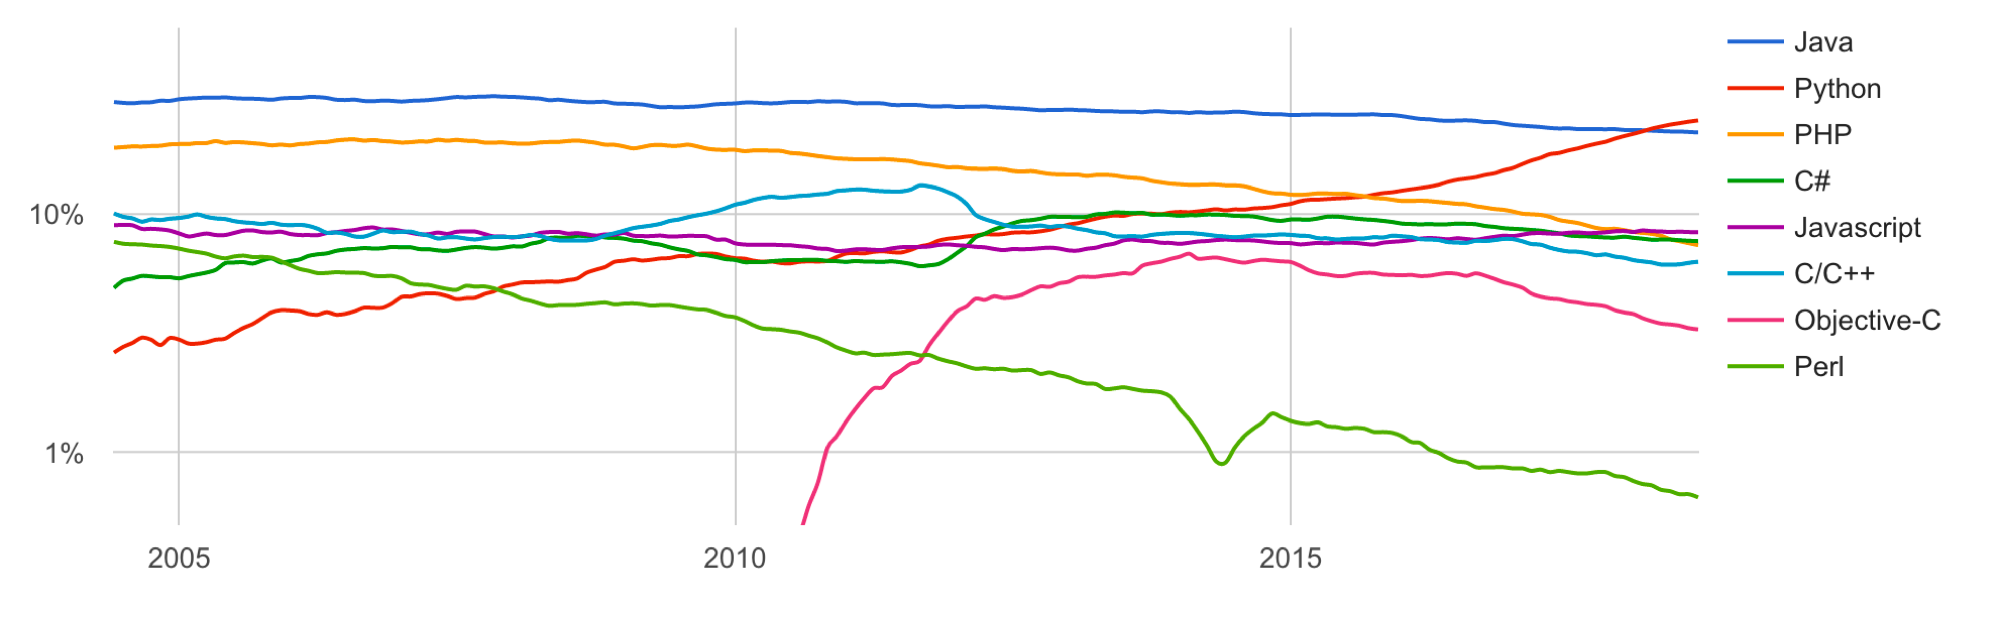
\includegraphics[width=\linewidth]{imgs/programminglanguangespopularity.png}
    \caption{PYPL popularity of programming languages~\cite{noauthor_pypl_2018}.}
    \label{fig:pypl}
\end{figure}

In particular, \citeauthor{noureddine_preliminary_2012}~\cite{noureddine_preliminary_2012} in 2012, and then Pereira~\emph{et~al.}~\cite{pereira_energy_2017} in 2017, conducted empirical power measurements on this topic: both concluded that compiled programming languages overcome dynamic ones when it comes to power consumption.
According to their experiments, an interpreted programming language, like Python, can impose up to a $7,588\,\%$ energy overhead compared to C~\cite{pereira_energy_2017} (cf. \Cref{fig:hannoi}).

\begin{figure}[!htb]
    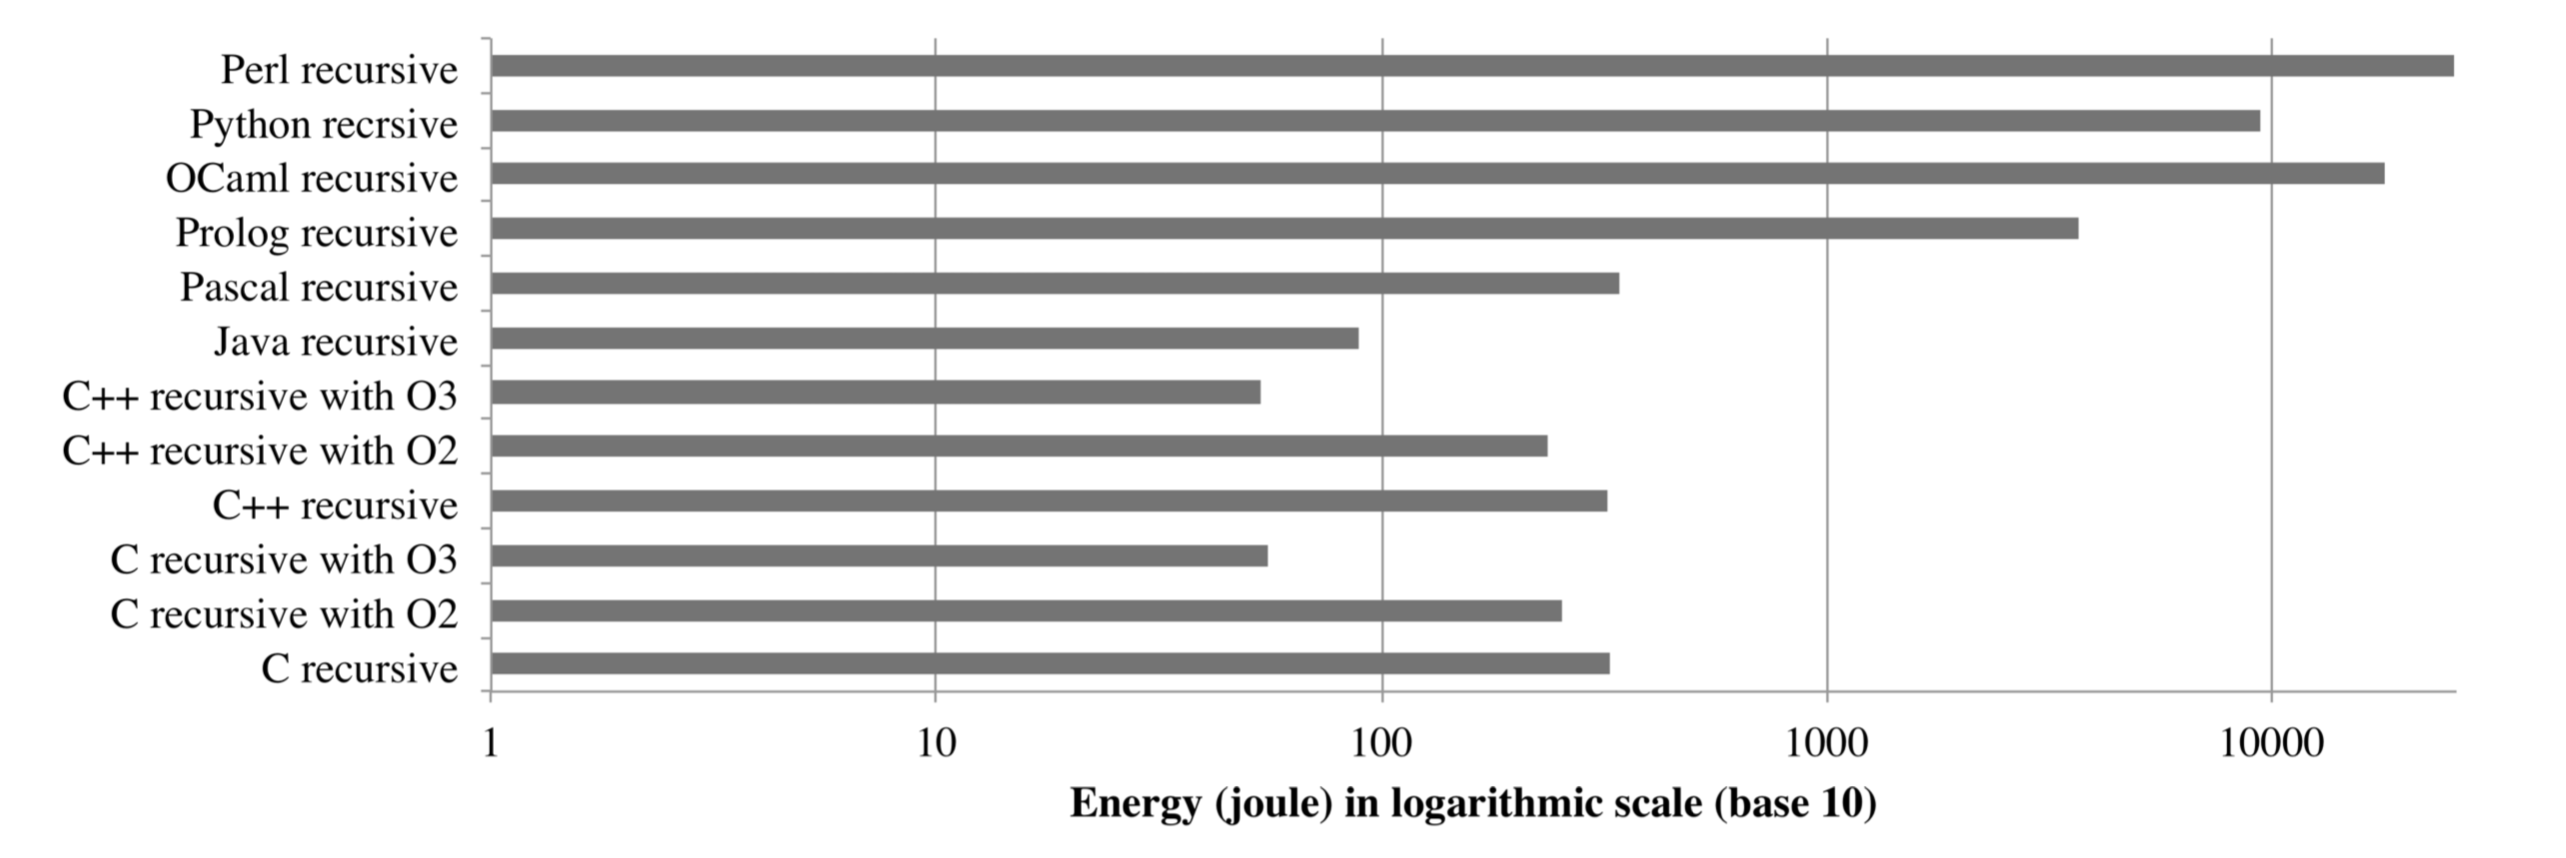
\includegraphics[width=\linewidth]{imgs/hannoiimplementation.png}
    \caption{Energy consumption of a recursive implementation of Tower of Hanoi program in different languages~\cite{noureddine_preliminary_2012}.}
    \label{fig:hannoi}
\end{figure}

In this chapter, we aim to reduce the energy consumption of Python code.
We first start by presenting the motivation behind our work in Section~\ref{python:sec_motivation}.
Then, we share some insights on the impact of programmer choices.
To do this, we report on a series of experiments to examine the energy consumption of Python code across various use cases.
Section~\ref{python:sec_insights} will then end by investigating several features of Python structure and their impact on energy consumption.
After that, in Section~\ref{python:sec_interpreters}, we investigate other non-intrusive approaches to optimizing the energy consumption of applications by comparing multiple Python runtime implementations, which include alternative interpreters and libraries that are dedicated to optimizing the code without changing its structures, such as \emph{ahead-of-time} (AOT) compilation and \emph{just-in-time} (JIT) libraries that are maintained by the community.


\section{Motivation}\label{python:sec_motivation}

\subsection{Python Popularity}
Nowadays, Python attracts a large community of developers who are interested in data analysis, web development, system administration, and machine learning.
According to a survey conducted in 2018 by JetBrains,\footnote{\url{https://www.jetbrains.com/research/python-developers-survey-2018/}} one can fear that the wide adoption of dynamic programming languages in production, like Python, may critically hamper the power consumption of ICT.
As the popularity of such dynamic programming languages partly builds on the wealth and the diversity of their ecosystem (\emph{e.g.}, the NumPY, SciKit\, Learn, and Panda libraries in Python), one cannot reasonably expect that developers will likely move to an alternative programming language mainly for energy considerations.
Rather, we believe that a better option consists of leveraging the strength of this rich ecosystem to promote energy-efficient solutions to improve the power consumption of legacy software systems.

\subsection{Python Gluttony}
% On the other hand, because of the interpreted nature of Python code, this programming language has paid a high price in terms of performance~\ref{fig:clbg}, memory and energy consumption.
According to~\cite{pinto_energy_2017} and~\cite{noureddine_preliminary_2012}, Python tends to be one more energy hungry programming language.
As one can notice in \Cref{fig:hannoi}, Python consumes $30$ times more than C or C++.
The benchmark was implemented with the \fnurl{Tower of Hanoi}{https://en.wikipedia.org/wiki/Tower_of_Hanoi} of 30 disks.

As shown in \Cref{fig:clbg}, one can observe that, for most of the applications taken for the \emph{Computer Language Benchmark Game} (CLBG), Python takes more time to execute---the only case that he was not the worst one was in the benchmark \textsf{regx-redux} where he beats Go---and in some cases the gap was huge, such as in \textsf{n-body} where Python took around $100$ times more than C++.\footnote{\url{https://benchmarksgame-team.pages.debian.net/benchmarksgame/index.html}}

\begin{table}[hbt]
    \centering
    \caption{Comparison of CLBG execution times (in seconds) depending on programming languages.}
    \label{fig:clbg}
    \begin{tabular}{l|*{5}r}
        \hline
                                    & \bf C       & \bf C++     & \bf Java & \bf Python     & \bf Go        \\
        \hline
        \hline
        \textsf{pidigits}           & \best{1.75} & 1.89        & 3.13     & \worst{3.51}   & 2.04          \\
        \textsf{reverse-complement} & \best{1.75} & 2.95        & 3.31     & \worst{16.76}  & 4.00          \\
        \textsf{regx-redux}         & \best{1.45} & 1.66        & 10.5     & 15.56          & \worst{28.69} \\
        \textsf{k-nucleotide}       & 5.07        & \best{3.66} & 8.66     & \worst{79.79}  & 15.36         \\
        \textsf{binary-trees}       & \best{2.55} & 2.63        & 8.28     & \worst{92.72}  & 28.90         \\
        \textsf{fasta}              & \best{1.32} & 1.33        & 2.32     & \worst{62.88}  & 2.07          \\
        \textsf{Fannkuch-redux}     & \best{8.72} & 10.62       & 17.9     & \worst{547.23} & 17.82         \\
        \textsf{n-body}             & 9.17        & \best{8.24} & 22.0     & \worst{882.00} & 21.00         \\
        \textsf{spectral-norm}      & 1.99        & \best{1.98} & 4.27     & \worst{193.86} & 3.95          \\
        \textsf{Mandelbort}         & 1.64        & \best{1.51} & 6.96     & \worst{279.68} & 5.47          \\
        \hline
    \end{tabular}
\end{table}

Python consumes energy mainly because it is slow in execution.
Its flexibility and simplicity caused it to drop off in performance because Python gains its flexibility from being a dynamic language.
Therefore, it requires a faster interpreter to execute its programs to compete against alternatives written in compiled programming languages, such as C and C++, or semi-compiled languages, like Java.

\subsection{Python Use Cases}
To reduce the energy consumption of Python, we started by targeting the main usage of this programming language, which is revealed to be data science and web development.
\Cref{fig:usecase} illustrates a study published by the JetBrain company on Python developers.\footnote{\url{https://www.jetbrains.com/lp/python-developers-survey-2020}}
57\% of the respondents reported that they use Python for data science, and 51\% said they use it for web development.
Around 40\% are using it for system administration.\footnote{The options in this survey were not mutually exclusive. As a result, the total of the percentages is greater than $100\%$.}

\begin{figure}[hbt]
    \centering
    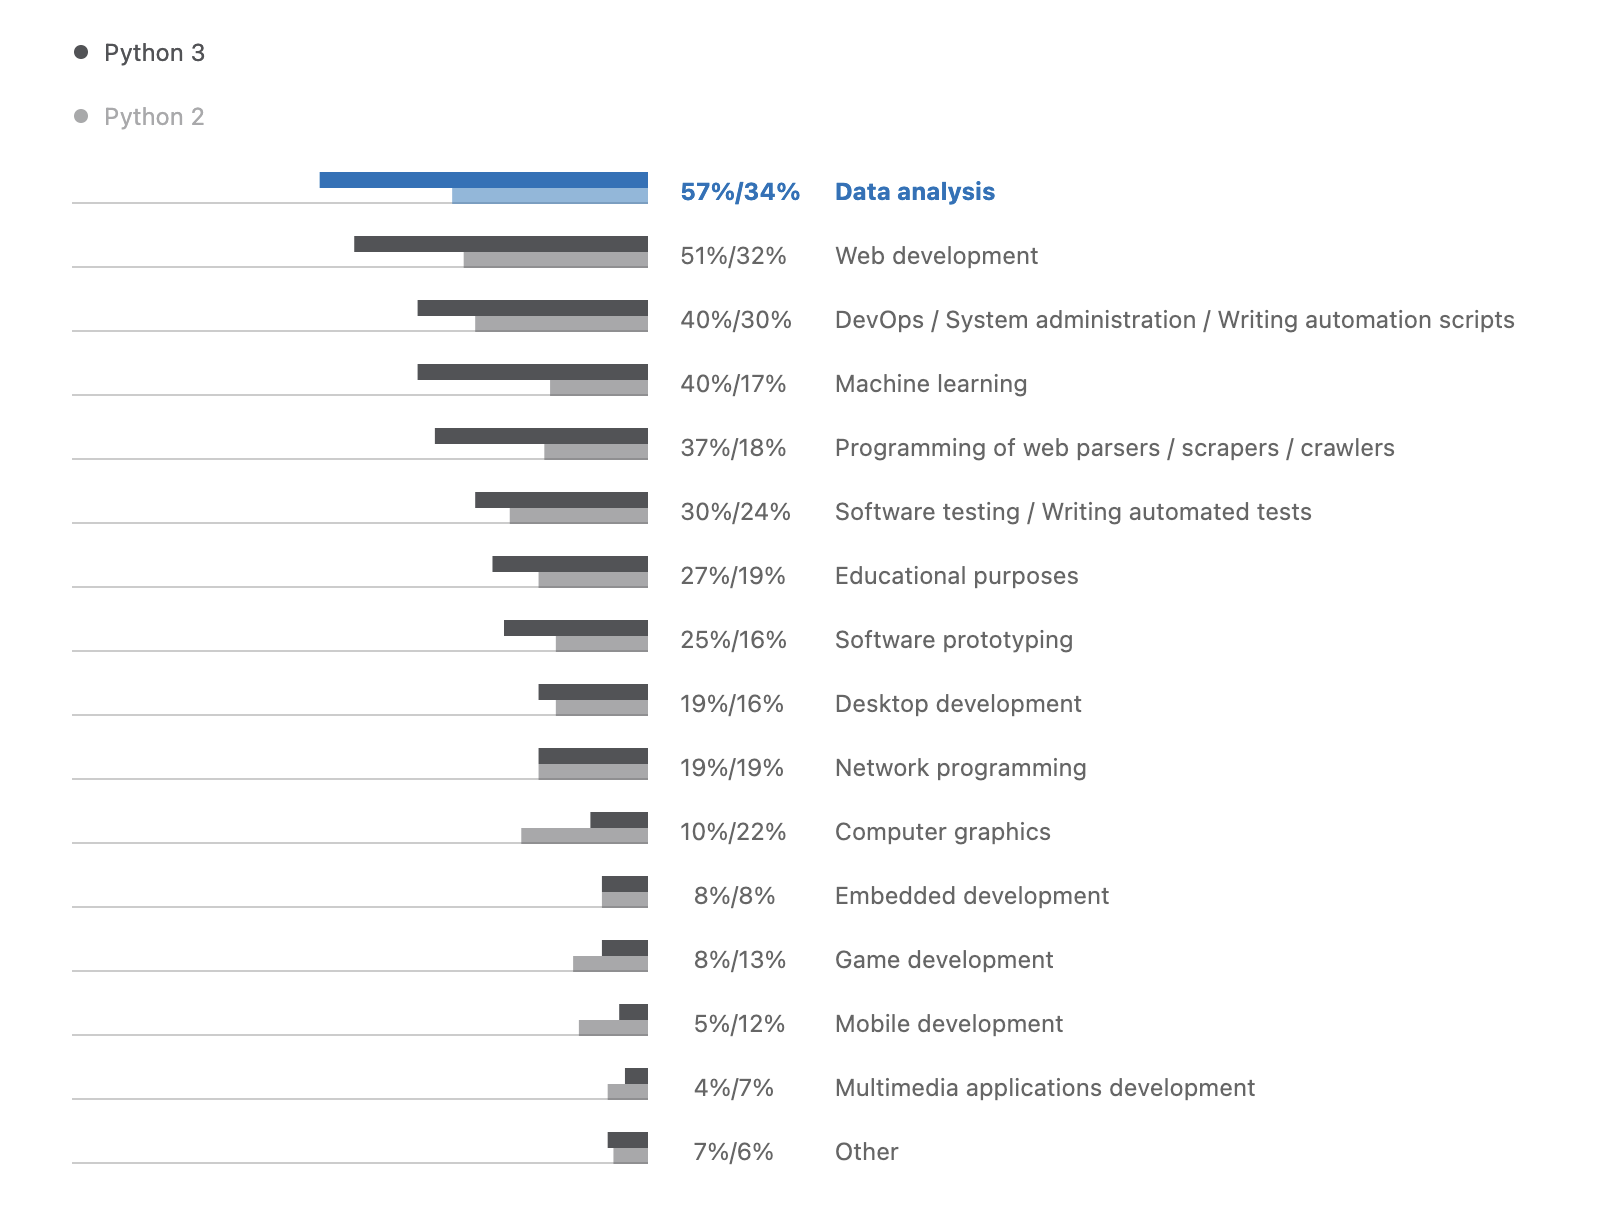
\includegraphics[width=\linewidth]{imgs/python_use_cases}
    \caption{Use cases of Python (source: JetBrain).}
    \label{fig:usecase}
\end{figure}

\section{Optimizing the Energy Consumption of Python Applications}\label{python:sec_insights}
In this section, we study the energy footprint of Python in its most popular domains of adoption.
We first explore the data and control structures, aiming to reveal some fundamental guidelines, as \citeauthor{hasan_energy_2016} did in~\cite{hasan_energy_2016}.
Then, we measure the energy consumption of several Python implementations to propose a non-intrusive technique to improve energy efficiency.
Overall, this section will address the following research questions:
\begin{compactenum}[\indent\bf RQ\,1:]
    \item \emph{What is the energy footprint of Python when used in data science?}
    \item \emph{Are the Python guidelines energy-efficient by construction?}
    \item \emph{Can we reduce the energy consumption of Python programs without altering the source code?}
\end{compactenum}

To answer these questions, we report on 4 case studies that intend to answer these research questions.
First, we study the energy behavior of Python in two application contexts: machine learning (cf. \Cref{sec:webdev}) and web applications (cf. \Cref{sec:ml}).
Then, we dive deeper into the energy consumption of Python core structures before concluding with the impact of parallelism on energy consumption.

\subsection{Python for Machine Learning}\label{sec:ml}
Machine learning is becoming an integral part of our daily lives, growing more potent and energy-hungry each year.
As machine learning can significantly impact climate change, it is vital to investigate mitigation techniques.

\subsubsection{Experimental Protocol}
\paragraph{Measurement Context}
\subparagraph{Hardware settings:}
Chifflot\,8 from Grid 5000's Lille site was used for all of the trials.
The machine is outfitted with two Intel Xeon Gold 6126 CPUs, each having 12 physical cores, 192 GB of RAM, and two 32 GB Tesla V100 GPUs.

\subparagraph{Software settings:}
Each experiment is done within a Docker container using Jupyter lab to ensure reproducibility.
These tests are run atop a minimal version of Debian-10 to increase the tests' accuracy by eliminating unnecessary processes.

\subsubsection{Input Workload}
\subparagraph{Models:}
Several models were developed.
However, only two were used in the final trials because they achieved 94\% accuracy with an acceptable training time.
David Page's \textsf{cifar10-fast}\footnote{\url{https://github.com/davidcpage/cifar10-fast}} and Woonhyuk Baek's torch skeleton\footnote{\url{https://github.com/wbaek/torchskeleton}} are reported here.

\subparagraph{Datasets:}
The CIFAR-10 dataset was the major source of data for the studies.
It is made up of $60,000$ \texttt{32x32} color images grouped into $10$ categories.

Some experiments were done using the MNIST dataset of handwritten digits to validate the results acquired from the first dataset.
The model did not need to be updated because the $60,000$ \texttt{28x28} grayscale photos were padded.

\paragraph{Candidates:}
The experiments were run with several different CPU and GPU configurations:
\begin{itemize}
    \item with and without GPU,
    \item with and without CPU hyper-threading,
    \item different number of CPU physical cores.
\end{itemize}

\paragraph{Key Performance Metrics:}
We used Pytorch 1.10.0 to train those models and pyJoules to measure the energy consumption of the GPU and CPU.
The key performance metrics are, therefore:
\begin{itemize}
    \item \emph{accuracy}: in \%
    \item \emph{execution time}: in seconds for both the duration of each epoch and the total duration to achieve a certain accuracy
    \item \emph{total energy consumption}: in joules, including the CPU and the GPU.
\end{itemize}


\subsubsection{Results \& Findings}
As the model's accuracy increases, so do the energy required for the next accuracy increment.
Figure~\ref{fig:cum_energy_vs_accuracy} depicts how the curve steepens as training progresses.
For example, training to 90\% accuracy requires three times the energy required for training to 80\% accuracy.

\Cref{fig:eopochvsaccuracy} shows the model's accuracy based on the number of epochs.
This figure shows that there is a non-significant impact on the choice of the strategy on the accuracy; it is only a matter of the number of epochs.
However, the increase in accuracy is not linear, as can be observed.
It took only 10 epochs to reach an accuracy of 84\%, but it required more than twice the number of epochs to add an extra 6\% accuracy.
This highlights the price one should pay to increase the model's accuracy.

\begin{figure}
    \centering
    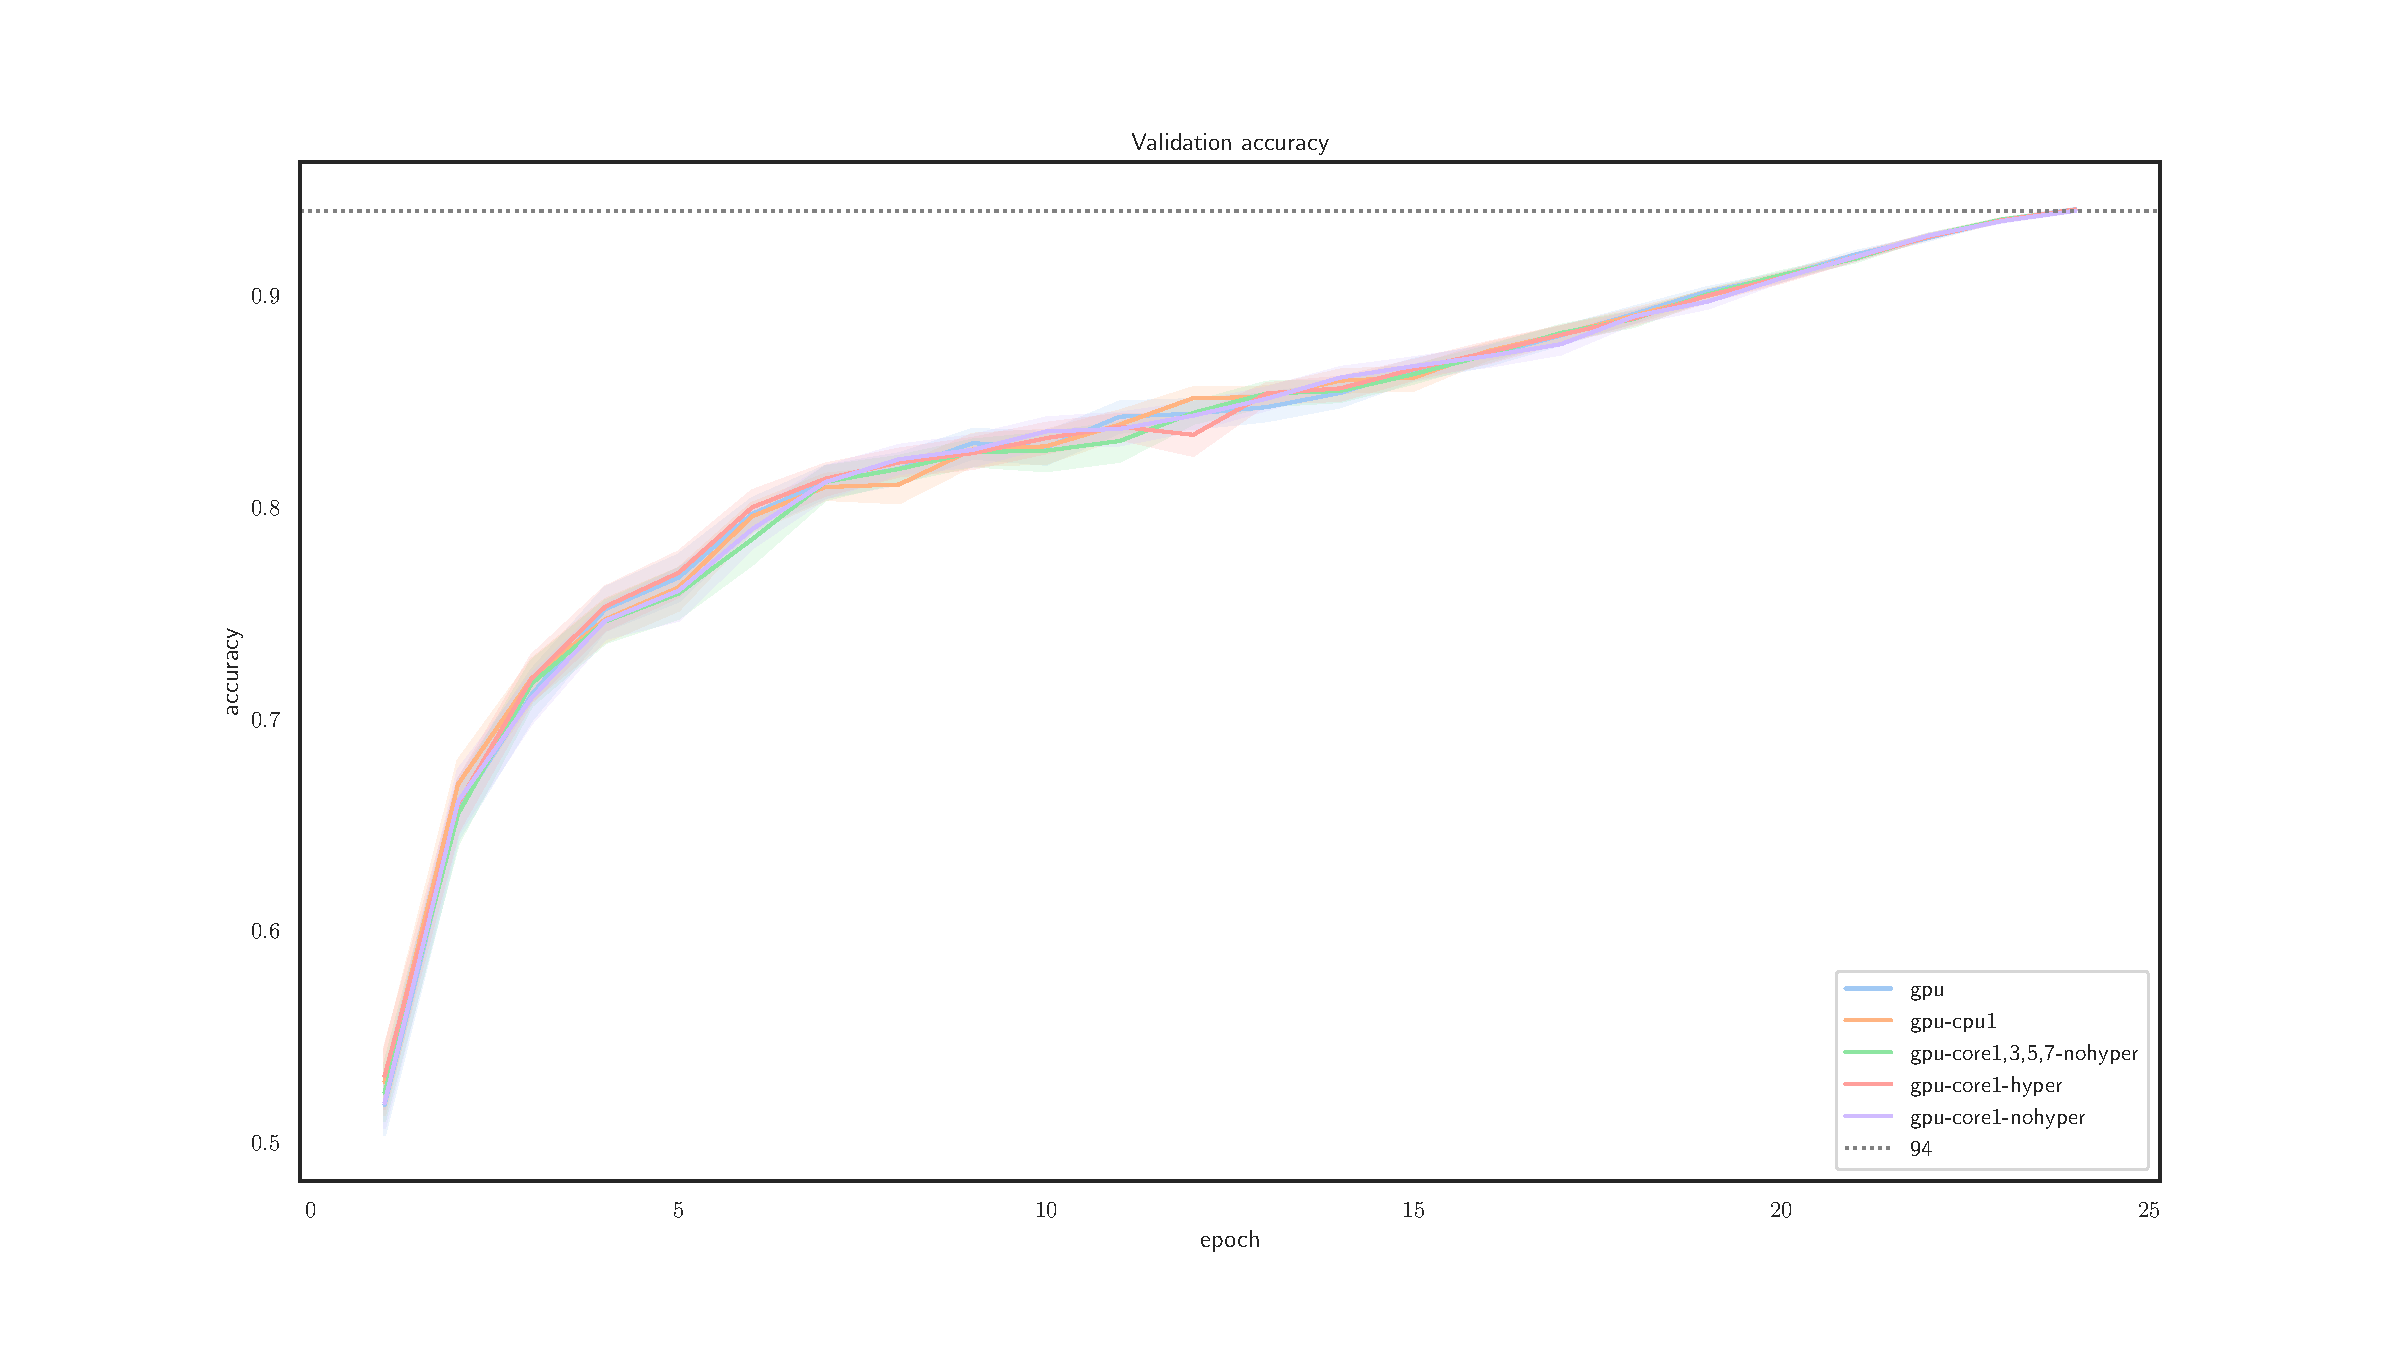
\includegraphics[width=1.1\textwidth]{imgs/accuracy_basedonepoch}
    \caption{Accuracy along epochs.}
    \label{fig:eopochvsaccuracy}
\end{figure}

\Cref{fig:cum_energy_vs_accuracy} confirm this observation.
As one can see, the training of the model up to 90\% accuracy requires three times the energy required for training to 80\% accuracy.
Moreover, one can notice that this price is paid mainly by the CPU and GPU, while the memory is not that impacted.

\begin{figure}
    \centering
    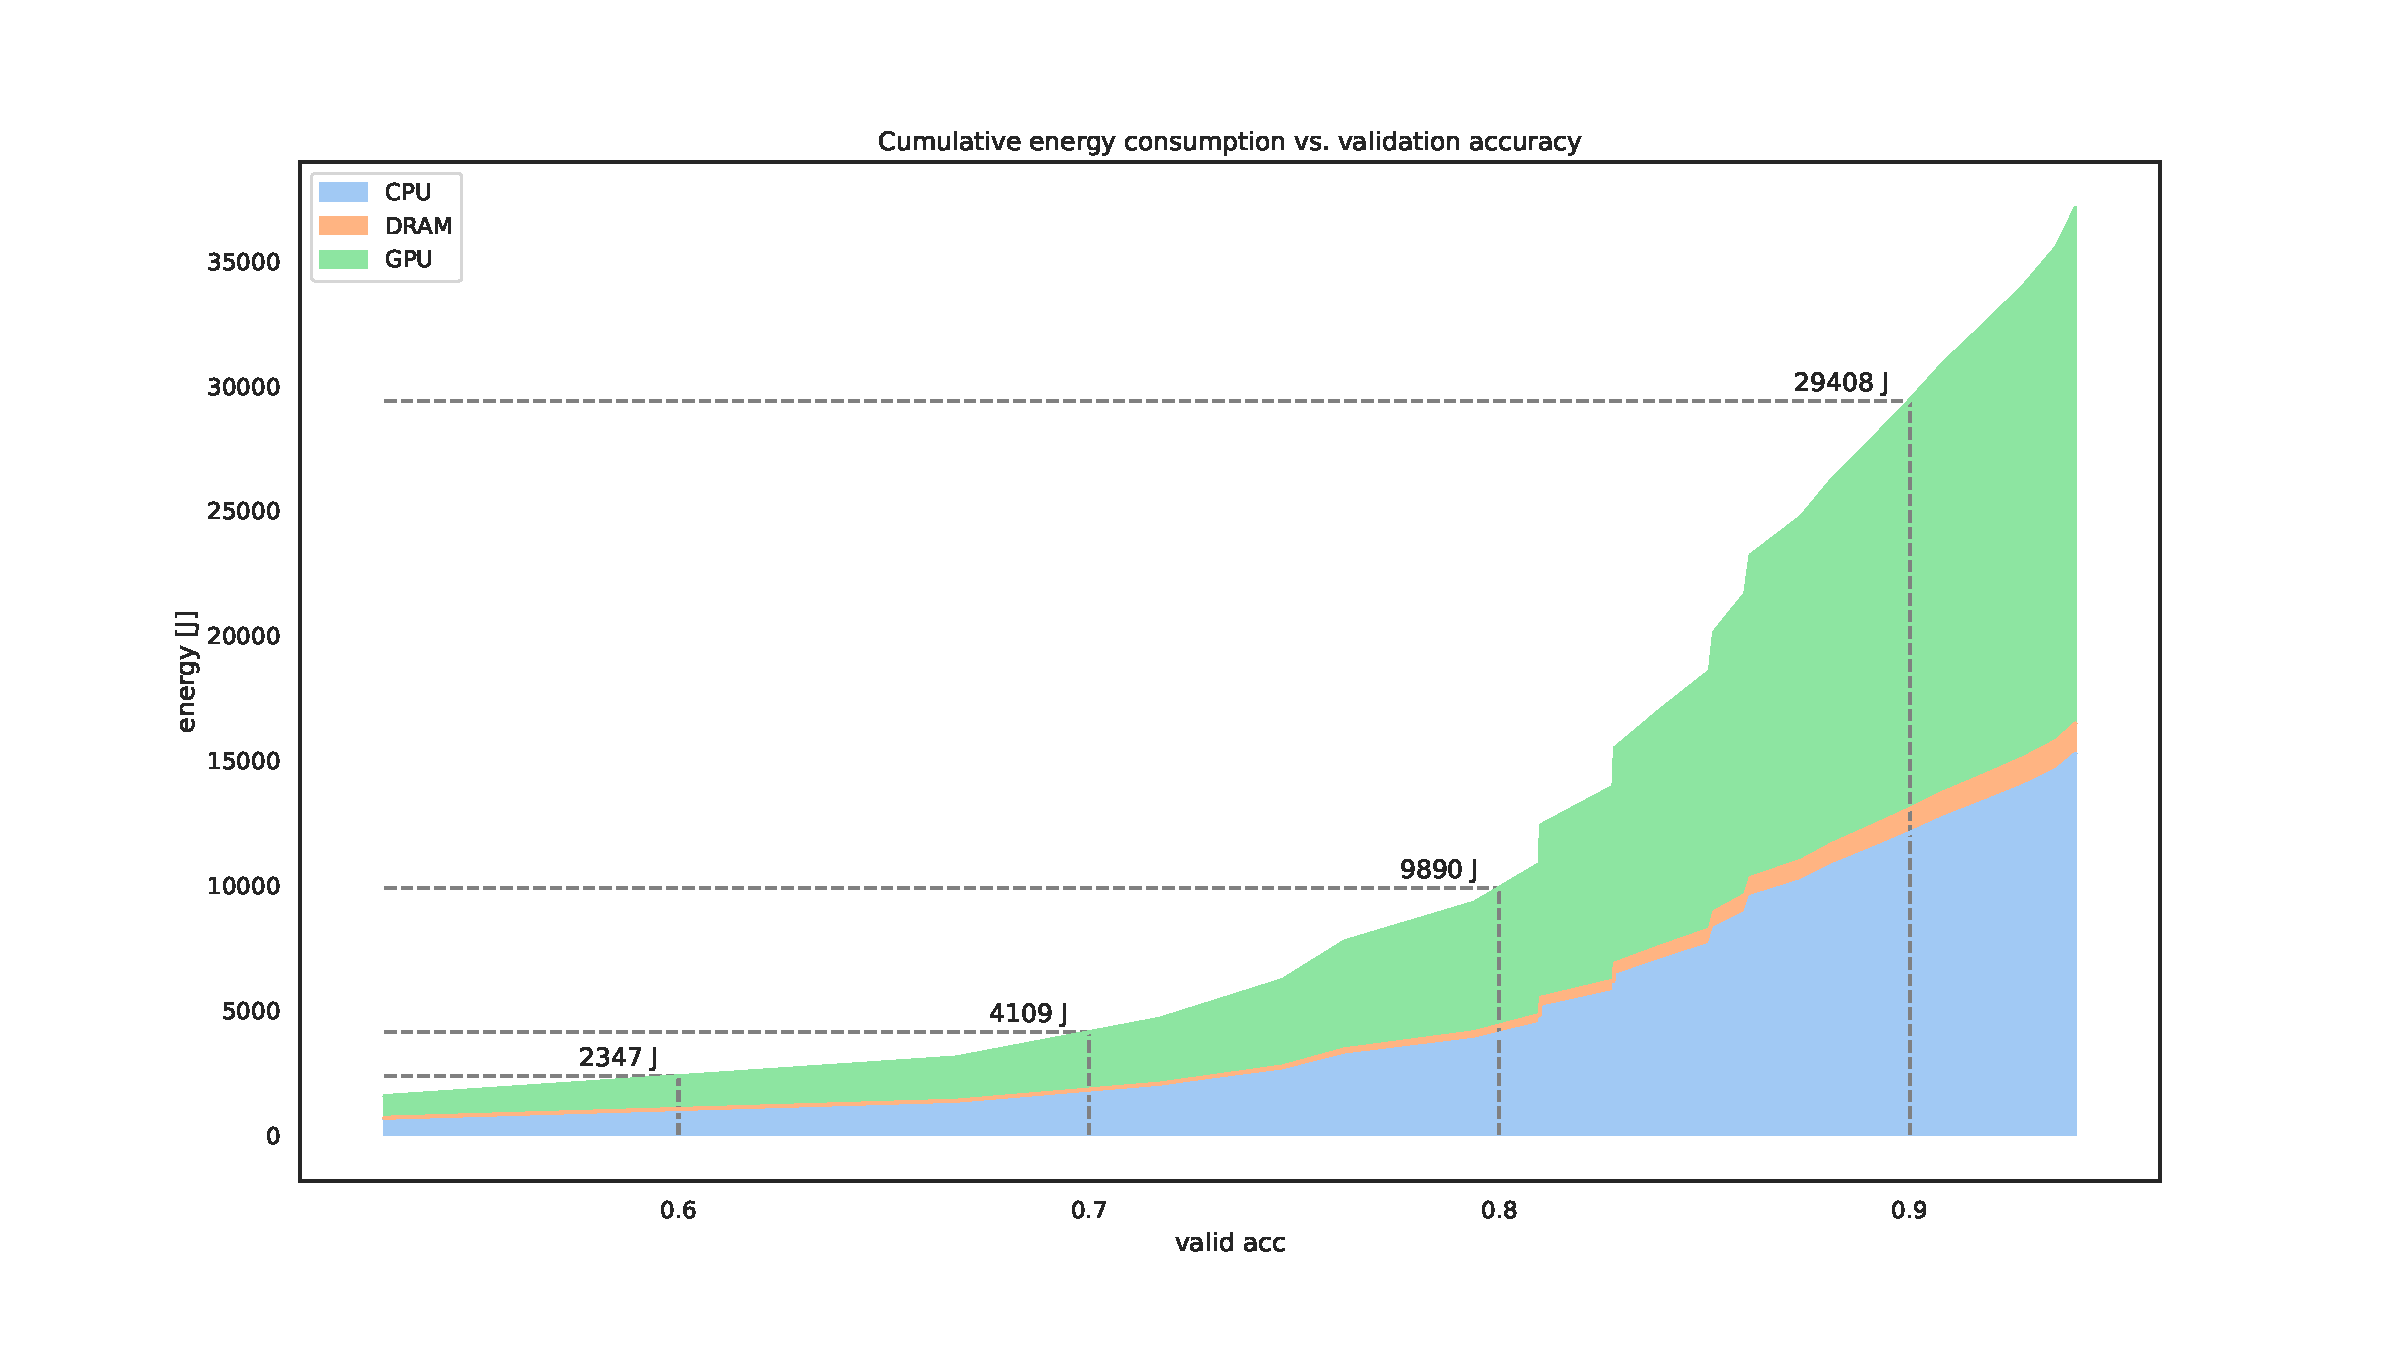
\includegraphics[width=1.1\textwidth]{imgs/cumulative_energy_vs_accuracy}
    \caption{Cumulative energy consumption vs. accuracy.}
    \label{fig:cum_energy_vs_accuracy}
\end{figure}

Interestingly there were no significant differences between different strategies---around $1.3\%$---as shown in Figure~\ref{fig:av_energy_setup}.
However, this gap may increase as the number of epochs increases.

\begin{figure}
    \centering
    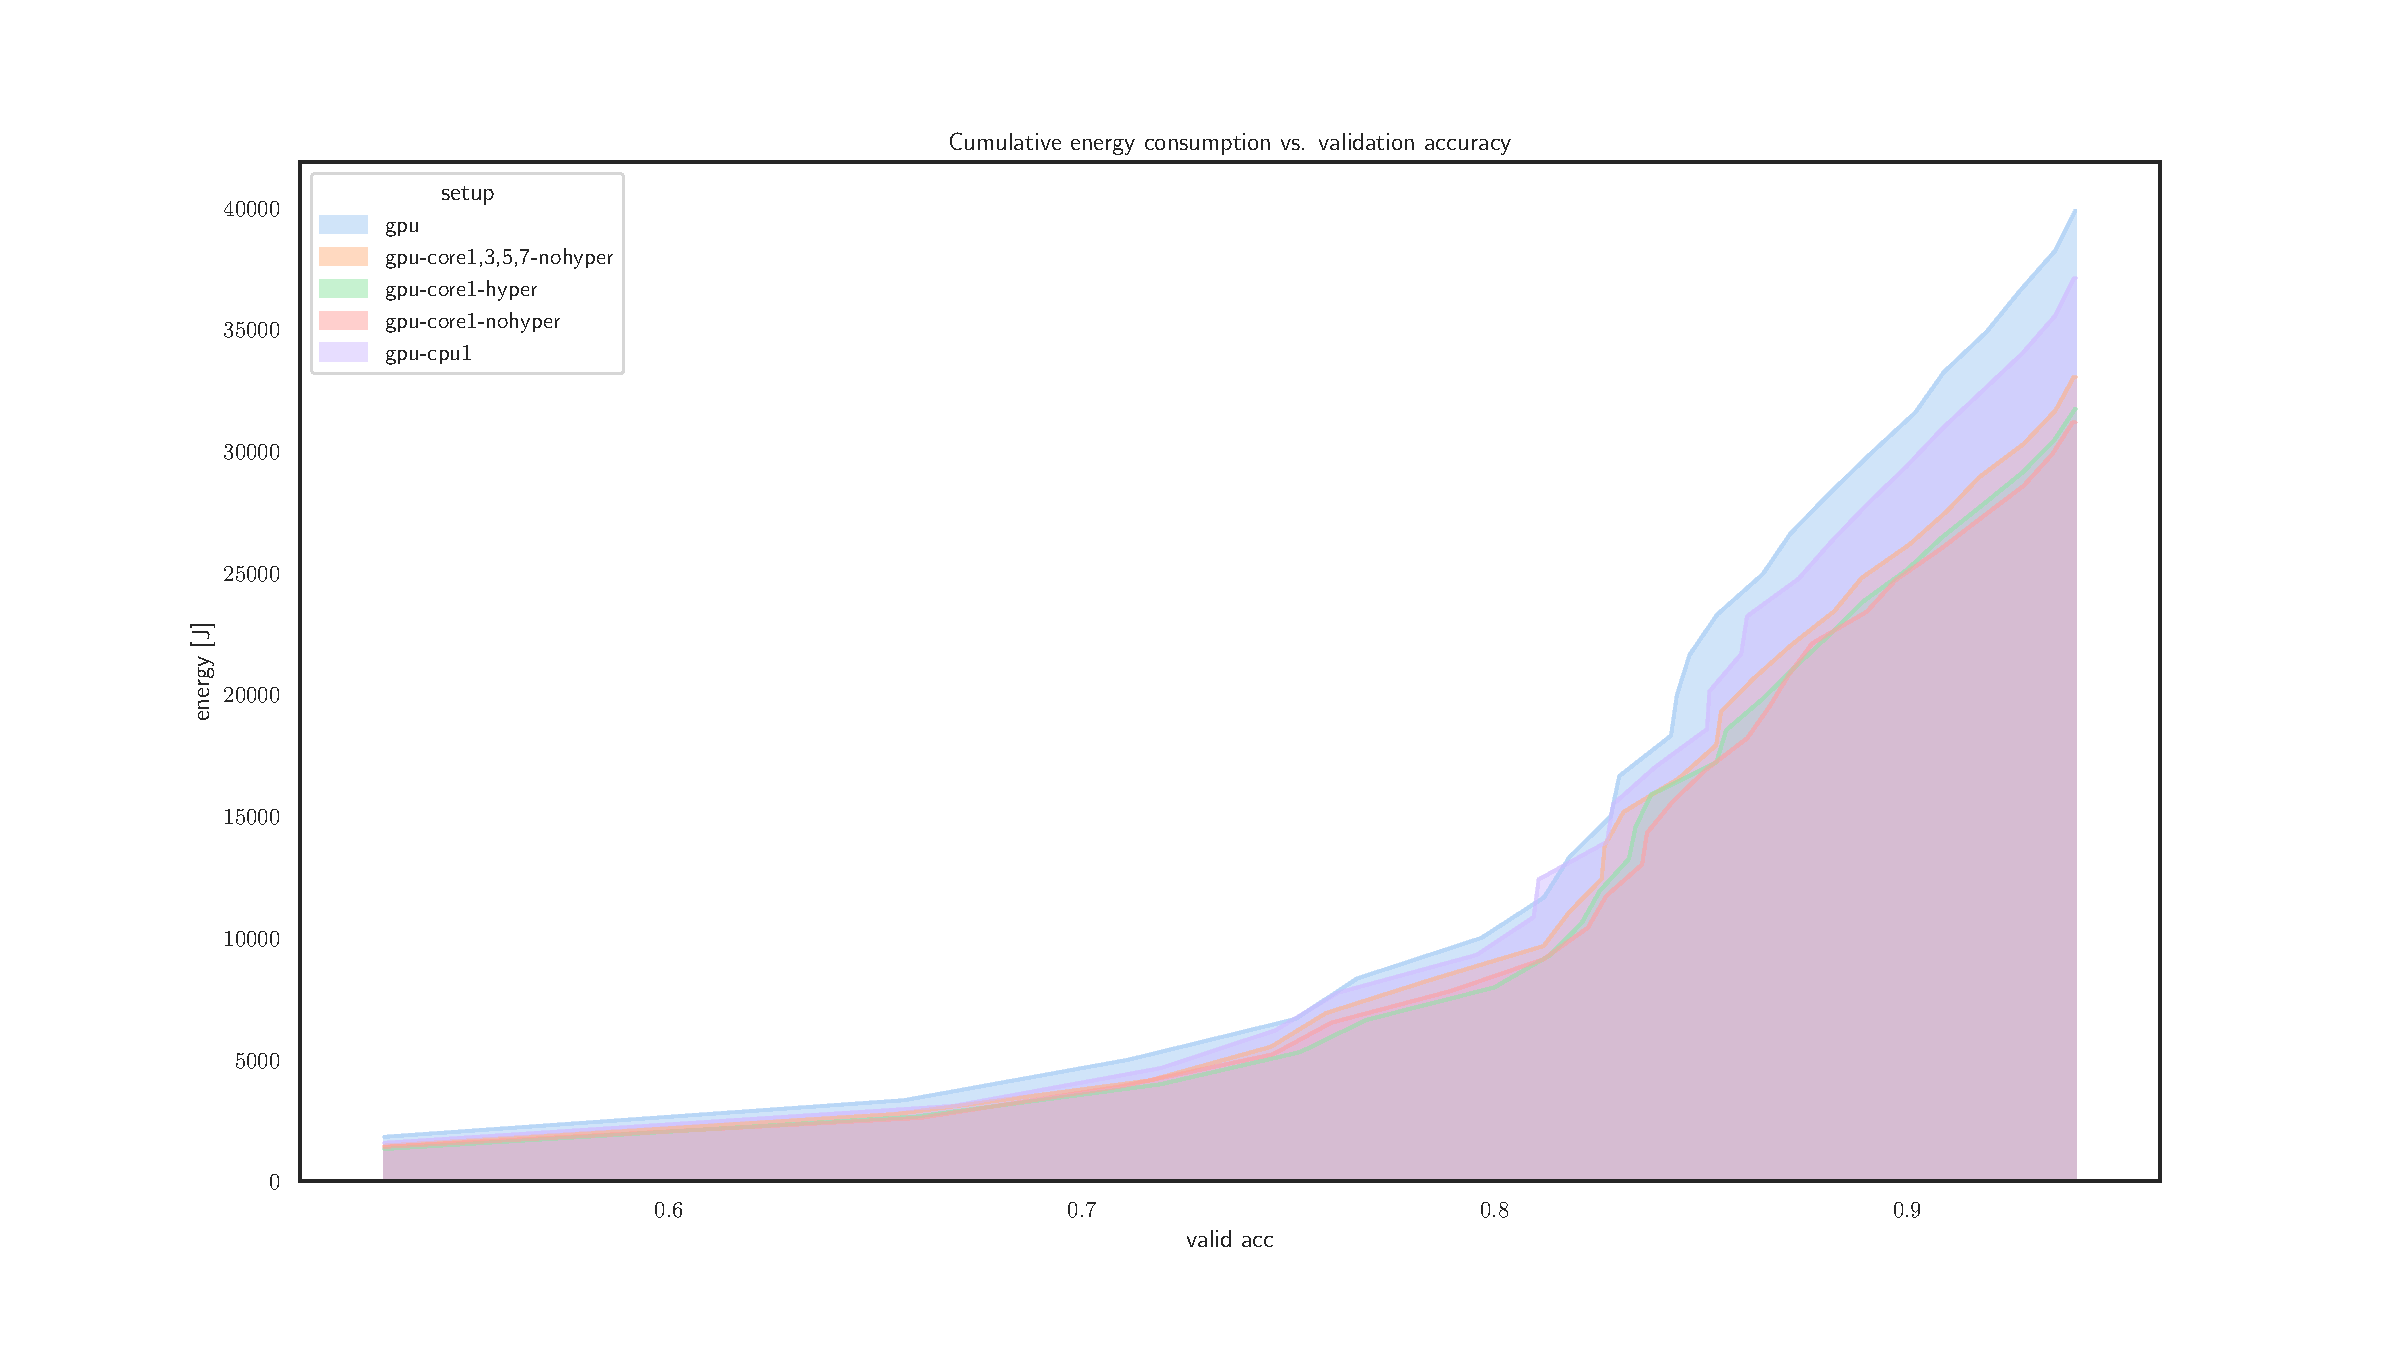
\includegraphics[width=1.1\textwidth]{imgs/cumulative_energy_fast10.pdf}
    \caption{Average energy for training the model based on the strategy.}
    \label{fig:av_energy_setup}
\end{figure}

On the other hand, as the number of epochs increases, the average power consumption decreases until it reaches a steady state after 10 epochs.
This could be connected to the caching strategies adopted by the CPU and GPU.
However, this evolution is still insignificant compared to the baseline value.
This is shown in Figure~\ref{fig:ephoch_power}.

\begin{figure}
    \centering
    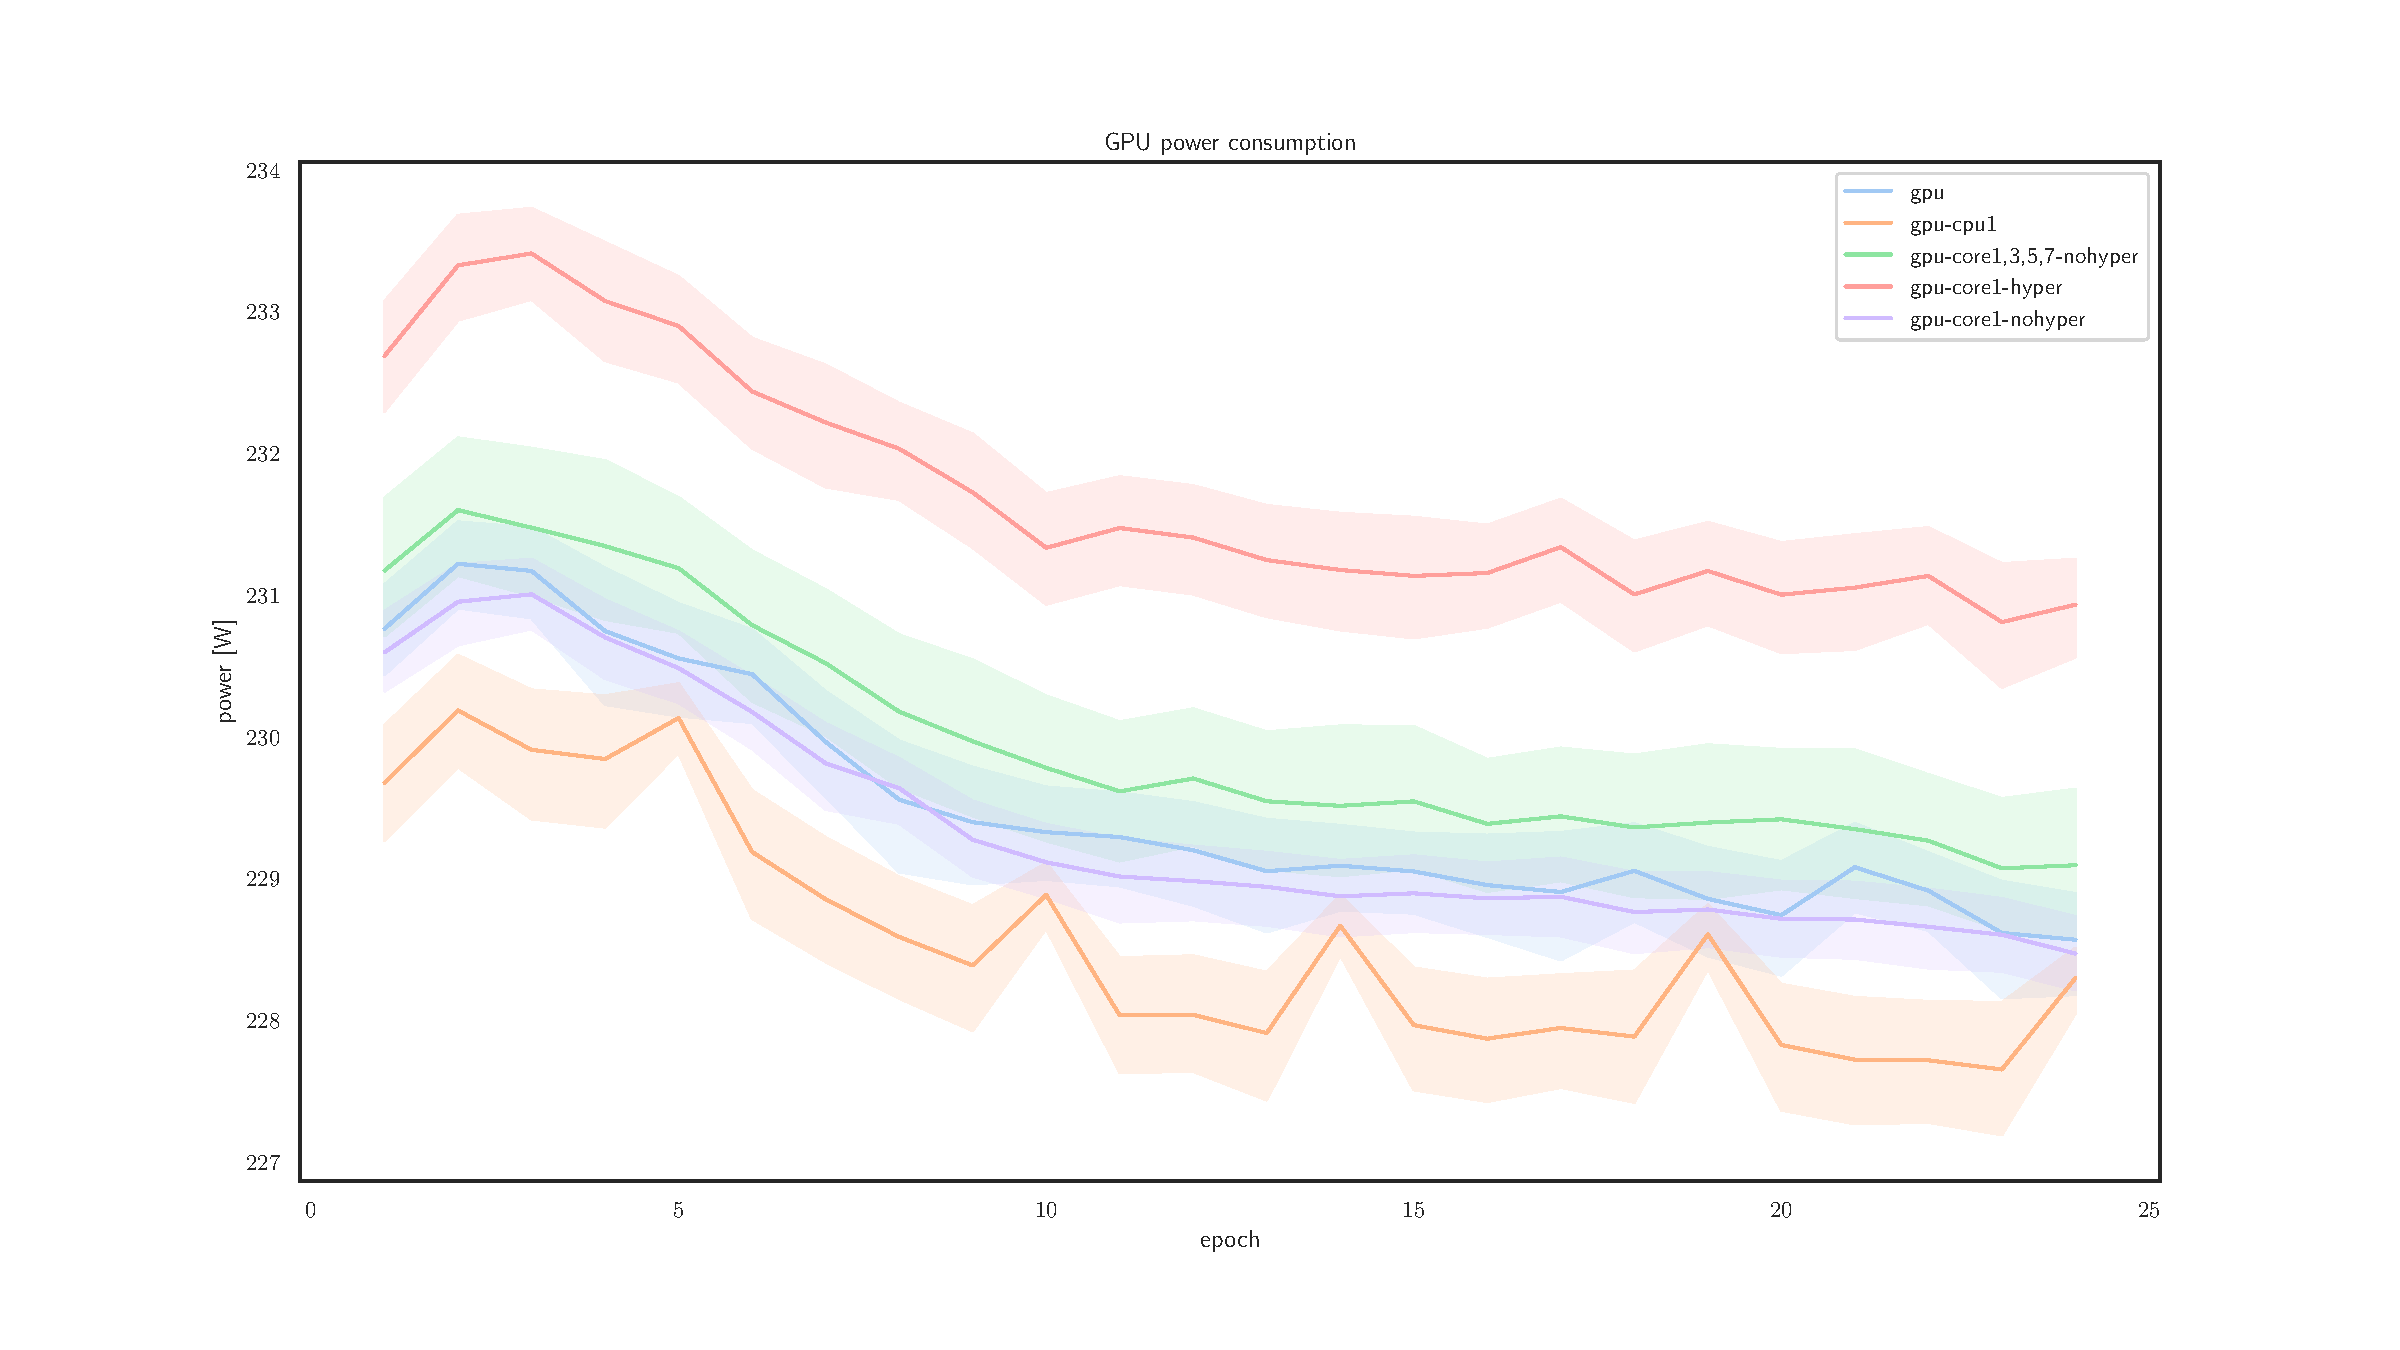
\includegraphics[width=1.1\textwidth]{imgs/power_gpu_baedonepoche.pdf}
    \caption{Evolution of average GPU power along epochs.}
    \label{fig:ephoch_power}
\end{figure}

As one can see in Figures~\ref{fig:ephoch_power} and~\ref{fig:epoch_duration}, the average power consumption and the average duration of an epoch do not have a significant variation, as most of them last around 3.7 seconds.
However, these two values have an intermediate correlation if we exclude the strategy based on one core and its hyper-thread.
The last strategy exhibits more power- even when its duration is not optimal- because the context switches between the core and its hyper-thread.

\begin{figure}
    \centering
    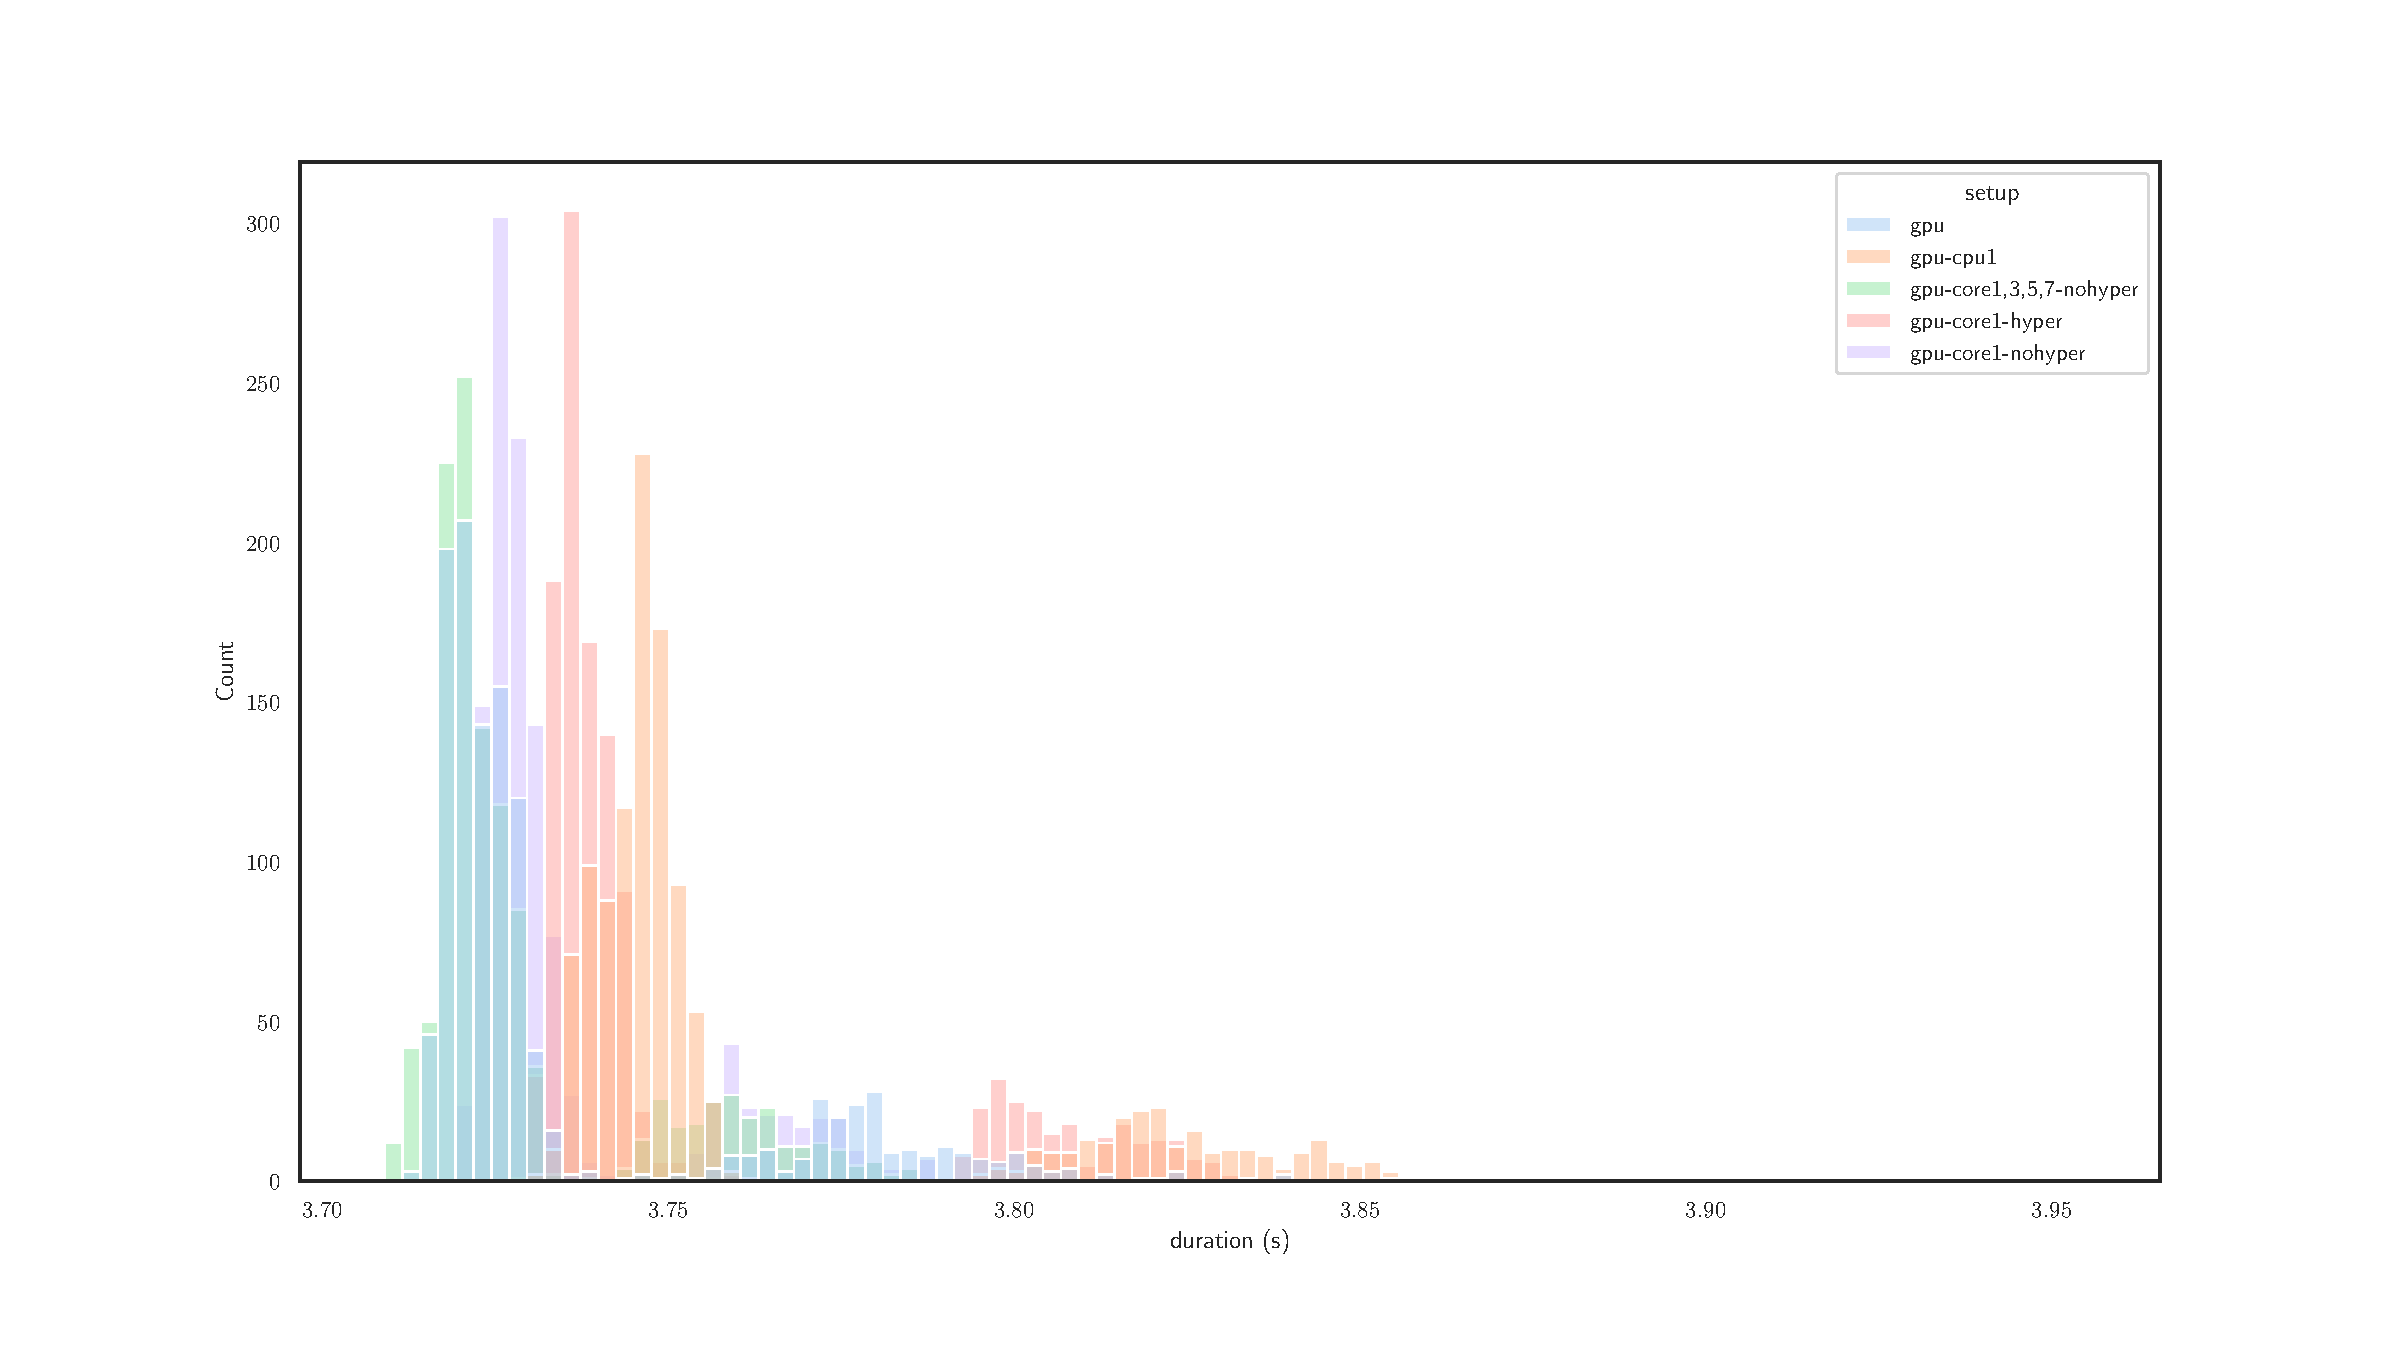
\includegraphics[width=1.1\textwidth]{imgs/epoch_duration.pdf}
    \caption{Distribution of the durations of each epoch.}
    \label{fig:epoch_duration}
\end{figure}

\subsubsection{Synthesis}
We discovered that when the model's accuracy improves, so does the energy required for a subsequent accuracy gain.
This begs the question of when we should discontinue training.
Is a 10\% increase in accuracy worth it if we have to spend three times the energy?
While using the GPU, the CPU has no significant impact on the energy consumption of the training.
Therefore, one can limit the number of CPU cores used during the execution without sacrificing the execution time and accuracy.


\subsection{Python for Web Development}\label{sec:webdev}
Django\footnote{\url{https://www.djangoproject.com/}} and Flask\footnote{\url{https://flask.palletsprojects.com/}} are the most popular Pyhton frameworks for web development.
According to a Jetbrains poll,\footnote{\url{https://lp.jetbrains.com/python-developers-survey-2021/}} Django is used in 40\% of the cases, while Flask is used in 41\% of the cases.

In contrast to Flask, which is a micro-framework, Django is a high-level web framework that provides a standard method for creating and maintaining complex and scalable database-driven websites quickly and effectively.
Therefore, this study will focus on the latter one.

\paragraph{Life-cycle of a request in Django}
Django is an MVT (\emph{Model-View-Template}) framework, which means that it follows the MVC (\emph{Model-View-Controller}) pattern.
Figure~\ref{fig:django-life-cycle} describes the life-cycle of a request in this framework.
Whenever a request arrives in Django, it is processed by the middleware layers, one at a time.
These middleware layers are in charge of authentication, security, and so on.
Once these layers process the request, it is passed to the URL router, which extracts the URL from the request and tries to match it to the defined URLs.
After getting the matching URL, the corresponding view function is called.
This function is responsible for treating the request, gathering the data, and then generating the response that will be put inside a template to be returned as a response.
As Django adopts an MVT model, it also offers an automatic way to retrieve data from the database to the view using the \emph{Object Relational Mapping} (ORM)~\cite{o2008object}.

\begin{figure}[!htb]
    \centering
    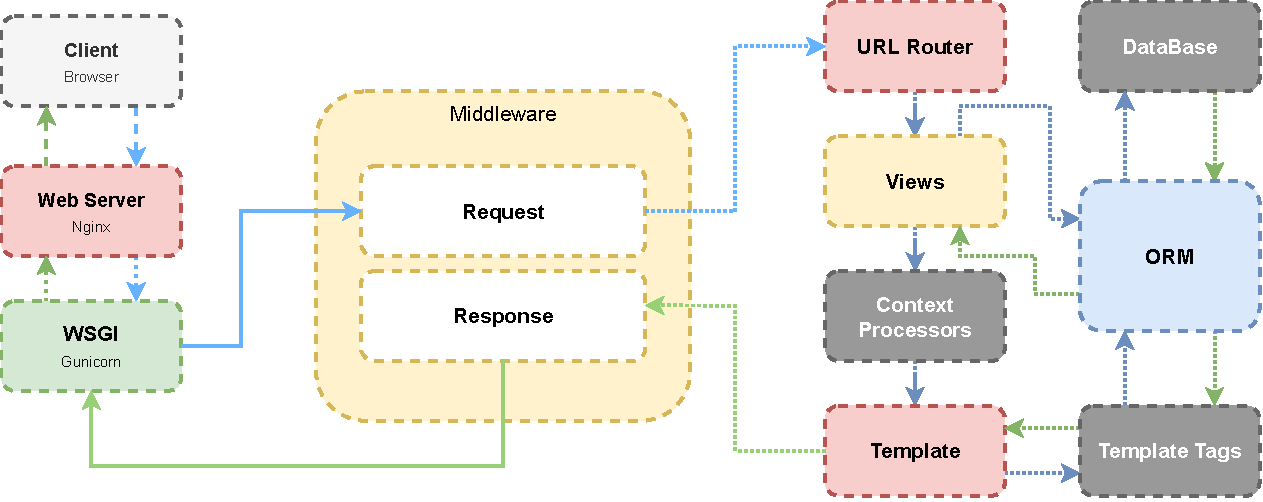
\includegraphics[width=.9\linewidth]{imgs/django_request_lifecycle}
    \caption{Request-Response life cycle in Django}
    \label{fig:django-life-cycle}
\end{figure}

First, we investigate the energy consumption of the request-response life cycle in Django to determine which layer consumes the most energy.
To do so, we created a sample Django application that returns the response to the request.
We tracked its energy consumption using JouleHunter.\footnote{\url{https://github.com/powerapi-ng/joulehunter}}
JouleHunter is an open-source library that we developed to help practitioners identify energy hotspots in their applications using statistical profilers.
In the case of Django, JouleHunter is included as a middleware with no additional setup or change to the source code.
The energy consumption of the request-response life-cycle in Django is shown in Figure~\ref{fig:django_life_cycle_naive}.
As we can notice, 91.4\% of the total energy consumption is spent on resolving the request by retrieving the data, while only 5.27\% is consumed on rendering the response.

\begin{figure}[!htb]
    \centering
    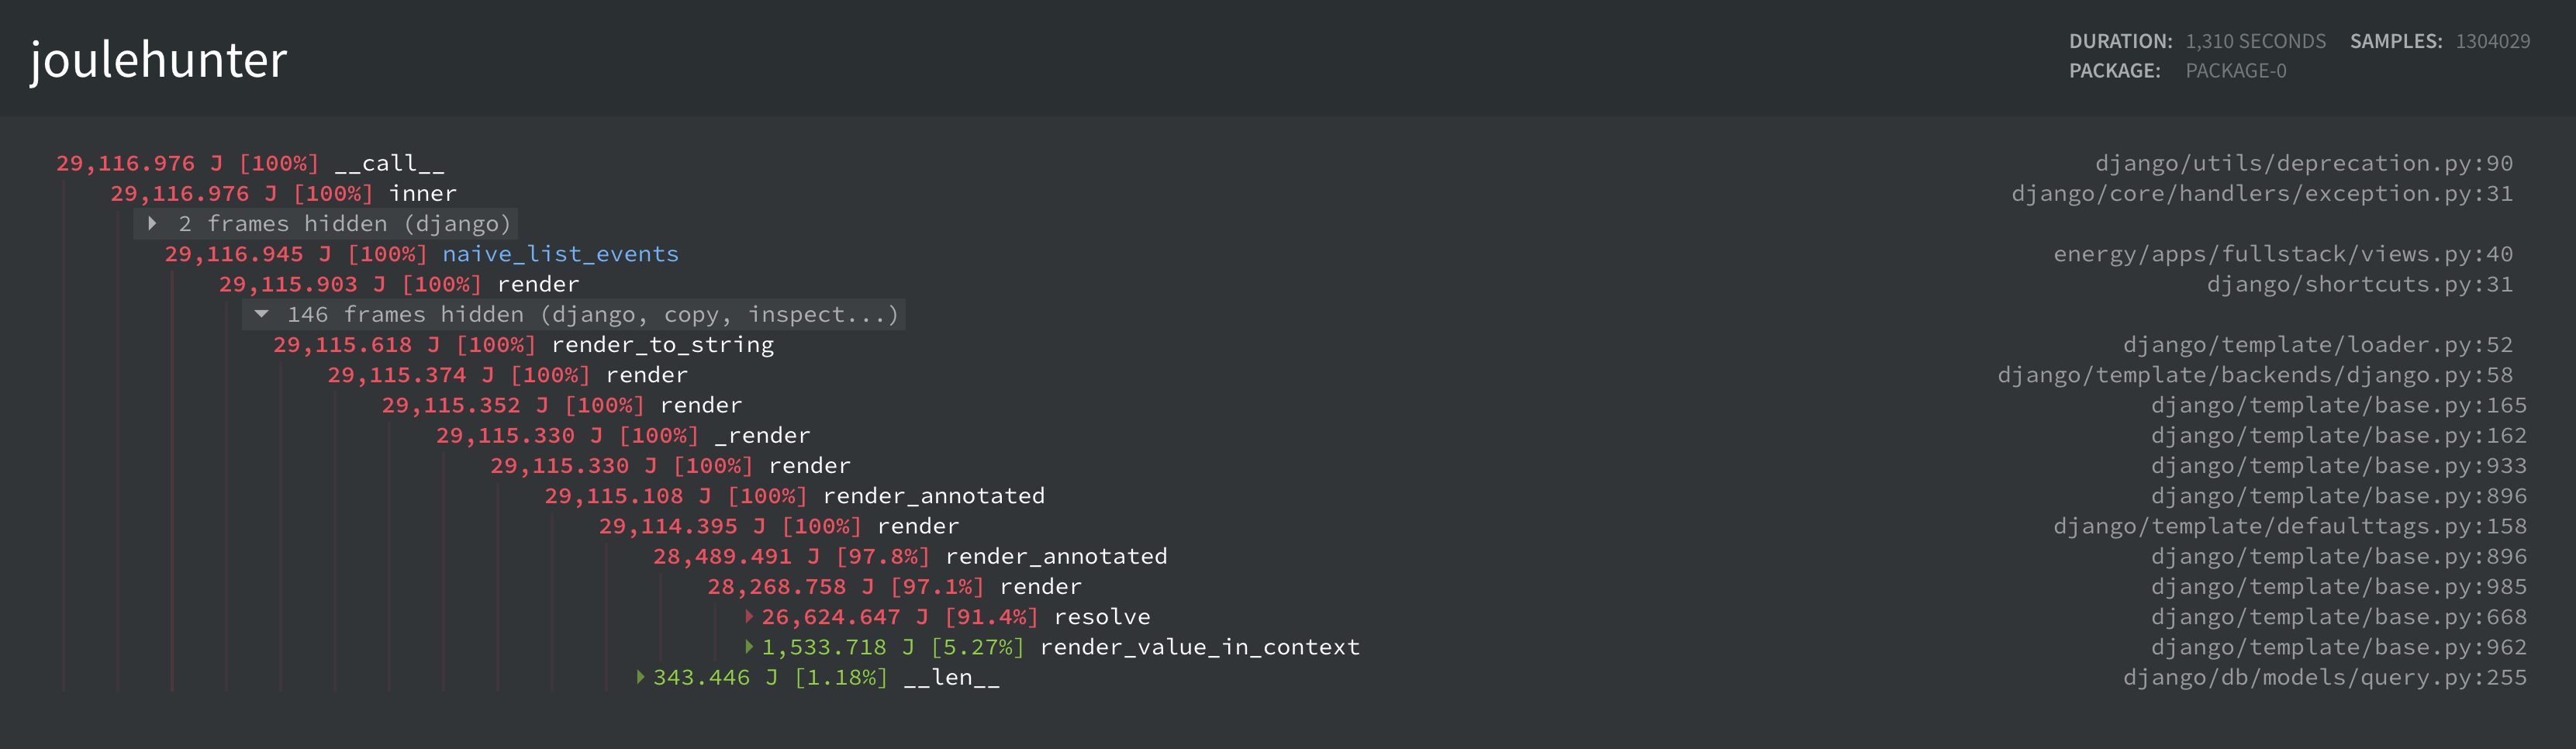
\includegraphics[width=\linewidth]{imgs/django_life_cycle_naive}
    \caption{Tree representation of the energy consumption of a single request in Django (naive version).}
    \label{fig:django_life_cycle_naive}
\end{figure}

%% REMARQUE the experiment with joulehunter isn't conducted within the same machine that is used for generating the boxplot graphs 
% We have chosen Django as our web framework.
Therefore, we chose to study if the choice of the database and the ORM impact energy consumption and web application performance.
% \subsection{Experiment \& Results}
To accomplish so, we examined the cost of a single request of the prior website using various ways to extract data from the database.
We considered using two different databases, \textsc{PostgreSQL} and \textsc{SQlite3}, that store the same records and three different ways to fetch the records:
\begin{enumerate}
    \item \textsf{Vanilla} relies only on the ORM to retrieve the data,
    \item \textsf{Prefetch} queries the data before being requested,
    \item \textsf{Optimized} leverages SQL without passing by the ORM.
\end{enumerate}

As one can observe in \Cref{fig:django}, the strategy to query stored data greatly impacts energy consumption.
As the \textsf{Vanilla} strategy can consume up to $10\times$ more energy than the \textsf{Optimized} one.
Conversely, the choice of the database does not exhibit a key impact on the total energy, despite their different behavior regarding the execution time and the average power.
This can be useful to support developers in choosing which database engine they can adopt, guided by the number of expected requests and the targeted performance.

\begin{figure}[!hbt]
    \centering
    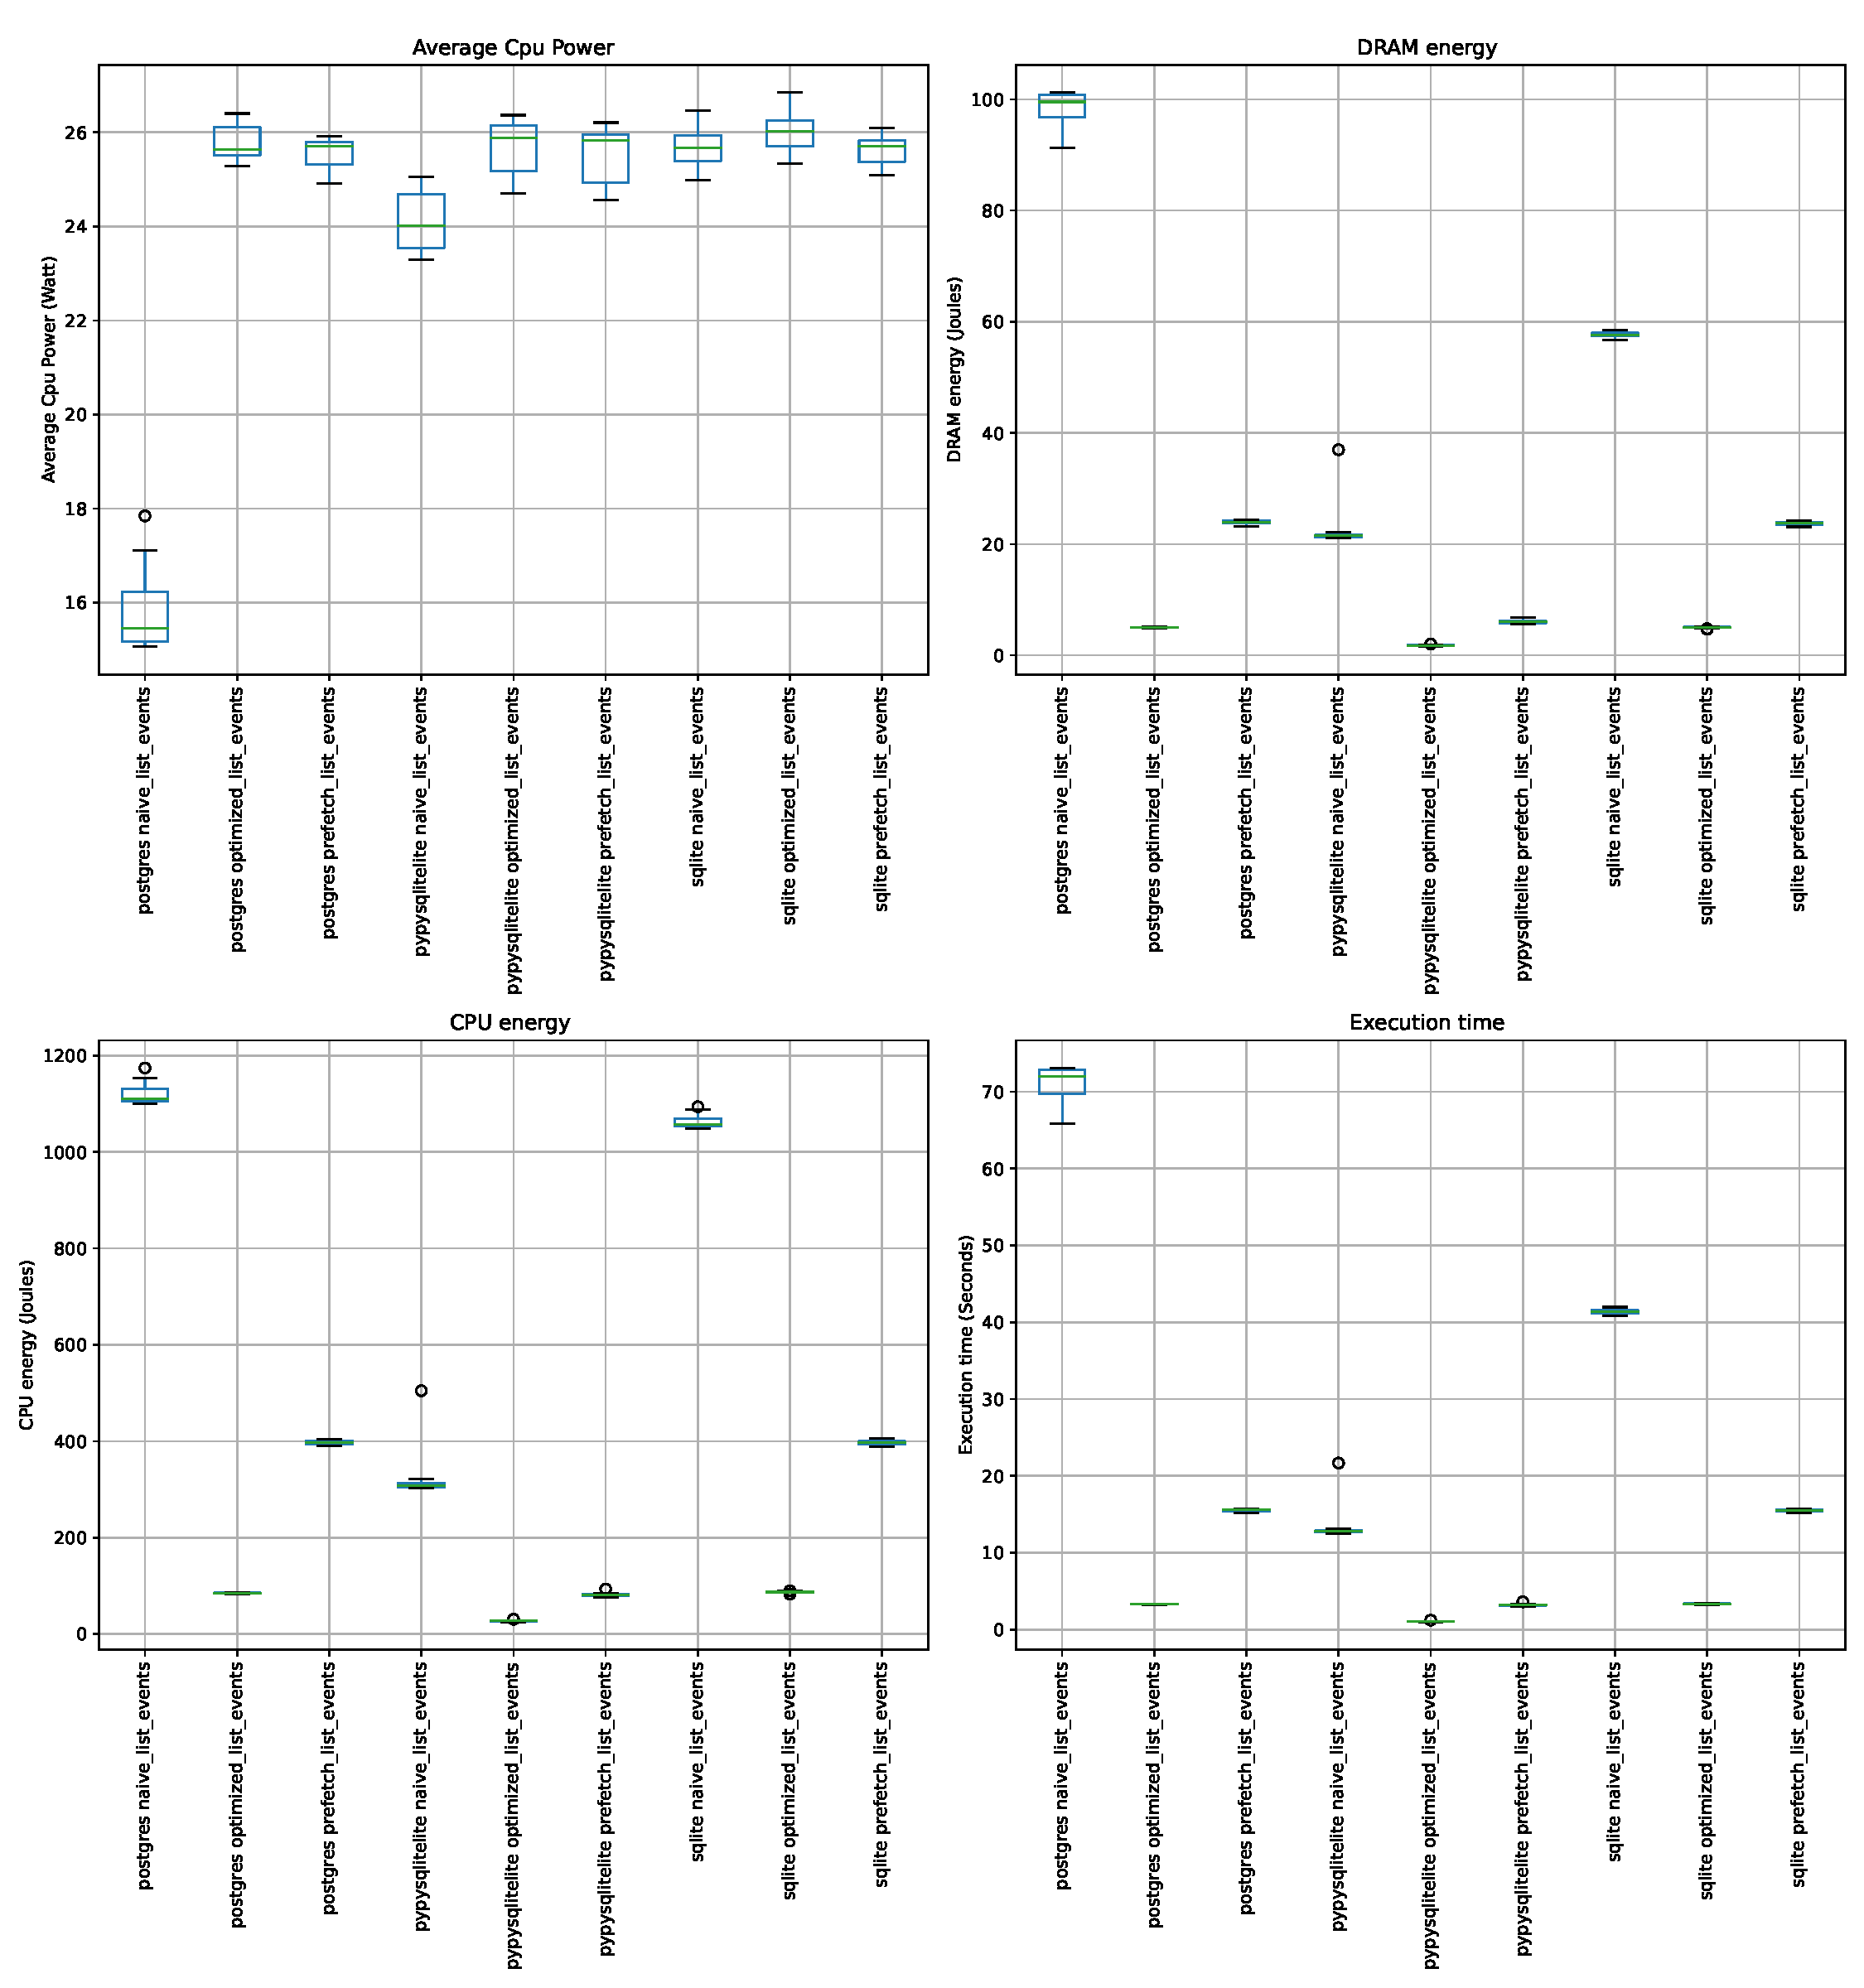
\includegraphics[width=\linewidth]{imgs/django}
    \caption{Key performance indicators observed for different data access strategies.}
    \label{fig:django}
\end{figure}

Another interesting observation is the impact of the interpreter, as \Cref{fig:django} highlights.
For example, using the \textsf{PyPy} interpreter reduces energy consumption, even when adopting the \textsf{Vanilla} strategy.
We will further discuss the choice of Python runtime implementation in the next section.

Finally, we run the same experiment with the \textsf{Optimized} strategy using JouleHunter.
Figure~\ref{fig:django_profiled_optimized} depicts the resulting energy consumption.
As one can notice, while the rendering method consumed the same amount of energy as in the \textsf{Vanilla} strategy (around 1.3\,kJ), the resolve part dropped by $20\times$.

\begin{figure}[!hbt]
    \centering
    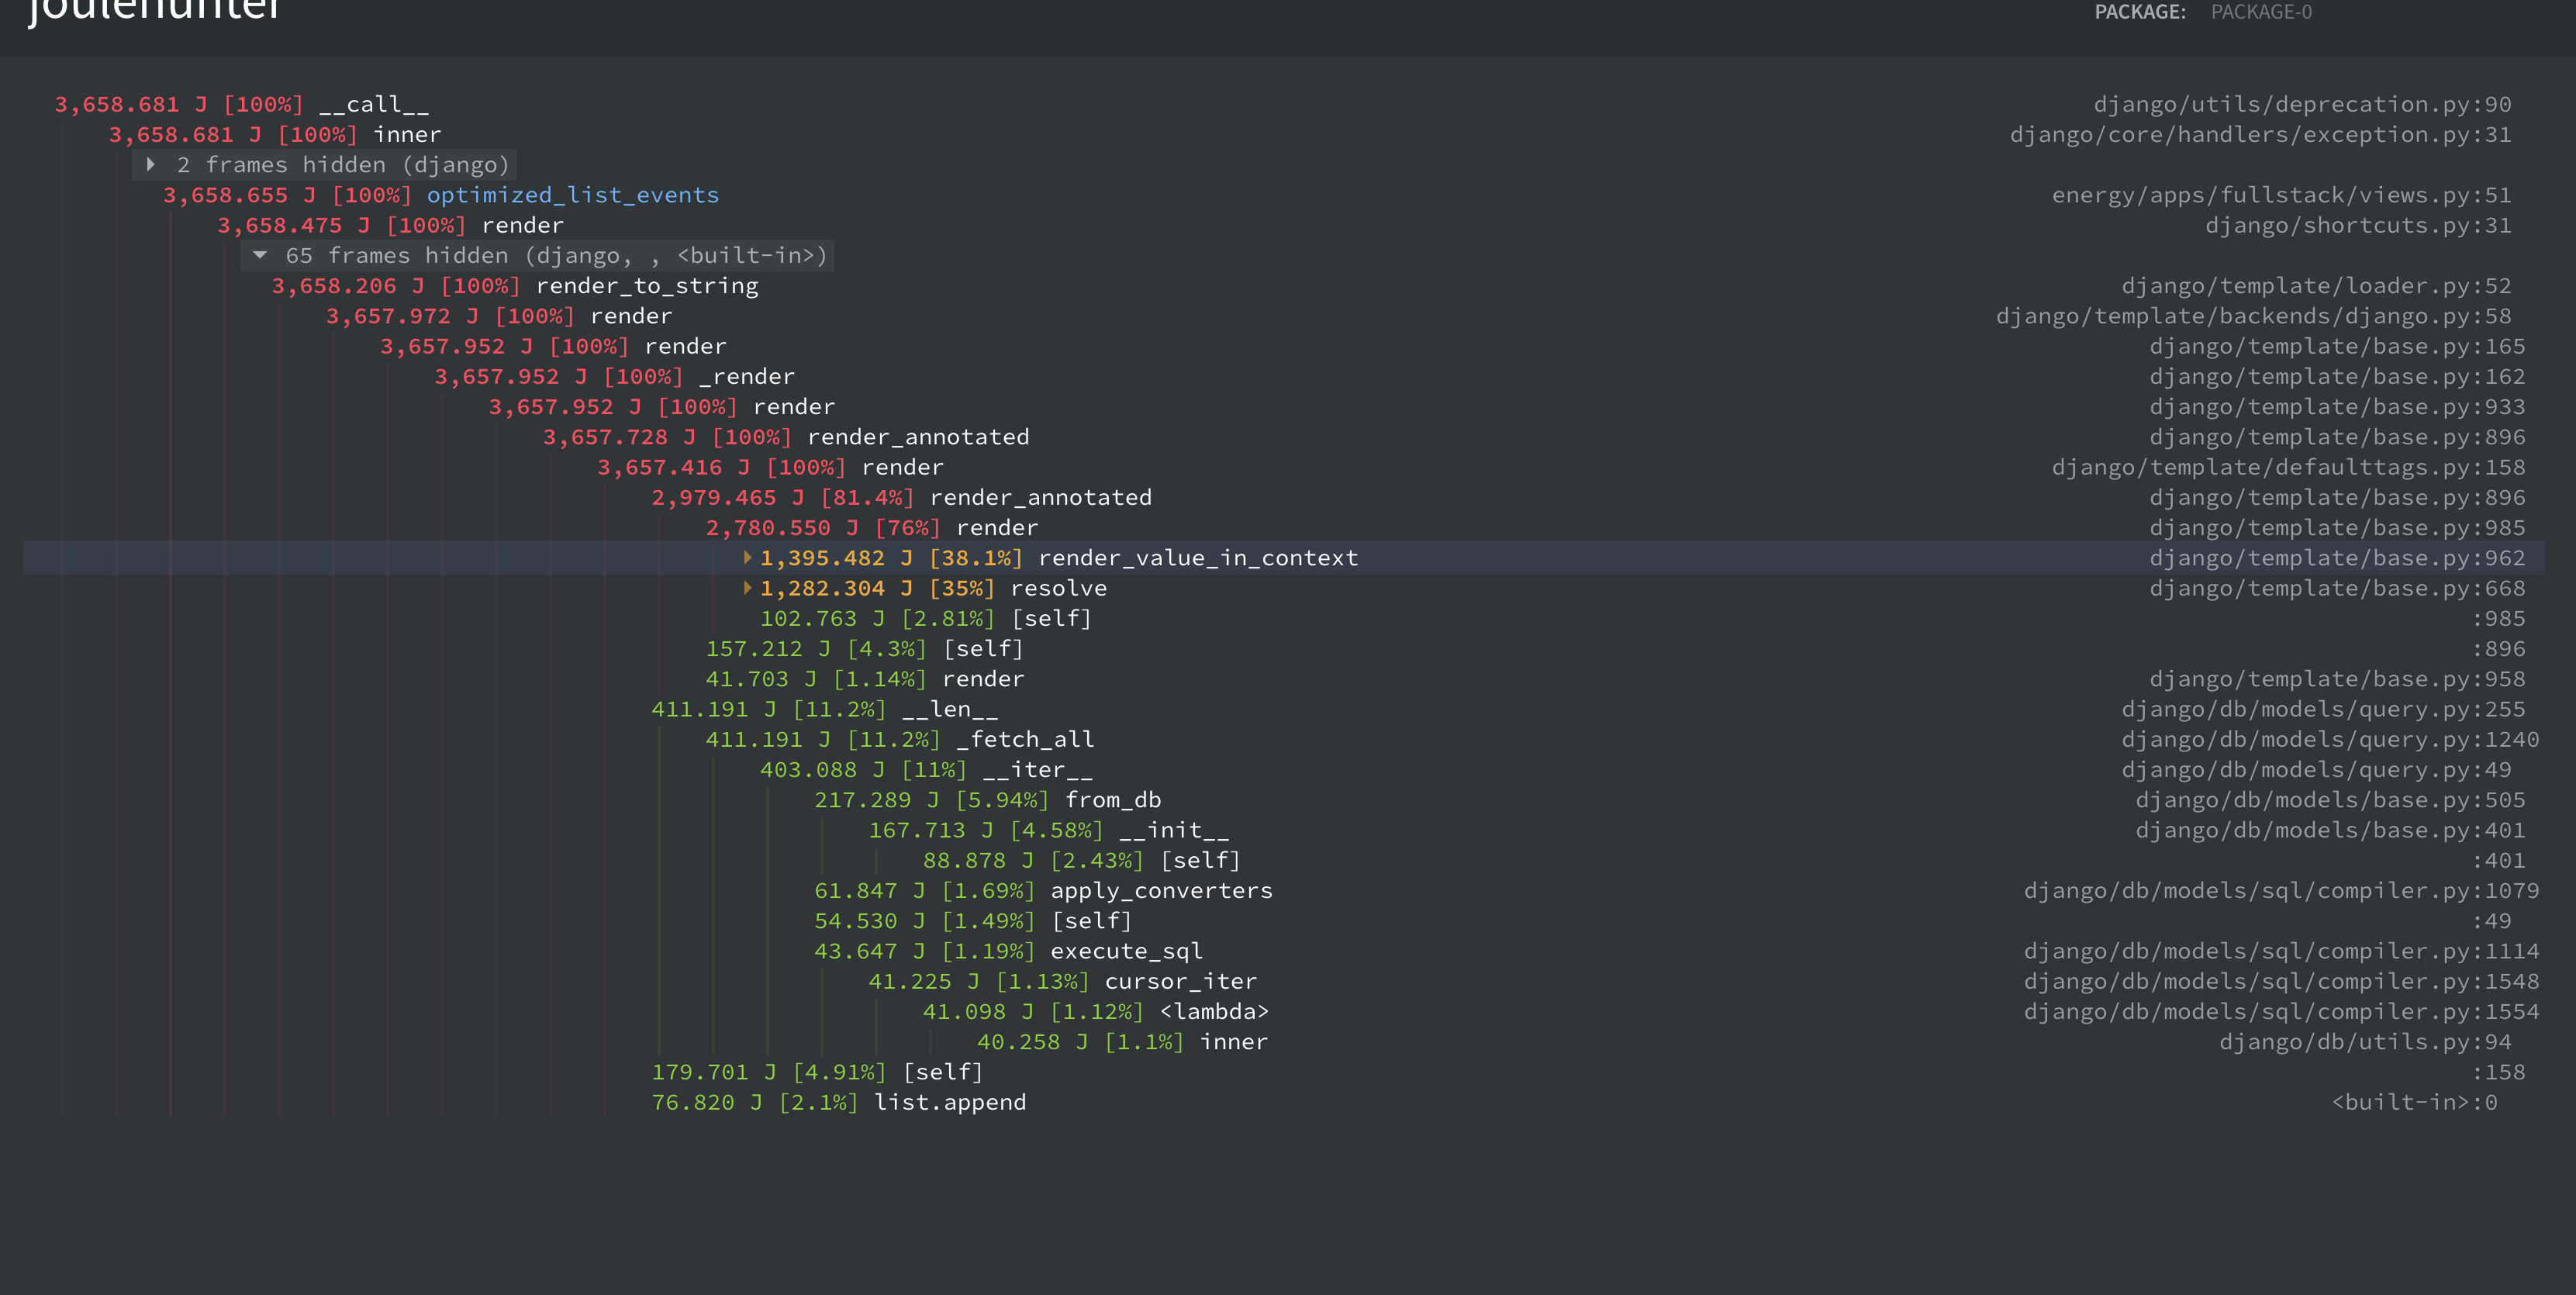
\includegraphics[width=\linewidth]{imgs/django_profiled_optimized}
    \caption{Tree representation of the energy consumption of a request in Django (optimized version)}
    \label{fig:django_profiled_optimized}
\end{figure}

\paragraph{Synthesis}
We can conclude that the database and ORM selection significantly impact the web application performance and energy consumption.
Moreover, unlike rendering responses, many alternatives can be considered to store and query the application database.

\subsection{Python for Data Processing}
Another field of investigation is the type of data and control structures that might impact energy consumption.
In this study, we will run some common algorithms with different data structures and control structures to study if there is any difference in energy consumption.
\subsubsection{Experimental Protocol}
All of the tests in this study are done on the Grid5000 cluster using the same machine, Python interpreter, and library version.
Due to PowerAPI's frequency constraint, we measure the energy of $1,000$ algorithm iterations for each test.
Furthermore, we perform each test 20 times for completeness, deleting the cache between each run.
The data is then averaged and presented in graphs.

\subsubsection{Python Loops}
In the first experiment, we study the impact of the type of loop on energy consumption.
To do so, we execute the following code snippet:
\begin{algorithm}[!htb]
    \begin{algorithmic}[1]
        \State $sum \gets 0$
        \For{$i \gets 0$ to $N$}
        \State $sum \gets sum+1$
        \EndFor
        \State \Return {$sum$}
    \end{algorithmic}
\end{algorithm}

First, the classical \texttt{for(i in range(len(n)))}.
However, as we can see here, unlike other programming languages, it requires extra operations, such as determining the collection length and then using the iterator range.
So, we tried an alternative version: \texttt{for(element in collection)}.
Moreover, in most programming languages, the \texttt{for} loop is translated into a \texttt{while} loop, so we wanted to compare this with a \texttt{while} version.
Therefore, our candidate loops are defined as:
\begin{itemize}[]
    \item \texttt{for (i in range(len(n)))},
    \item \texttt{for (element in collection)},
    \item \texttt{while}.
\end{itemize}

Furthermore, we run the same code snippet for each of these implementations with different primitive data types: \texttt{Int}, \texttt{Float}, and \texttt{String}.

\begin{figure}[!htb]
    \centering
    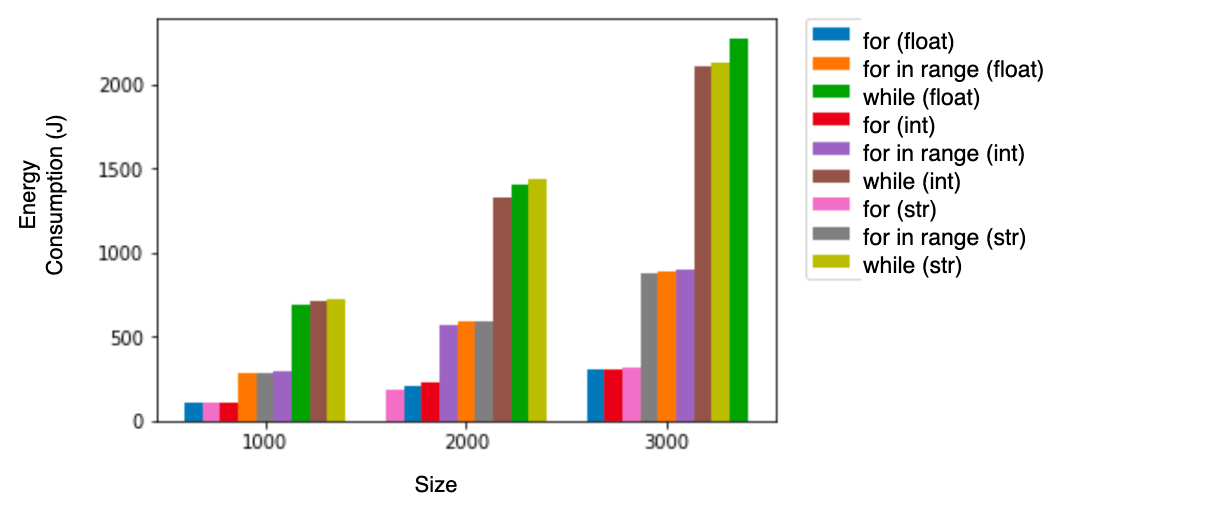
\includegraphics[width=\linewidth]{imgs/python_iterations}
    \caption{Comparison of the energy consumption of different Python loops.}
    \label{fig:pythonloops}
\end{figure}

Figure~\ref{fig:pythonloops} shows the results of the experiment.
As one can notice, the data type has a negligible impact on energy consumption.
However, the way one iterates over the collection has a huge factor.
Interestingly, the \texttt{for in range(...)} loop was by far the optimal one, followed by the regular \texttt{for in collection}, and the \texttt{while} part was the last one with an overhead of 400\% compared to the first option.

The reason behind such behavior is mainly related to how the Python interpreter is implemented.\footnote{\url{https://www.python.org/doc/essays/list2str}},\footnote{\url{https://www.pythonpool.com/for-vs-while-loop-python/}}
Most of the built-in functions and operations are written in C, to reduce the latency of Python applications, and the same goes for the function \texttt{range}.\footnote{\url{ http://python-history.blogspot.com/2010/06/from-list-comprehensions-to-generator.html?m=1}}
Furthermore, the function \texttt{len} has a complexity of $\mathcal{O}(1)$, as it is based on the function \texttt{Py\_SIZE} of C, which stores the length in a field for the object~\footnote{\url{https://wiki.python.org/moin/TimeComplexity}}.
Therefore, the \texttt{for in range(...)} is creating a new iterator that has the same length as the first one and, for each iteration, requires second access (\texttt{l[i]}) instead of one---explaining the doubled time.
The \texttt{while} is even slower due to the implicit increment of the variable, which causes an extra operation during the loop.

To confirm this hypothesis, we tried to construct a new list by editing the elements of the previous one (cf. \Cref{fig:pythontreatement}).
We used four different methods to do so: \texttt{comprehension list}, \texttt{while loop}, \texttt{a map with predefined function}, and \texttt{a map with an anonymous function}.
A comprehension list is a Pythonic way to create a new list by applying a function to each element of the previous one.
It is based on the mathematical set-builder notation~\cite{editiondiscrete}.
The map function is a higher-order function that applies a given function to each collection element.
It is also possible to use an anonymous function, which is a function that is not bound to a name but only to its definition, which in the Python case is called a lambda function/expression.

As one can notice in~\Cref{fig:pythontreatement}, the built-in methods are the most energy-saving ones, while the customize \texttt{while} loop is the heaviest.
Moreover, when increasing the collection size, the map with lambda functions tends to consume less energy than the predefined one.
The reason behind such behavior is that Python treats these functions as local variables, unlike the predefined ones, which are global in our case.
Therefore, they are faster and consume less energy.

\begin{figure}
    \centering
    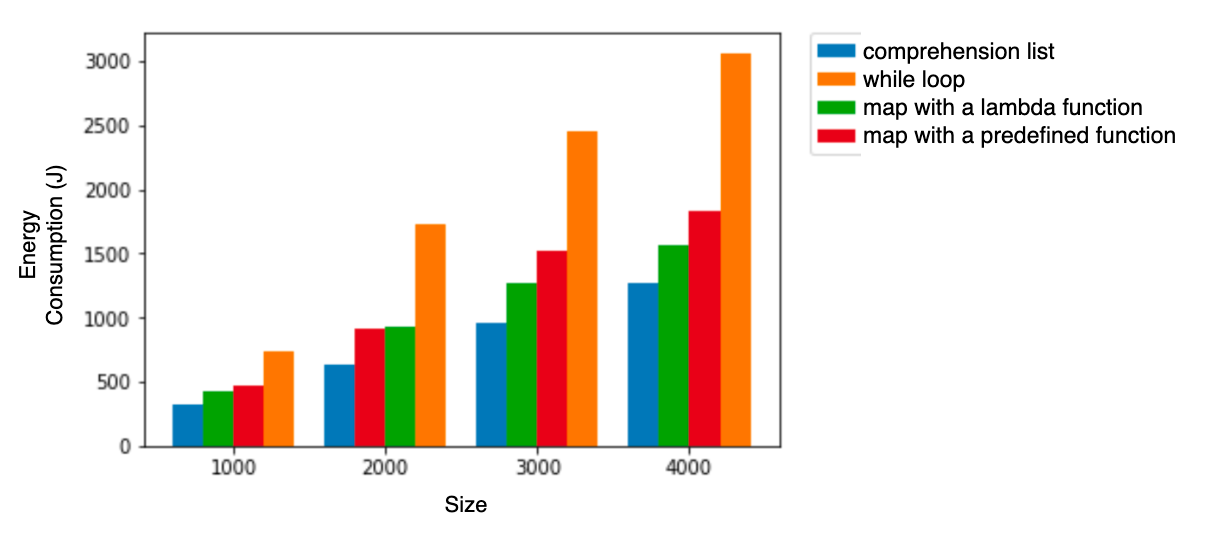
\includegraphics[width=.9\linewidth]{imgs/python_treatemens}
    \caption{Comparison of the energy consumption of different methods to convert a list.}
    \label{fig:pythontreatement}
\end{figure}


\paragraph*{Synthesis}
This study demonstrates that the optimal way to reduce the energy consumption of Python applications is to follow the guidelines and privilege the built-in functions.


\subsubsection{Python \& Multiprocessing}
The purpose of this part is to study the impact of concurrency on energy consumption for Python applications.
To do so, we run a simple code snippet that computes the sum of the first $N$ numbers using the standard concurrency libraries \texttt{multiprocessing~\footnote{\url{https://docs.python.org/3/library/multiprocessing.html}}} and \texttt{multihtreading~\footnote{\url{https://docs.python.org/3/library/threading.html}}}.
We run the following strategies using a Desktop machine with Intel(R) Core(TM) i7-4800MQ CPU @ 2.70GHz with four cores and four hyper-threads.
%  N ==5e5
\begin{itemize}
    \item \textsf{Sequential}: we compute the sum of the first $N$ numbers with no concurency;
    \item \textsf{Multithreading}: we use the \texttt{ThreadPoolExecutor} library to compute the sum of the first $N$ numbers. We divide $N$ by the number of threads, and each thread will compute the sum of the numbers in its range. For our case, we used four threads;
    \item \textsf{Multiprocessing}: we use the \texttt{ProcessPoolExecutor} library to compute the sum of the first $N$ numbers. We divide $N$ by the number of processes, and each process sums the numbers in its range. In this situation, we considered 2, 4, 8, and 16 processes iteratively.
\end{itemize}

Figure~\ref{fig:python_multiprocessing} shows the results of the experiment regarding four metrics: power, execution time, DRAM energy, and CPU energy.
As one can notice, CPU energy is ten folds higher than DRAM one.
Therefore, we will focus on the CPU for this study.

\begin{figure}[!hbt]
    \centering
    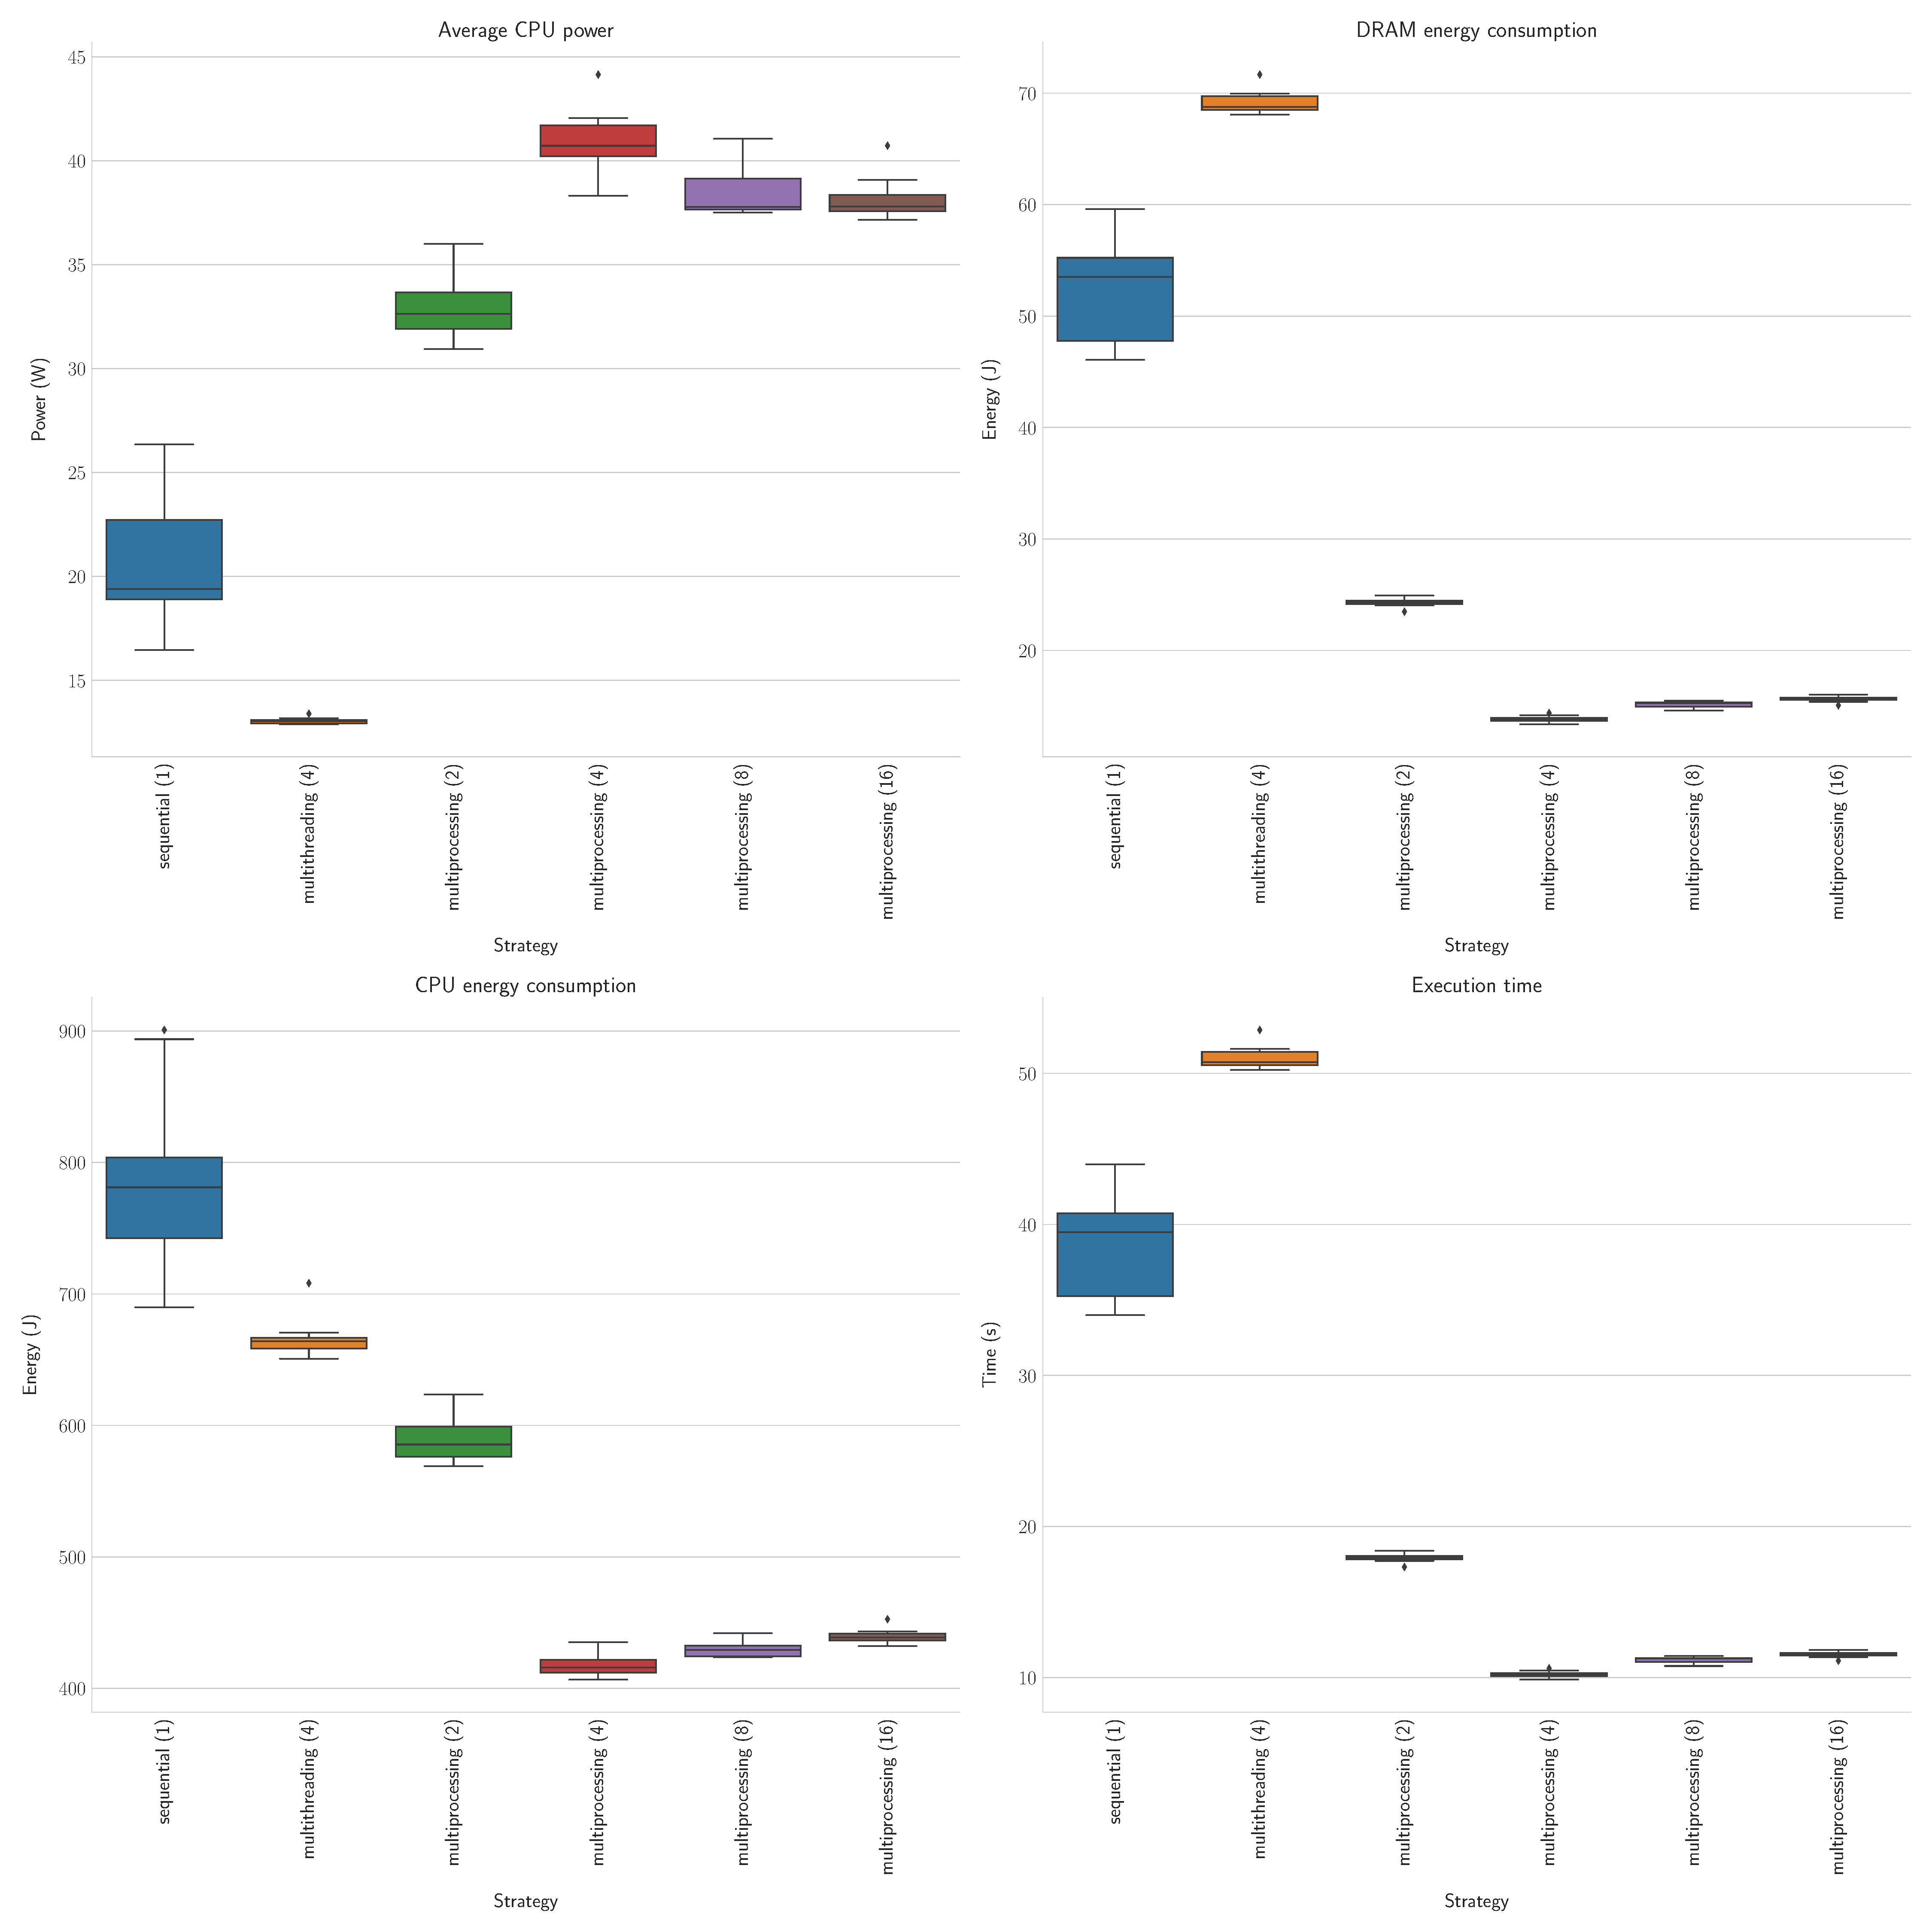
\includegraphics[width=\linewidth]{imgs/python_multiprocessing}
    \caption{Energy consumption resulting from different Python concurrency strategies (number of workers).}
    \label{fig:python_multiprocessing}
\end{figure}

In general, the \textsc{Multiprocessing} strategy is the most energy efficient one, and the fastest one.
However, unexpectedly, the \textsf{Multithreading} option took more time to execute the code snippet than the \textsf{Sequential} one.
Therefore, we will divide our analysis into two parts: the first one will focus on \textsf{Multithreading} versus the \textsf{Sequential} strategies, while the second one will study the behavior of the \textsc{Multiprocessing} strategy.

\paragraph*{Multithreading vs Sequential}
The unexpected behavior of the \textsc{Multiprocessing} strategy is because the Python interpreter is not thread-safe.
Because of the \emph{global lock system} (GLS), Python cannot run multiple threads at the same time.
Therefore, the \textsf{Multithreading} strategy is slower than the \textsf{Sequential} one.
On the other hand, a side effect of this is the context switching between threads, which will put the CPU in a lower power state.
The \textsf{Multithreading} strategy depicts an average power of $13 Watts$ compared to the \textsf{Sequential} one, which is around $22 Watts$.
This difference in power consumption has overcome the lack of performance of the \textsf{Multithreading} strategy, which leads to better energy efficiency.


\paragraph*{Multiprocessing}
Unlike the \textsf{Multithreading} strategy, the \textsc{Multiprocessing} strategy is based on forking the program into multiple processes, which are independent of each other. 
This allows the Python interpreter to run multiple processes simultaneously, hence explaining the better performance of the multi-processing strategy.
However, this will increase the average power consumption of the CPU, which is around $40 Watts$, compared to the \textsf{Sequential} one, which is around $22 Watts$.
Nevertheless, the \textsc{Multiprocessing} strategy is still the most energy-efficient one.

Although increasing the number of processes will reduce the execution time because we split the tasks on the number of processes, there is a point where the execution time increases.
As one can see in \Cref{fig:python_multiprocessing}, the energy consumption correlates with the number of processes until the limit of physical cores, when concurrent processes compete for the CPU.

Before reaching the limit of physical cores, we also observe that the operating system's scheduler tends to favor the execution of processes on the same physical core by taking advantage of the hyper-thread feature.
While this strategy aims to save energy by leveraging the ACPI P-states and C-states of unallocated cores, this leads to increased execution times.

\paragraph*{Synthesis}
This study demonstrates that the optimal way to reduce the energy consumption of Python applications is to adopt the \textsc{Multiprocessing} strategy, which is the most energy-efficient one.
However, this strategy should be used carefully as it can lead to increase power consumption.
This study demonstrates that the optimal number of processes is equal to the number of physical cores, which is four in our case.
When using the \textsf{Multithreading} strategy, it was also found that sometimes the performance of the application has to be given up to save energy.

\clearpage


\section{Python interpreters}\label{sec:pythoninterpreters}

%%% note : add this to the section of python interpreters 
Due to the lack of of support for most of  non conventional pyton interpeters, our main focus was only on micro benchmarks.
Except pypy most of the python implementations don't support extra python libraries, Despite that most of the cases those extra implementations were made to optimize a specific library such as numba with numpy, or intelpython with machine learning algorthms.

\paragraph{preliminary studies}
For the first studies we used only the official version of python. because the goal was mainly to highlight the impact of the structure of code on the energy consumption.
One main inconvienent of the previous methode to reduce the energy consumption, is the hard work that should be done in order to alter the existing code base in order to redcue the energy consumption. To avoid such hustle we tried to find a non intrusive way to make the python code more ecofriendly without changing its structure. One aspect of python is the fact that it is an interptered language which led many works to create their own implementation of the interpeter to enhance one or many aspect of the python code. in the following section we will discuss the impact of those implementations on the energy consumption of python programs, and in which case, one should use a non conventional interpter to save the energy consumption of their program.

To do so, we gathered a list of interpeters, transpilers and some optimization libraries.

the following list, presents the most famous ones .
% We should explain the methodology we used to select these

\begin{enumerate}
    \item \textbf{CPython}:\footnote{\url{https://www.python.org/}} a Python interpreter written in C programming language. It is the reference interpreter of Python. CPython compiles the source code into a bytecode and then interprets it. The CPython project still supports both versions of Python 2 and 3;
    \item \textbf{PyPy}:\footnote{\url{http://pypy.org}} An alternative implementation of the Python interpreter. It is written using \emph{RPython} in order to use the JIT. It compiles the most used portions of the Python code into a binary code for better performance. To benefit from these optimizations, the program has to be executed for at least for few seconds so the JIT has enough time to warm up, the JIT optimization will be applied only the code written by the programmer and not external libraries;
    \item \textbf{Cython}:\footnote{\url{https://github.com/cython/cython}} a static compiler for Python. It translates the Python code into a C code, and then compiles it using a C compiler. It also support(s) an extended version of the Python language that allows programmers to call \emph{C functions}, declare \emph{C types} and use static types which will help the translation of Python objects into native types, such as integers, float, which often means a better performances, since native C libraries are almost all the time faster than the python written once~\cite{pereira_energy_2017}.
    \item \textbf{Intel\,Python}:\footnote{\url{https://software.intel.com/en-us/distribution-for-python}} A customized interpreter developed by Intel in order to enhance performances of Python programs. It is dedicated to data sciences, high-Performance computing. It uses some Intel kernel libraries, such as Math Kernel Library (Intel MKL\footnote{\url{https://software.intel.com/en-us/mkl}}) and data analytics acceleration library (Intel DAAL\footnote{\url{https://software.intel.com/en-us/intel-daal}}). It supports both versions of Python;
    \item \textbf{Active\,Python}:\footnote{\url{https://www.activestate.com/products/activepython/}} developed by the Activestates company, it provides a standardized Python distribution to ensure license compliance, security, compatibility and performance. Therefore, ActivePython has its own built-in packages (more than 300 packages) and supports both versions of Python;
    \item \textbf{IronPython}:\footnote{\url{https://ironpython.net}} A .Net-based Python interpretation platform written in C\# in order to be used over the .Net vm or mono, it benefits from all the optimizations of .Net virtual machine, such as the JIT and garbage collector mechanisms.
    \item \textbf{GraalPython}:\footnote{\url{https://github.com/graalvm/graalpython/}} A Python interpreter that is based on GraalVM \footnote{\url{https://www.graalvm.org/docs/why-graal/}} (a universal virtual machine developed by oracle for running applications written in different programming languages). For the time being, it only supports Python~3 and it is still in the experimental stage;
    \item \textbf{Jython}:\footnote{\url{https://jython.github.io}} Implementation of Python programming language written in Java for the \emph{Java virtual machine} (JVM). Similar to IronPython and GraalPython, it leverages the optimization mechanisms provided by the JVM to enhance the Python programs;
    \item \textbf{MicroPython}:\footnote{\url{http://micropython.org}} a lightweight Python version dedicated to embedded systems and micro-controllers;
    \item \textbf{Nuitka}:\footnote{\url{http://nuitka.net/pages/overview.html}} a Python compiler written in Python that generates a binary executable from Python code. It translates the Python code into a C program that is then compiled into a binary executable;
    \item \textbf{Numba}:\footnote{\url{https://numba.pydata.org}} a library that includes JIT compiler in order to enhance the performances of Python functions using the industry-standard LLVM compiler library;
    \item \textbf{Shedskin}:\footnote{\url{https://github.com/shedskin/shedskin}} a static transpiler that translates implicitly statically typed python into C++ code.
    \item \textbf{Hope}~\cite{akeret_hope_2015}: a Python library that aims to introduce JIT compiler into the Python code;
    \item \textbf{Parakeet}~\cite{DBLP:conf/hotpar/RubinsteynHWS12}: a runtime accelerator for an array-oriented subset of Python;
    \item \textbf{Stackless\,Python}:\footnote{\url{https://github.com/stackless-dev/stackless/wiki}} an interpreter that focus on enhancing multi-threading programming.
    \item \textbf{Pyjion}:\footnote{\url{https://github.com/microsoft/pyjion}} JIT API for CPython, same purpose as Parakeet and Hope.
    \item \textbf{Pyston}:\footnote{\url{https://blog.pyston.org}} performance-oriented Python implementation built using LLVM and modern JIT techniques. the project is funded by dropbox;
    \item \textbf{Grumpy}:\footnote{\url{https://github.com/google/grumpy}} a source-to-source transpiler that translates the Python code into a Go code that will be compiled to a binary executable. It also offers an interpreter called \emph{grumprun} which can directly execute the Python code. Unfortunately, we cannot use it because the project is already outdated (last commit is in 2017) and it has a lot of limitation in term of supporting the Python language, such as some built-in functions and standard libraries;
    \item \textbf{Psyco}:\footnote{\url{http://psyco.sourceforge.net}} a JIT compiler for Python;
    \item \textbf{Unladen\,Swallow}:\footnote{\url{https://unladen-swallow.readthedocs.io/en/latest/}} an attempt to (use) LLVM  as  JIT compiler for CPython.
\end{enumerate}


\subsection{Runtime Classification}
Before futher proceeding with the list of candidate runtimes for Python applications, we propose a classification according to several criterions:
\begin{description}
    \item[\bf Type] refers to the category of runtime infrastructure that supports the execution of a Python application. In particular, we consider 3 types of environments: \emph{Interpreter}, \emph{Compiler} and \emph{Library}. \emph{Interpreter} refers to the class of environment that does not require any preprocessing of Python source code. \emph{Compiler} introduces a compilation phase prior to the execution of the application. Finally, \emph{Library} induces some modification of the source code.
    \item[\bf Runtime] refers to the technology supporting the execution of a Python application. This technology can refer to the programming language used to program the interpreter, the target language for a compiler or a library.
    \item[\bf JIT optimisation] refers to the support of \emph{just-in-time} compilation in the runtime infrastructure supporting the execution of the application.
    \item[\bf GC optimisation] refers to the support of \emph{garbage collection} in the runtime infrastructure supporting the execution of the application.
    \item[\bf Python version(s)] refers to the list of Python source code versions supported by the runtime environment.
\end{description}

We should explain the classification of these runtimes

\begin{table}
    \caption{Classification of Python implementations}
    \label{fig:python-classes}
    \center
    \begin{tabular}{|l|c|c|c|c|c|c|}
        \hline
        \multirow{2}{*}{\bf Name} & \multirow{2}{*}{\bf Type} & \multirow{2}{*}{\bf Runtime} & \multicolumn{2}{c|}{\bf Optimisations} & \multicolumn{2}{c|}{\bf Python}                     \\
        % \cline{1-5} 
                                  &                           &                              & {\bf JIT}                              & {\bf GC}                        & {\bf 2} & {\bf 3} \\
        \hline
        \hline
        CPython                   & Interpreter               & C                            & \no                                    & \no                             & \yes    & \yes    \\
        \hline
        Intel\,Python             & Interpreter               & C                            & \no                                    & \no                             & \yes    & \yes    \\
        \hline
        ActivePython              & Interpreter               & C                            & \no                                    & \yes                            & \yes    & \yes    \\
        \hline
        PyPy                      & Interpreter               & Python                       & \yes                                   & \yes                            & \yes    & \yes    \\
        \hline
        IronPython                & Interpreter               & .Net                         & \yes                                   & \yes                            & \yes    & \yes    \\
        \hline
        GraalPython               & Interpreter               & GraalVM                      & \yes                                   & \yes                            & \no     & \yes    \\
        \hline
        Jython                    & Interpreter               & Java                         & \yes                                   & \yes                            & \yes    & \no     \\
        \hline
        Stackless\,Python         & Interpreter               & python                       & \no                                    & \no                             & \yes    & \no     \\
        \hline
        MicroPython               & interpreter               & c                            & \no                                    & \no                             & \no     & \yes    \\
        \hline
        Pyston                    & interpreter               & LLVM                         & \yes                                   & \no                             & \yes    & \no     \\
        \hline
        Unladen\,Swallow          & Interpreter               & LLVM                         & \yes                                   & \no                             & \yes    & \no     \\
        \hline
        Cython                    & Compiler                  & C                            & \no                                    & \no                             & \yes    & \yes    \\
        \hline
        Nuitka                    & Compiler                  & C                            & \no                                    & \no                             & \yes    & \yes    \\
        \hline
        Shedskin                  & Compiler                  & C++                          & \no                                    & \no                             & \yes    & \yes    \\
        \hline
        Grumpy                    & Compiler                  & Go                           & \no                                    & \no                             & \yes    & \yes    \\
        \hline
        Numba                     & Library                   & C                            & \yes                                   & \no                             & \yes    & \yes    \\
        \hline
        Hope                      & Library                   & python                       & \yes                                   & \no                             & \yes    & \yes    \\
        \hline
        Psyco                     & Library                   & python                       & \yes                                   & \no                             & \yes    & \yes    \\
        \hline
        Pyjion                    & Library                   & .NET Core                    & \yes                                   & \no                             & \yes    & \yes    \\
        \hline
        Parakeet                  & library                   & C                            & -                                      & \no                             & \yes    & \no     \\
        \hline
    \end{tabular}
\end{table}



\begin{table}[hbt]
    \caption{Classification of Python implementations}
    \label{fig:pythonimplementations}
    \center
    \begin{tabular}{|l|c|c|c|}
        \hline
        Version  & Interpreter     & Transpiler/Compiler & Jit library \\
        \hline
        \hline
        Python~2 & Cpython2        & Cython2             & Numba 2     \\
        % \cline{2-4} 
                 & Pypy2           & Shesdskin           & Hope        \\
        % \cline{2-4} 
                 & Pytson          & Grumpy              & Parakeet    \\
                 & Ironpython      &                     & Psyco       \\
                 & Jython          &                     & Pyjion      \\
        % &  &  &  \\
                 & Micropython     &                     &             \\
                 & Pysec           &                     &             \\
                 & StacklessPython &                     &             \\
        % \cline{2-4} 
        \hline
        Python~3 & Cpython3        & Nuitka              & Numba3      \\
                 & Pypy3           &                     &             \\
                 & GraalPython     &                     &             \\
        \hline
    \end{tabular}
\end{table}

There are other implementations that we didn't considerate because either the project aborted many years ago or it has a very limited support for python features.
After the collection of those implementation we filtered them. in order to keep only the versions that are still maintained and support most of python features.
and we classified them into 3 categories depending of their integration with the python code.  In the \ref{fig:pythonimplementations} we describe the implementations that we kept and the version of each implementation and its category.


\begin{figure}
    \centering
    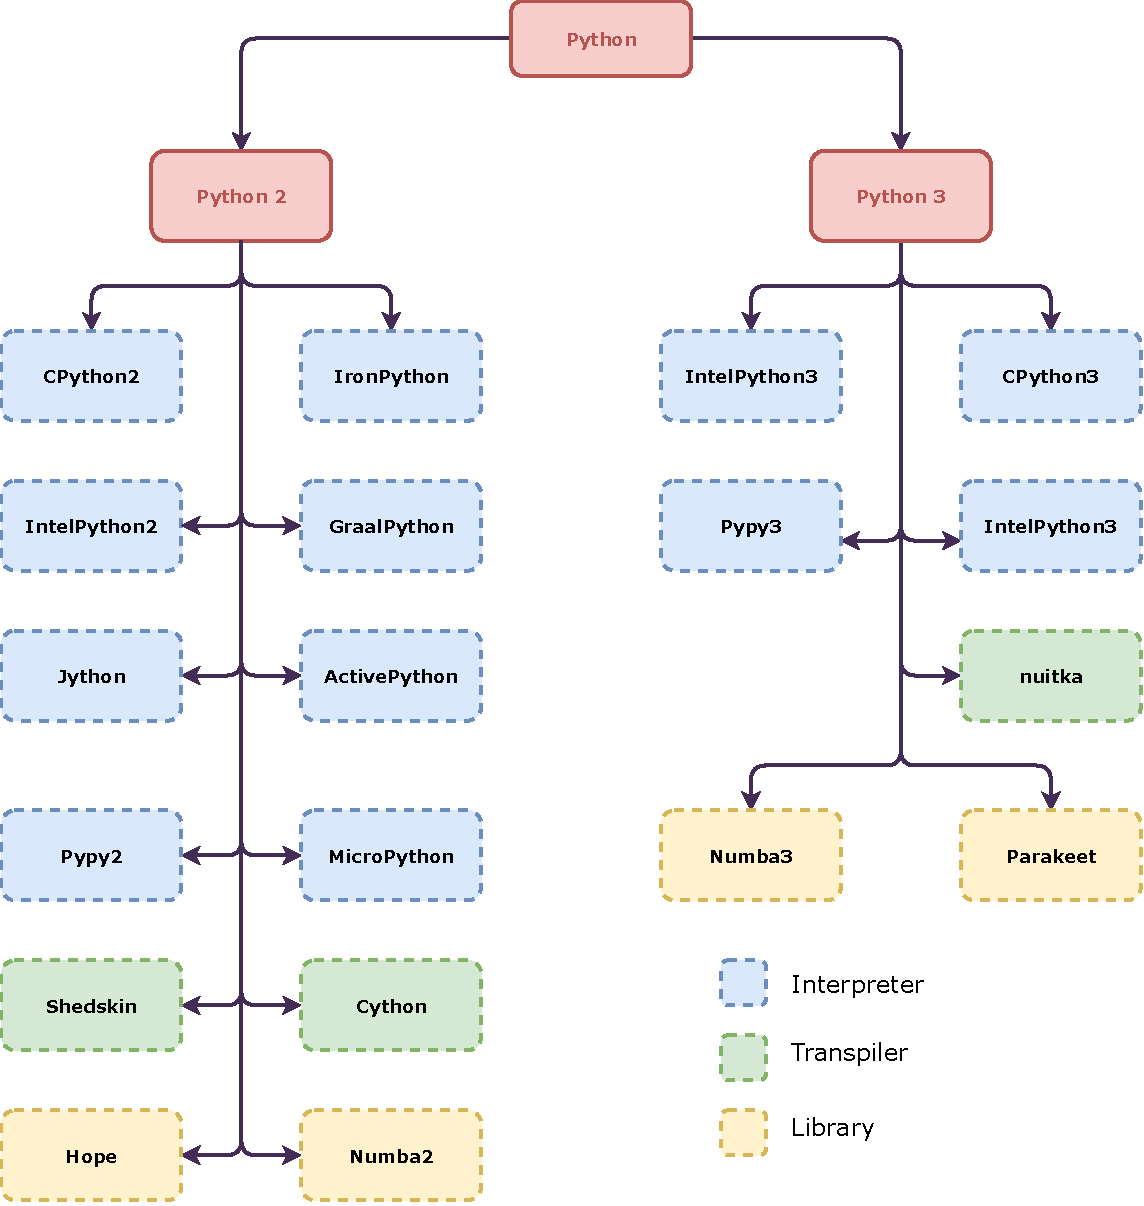
\includegraphics[width=\linewidth]{imgs/python-implementations-tree}
    \caption{Python interpeters}
    \label{fig:interpreters}
\end{figure}



\section{experimetal protocole}

As we have discussed in the previous chapter \ref{chapter:benchmarking}. instead of running the tests, the idea was to design a system that allows practiouners to reproduce and extends our tests. and then we use the same system to run answer some of researchs question.
%%%% probably ill resue the same things from other chapters 
\subsection{measurement context}
\paragraph{Hardware settings}

all our tests have been executed in a Dell PowerEdge C6420 server machine. A summary of its hardware is listed in table \ref{fig:dahuconfig}. The machine is equiped with a minimal version of Debian\,9 (4.9.0 kernel version) where we install Docker (version 18.09.5).



\begin{table}[hbt]
    \begin{tabular}{ll}
        \hline
        CPU     & Intel Xeon Gold 6130 (Skylake, 2.10GHz, 2 CPUs/node, 16 cores/CPU)                                                     \\
        Memory  & 192 GiB                                                                                                                \\
        Storage & 240 GB SSD SATA Samsung MZ7KM240HMHQ0D3                                                                                \\
                & 480 GB SSD SATA Samsung MZ7KM480HMHQ0D3                                                                                \\
                & 4.0 TB HDD SATA Seagate                                                                                                \\
        Network & eth0/enp24s0f0, Ethernet, configured rate: 10 Gbps, model: Intel Ethernet Controller X710 for 10GbE SFP+, driver: i40e \\
                & ib0, Omni-Path, configured rate: 100 Gbps, model: Intel Omni-Path HFI Silicon 100 Series [discrete], driver: hfi1      \\
        \hline
    \end{tabular}
    \caption{Testing Machine Configuration }
    \label{fig:dahuconfig}
\end{table}

\begin{figure}[hbt]
    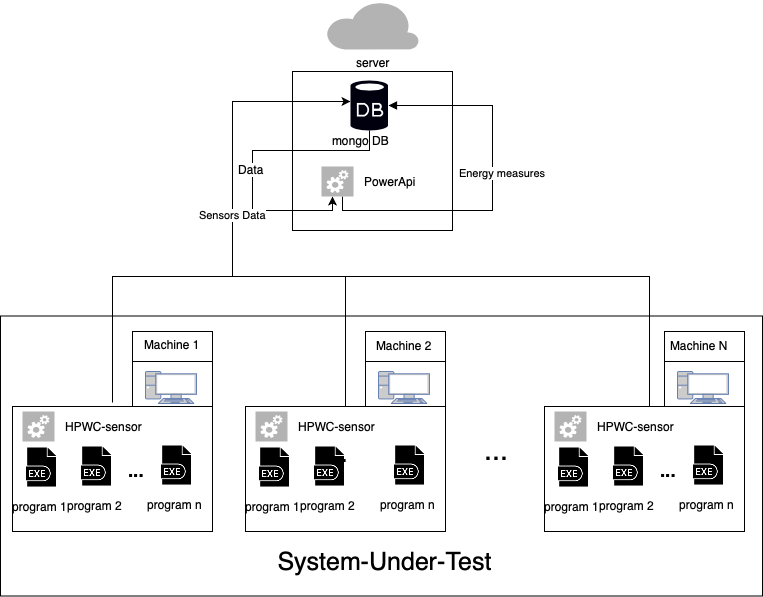
\includegraphics[width=\linewidth]{imgs/SmartWatts.png}
    \caption{powerapi architecture}
    \label{fig:powerapi}
\end{figure}

\paragraph{software settings}
For the sake of reproducibility, each experiment runs within a Docker container.
for each test we create a docker image.
\subsection{Metrics}
Our focus will be mainly on CPU energy consumption because it is ten folds more than the DRAM one, since it is finit job benchmarking, time is highly correlated within the energy, and it will be only useful to explain certain energytical behaviour so we wont put a lot of focus on this metric.

%% basically i what i want to say is that we we care mostly about energy, because there are studies that were made on the performance, plus the DRAM is not that interested even within the heavy memory  benchmakrs 
% TODO : ADD DRAM graphs for vectors and matrix multiply 


\paragraph{Energy measurement}

As we know, the energy of a program is the integrale of its power overtime. For us ower case, we used Intel \emph{Running Power Average Limit} (RAPL)~\cite{Khan:2018:RAE:3199681.3177754} to collect the power samples of the running tests,

We used used \textsc{PowerAPI}~\cite{DBLP:journals/jss/ColmantRKSFS18}, to report Data collected by intel Rapl and send it into another machine that we call computing machine. then we calculate the Energy using  the the trapezoidal rule.


\ref{fig:trapezrule}
\begin{figure}[hbt]
    \centering
    \begin{equation}
        E = \int^a_b P(t)dt \simeq \sum^n_{k=1} \frac{P(t_k-1)+P(t_k)}{2}
    \end{equation}
    \caption{}
    \label{fig:trapezrule}
\end{figure}



figure \ref{fig:powerapi} shows the architecture of our testing model.


The reason of separation between data collection and energy calculation is to minimise any interference with the test so our sensor is a light c program running inside a docker container.
\subsection{tests preparation}



To study the behaviour of the python implementation regarding the energy consumption, we have to focus on the effect of the implementation and mitigate the maximum any side effects such as the organisation of the code or any extra consumption due to the operating system or tier libraries.
Therefore, for each test we took the implementation written in python2 as a reference and tried to use it in other implementations as it is. If it is not supported by python3, we transformed the code using the officiel library  \emph{2to3}\footnote{\url{https://docs.python.org/3.7/library/2to3.html}}.
In the case of the libraries that use \emph{JIT} adding a decorator to the function that we want to optimize was enough, if there are other changes we assume that they alter the original code which is against our purpose.

Each test is implemented in a Docker container for the several reasons
\begin{itemize}
    \item Isolation: each container has only the test program implemented with a single python runtime to remove any interference between different implementations.
    \item Deplpoyment: to use the testing machine without extra configurations that may alter the behaviour of the os toward the enrgy consumtion
    \item Reproductibility: One of the most frequent benchmark crimes~\cite{DBLP:journals/corr/abs-1801-02381} in research is the lack of Reproductibility, by using Docker we ensure that each test has an Image that will be accessible in public.
\end{itemize}

Despite the presence of the official docker images for the most of the runtimes, we prefered to build our own using the same reference image in order to remove any bias due to the Os used in the offical image.We used ArchLinux with the kernel version 4.9.184 as a base image.


\subsection{Extension}
As we have done with the previous chapters. we provide a tool that allows to extend the tests with new workloads and new candidates.
In the repository \footnote{\url{https://github.com/chakib-belgaid/python-implementations}}.
we have a tool that allows to generate new workloads and new candidates.
The script \texttt{generator.py} allows to create new benchmarks by implementing a python code within different interpeters. then it generates \texttt{launcher-benchmark.sh} that can be used directly to run the expermient. Furthermore all the successful implementations are stored in seperate directory and the that couldn't work ( mostly because of compatibility issues) stored in a recap file called \texttt{benchmarkTest.md}. where benchmark is the name of the new workload;
To add extra \textbf{candidates} one should add a base docker file
that containes the new implementation and if there should be extra manipulation that should be added to the workload files ,such as adding new decorator or changing some parameters, then they should be added as an extra function in the script \texttt{generator.py}. Finally they should be included in the python candidates.

\section{Results and finding}



\section{placeholder}
we performed a shapiro normality test for the first on the results, and almost all the p-values smaller than alpha=0.01\%
therefore the distrubution is not normal - which is kinda true because if it was normal then we dont have any comparaison --

for arrays and vectors  graalpython took so much time that we decided to remove it

the startup cost for ironpython was too high
for graalpython and ipy they couldnt handle big numbers hence the overflow  when it comes to execution time
but since we measure the energy outside the values of the energy aren't impacted

as usual there is  correlaction between DRAM and CPU so no need to classify based on DRAM + the DRAM consumes less 10\% of the  energy compared to the CPU

so the plan is to prove that there is a statistical difference
then we use the multiparameter optimization , howerver we stop in the phase where we calculate the score
because we dont know the weight of each parameter ( of tommti microbenchmark) and instead of doing the sum with the coefissients we use the radar plot to let the reader decide which one is the most suitable for his usage. howerver since the differences are gigantics we change the scale to logarithmic to be easier for the eye to read



\begin{figure}
    \caption{energy consumption of different impelementations using Bit Operation benchmarks (Joule) }
    \label{table:bitops}
    \begin{tabular}{lrrrrr}
        \toprule
        benchmark    & A          & GG         & LL         & Or         & XOR        \\
        \midrule
        activepython & 676.980672 & 763.208040 & 651.783048 & 743.016425 & 728.828481 \\
        cpython2     & 441.082298 & 435.886950 & 430.846171 & 415.247383 & 419.081447 \\
        cpython3     & 595.209019 & 685.085315 & 563.839300 & 657.972734 & 655.560574 \\
        cython       & 35.077408  & 182.688395 & 274.177830 & 34.868014  & 34.504778  \\
        nuitka       & 33.260991  & 32.980380  & 33.256450  & 33.472770  & 33.030889  \\
        numba2       & 9.102939   & 8.411176   & 9.460620   & 9.375920   & 9.755952   \\
        numba3       & 9.566646   & 10.144212  & 9.219703   & 9.344613   & 9.665108   \\
        pypy2        & 8.456867   & 7.844918   & 8.286278   & 8.138692   & 7.952999   \\
        pypy3        & 7.552731   & 8.093884   & 8.108508   & 8.669448   & 8.623737   \\
        shedskin     & 8.024198   & 8.070870   & 8.399917   & 8.126236   & 8.277546   \\
        \bottomrule
    \end{tabular}

\end{figure}


\begin{figure}
    \centering
    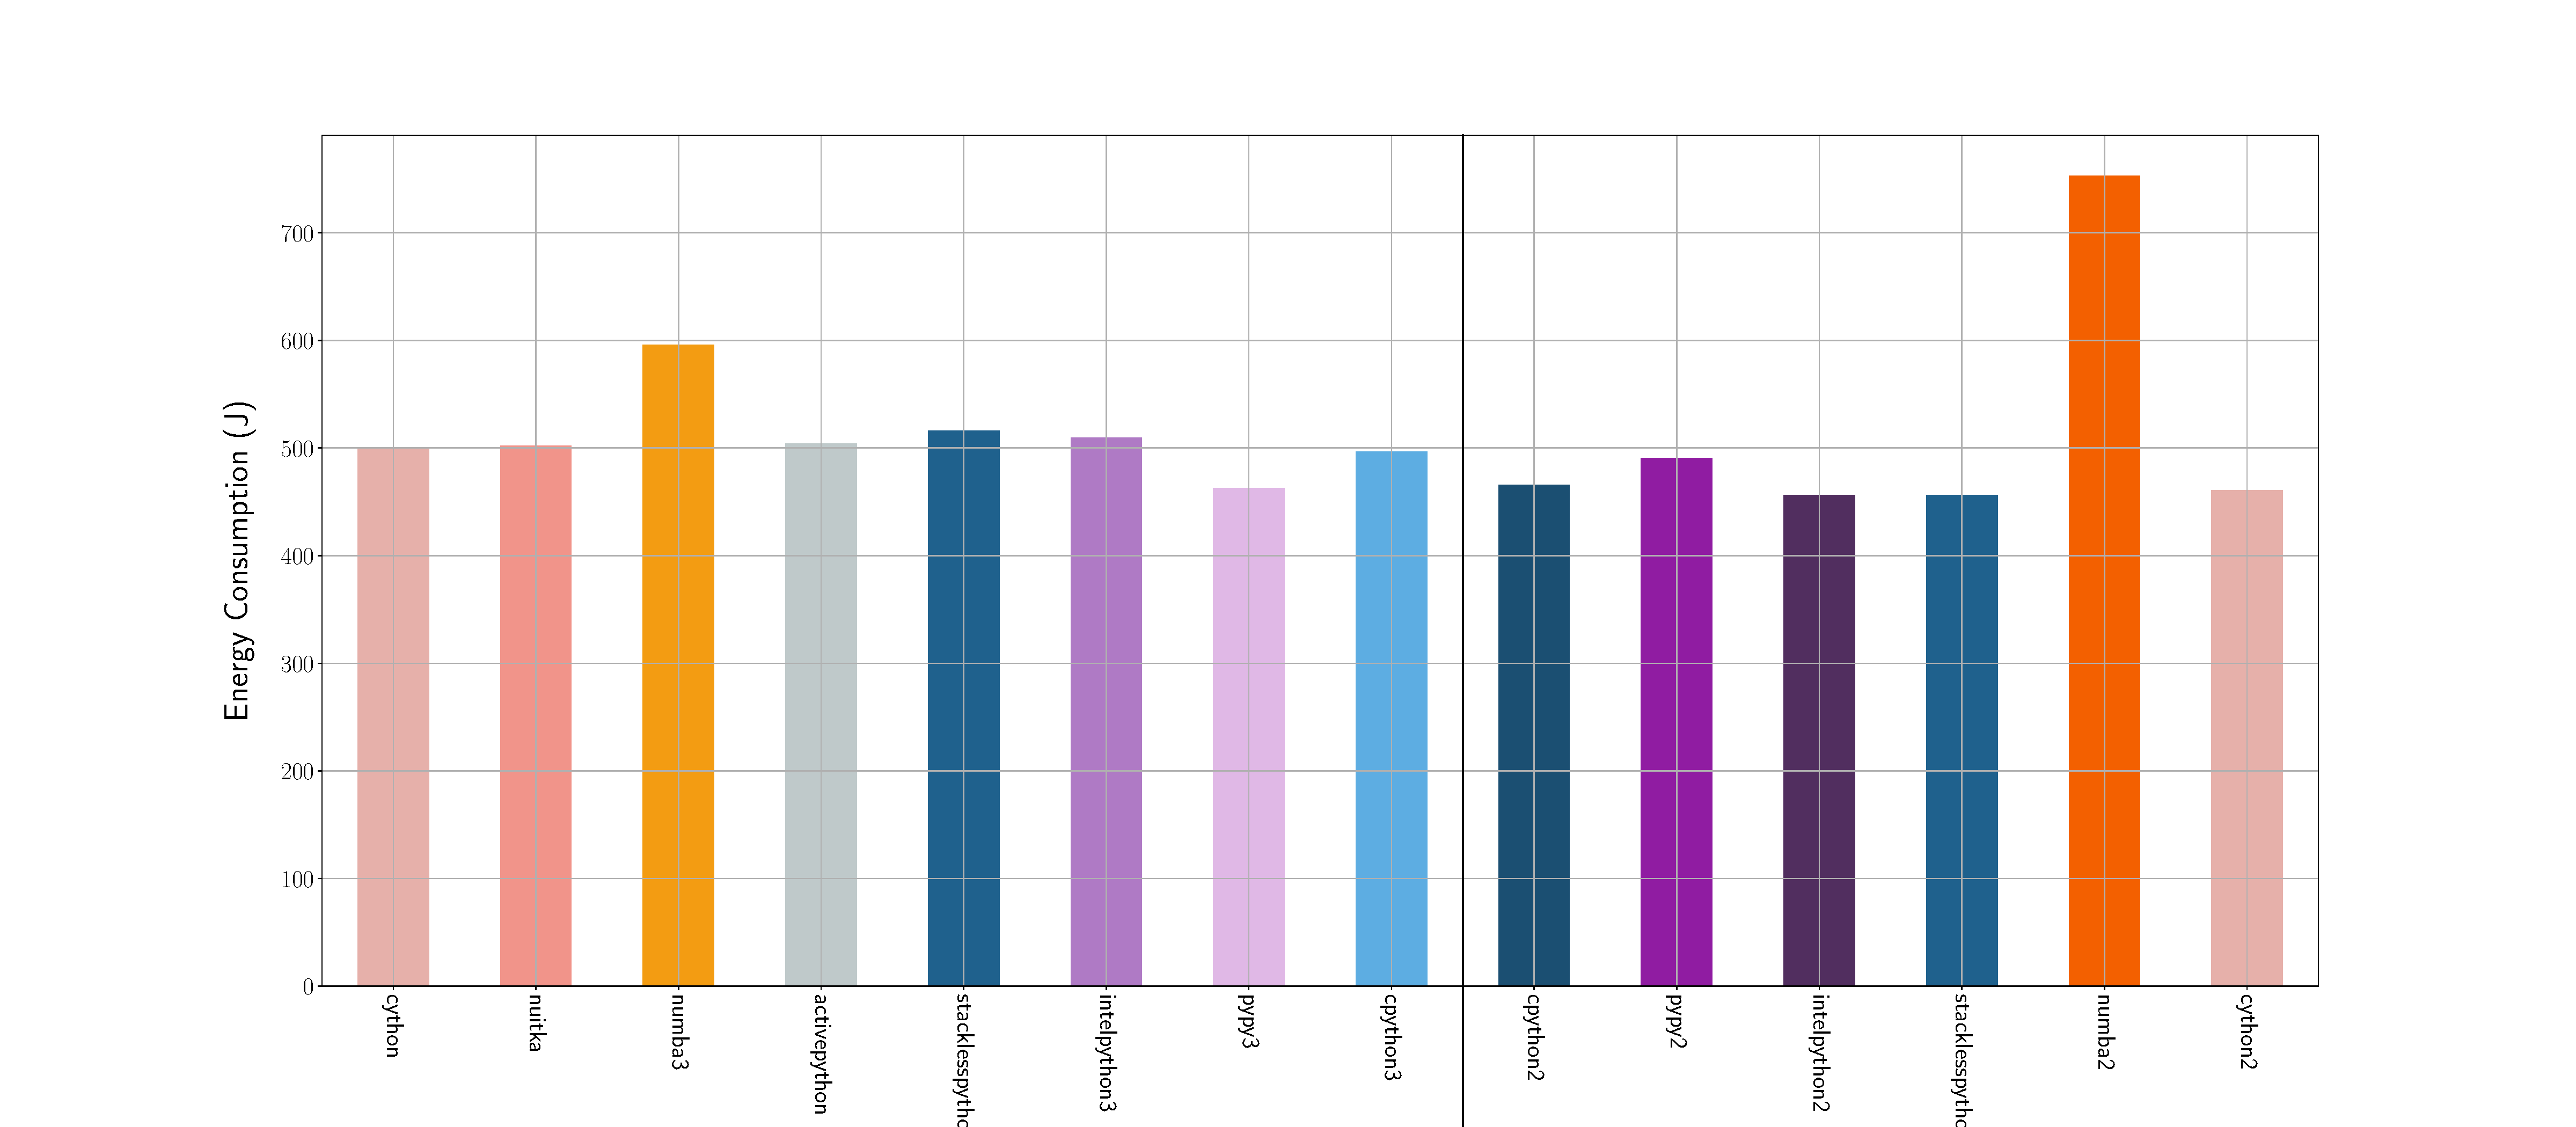
\includegraphics[width=\linewidth]{imgs/barplot_binarry_tree}
    \caption{energy behaviour based on multiprocessing}
    \label{fig:python_multiprocessing}
\end{figure}

\begin{figure}
    \centering
    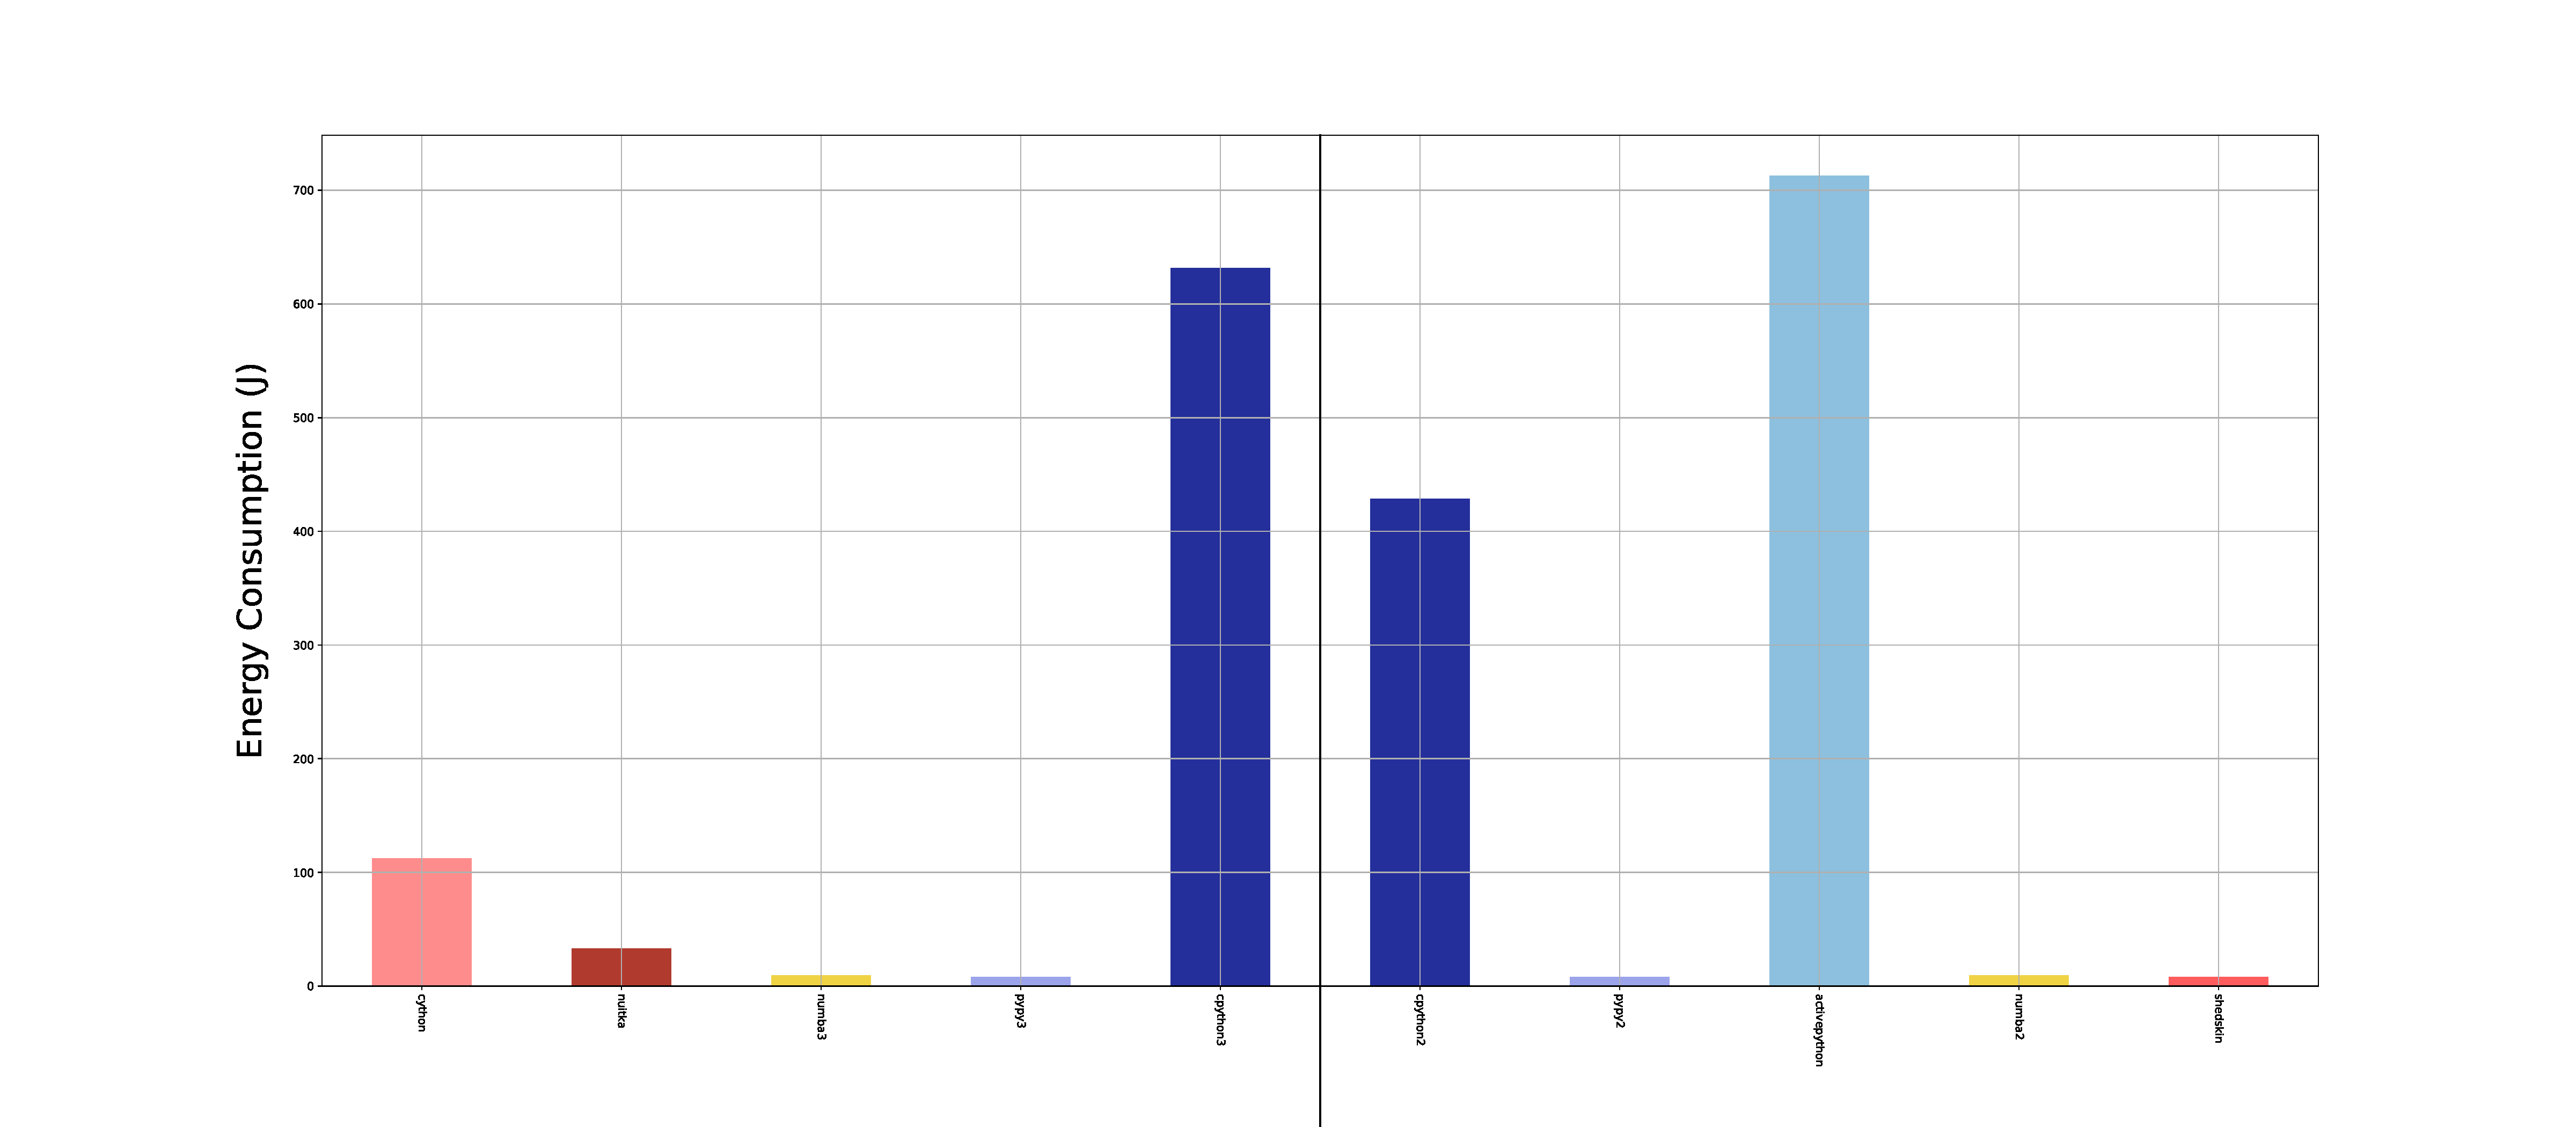
\includegraphics[width=\linewidth]{imgs/bitopts_mean}
    \caption{Mean consumption of different implementations of bit operations (Joule) }
    \label{fig:bitops}
\end{figure}

\begin{figure}
    \centering
    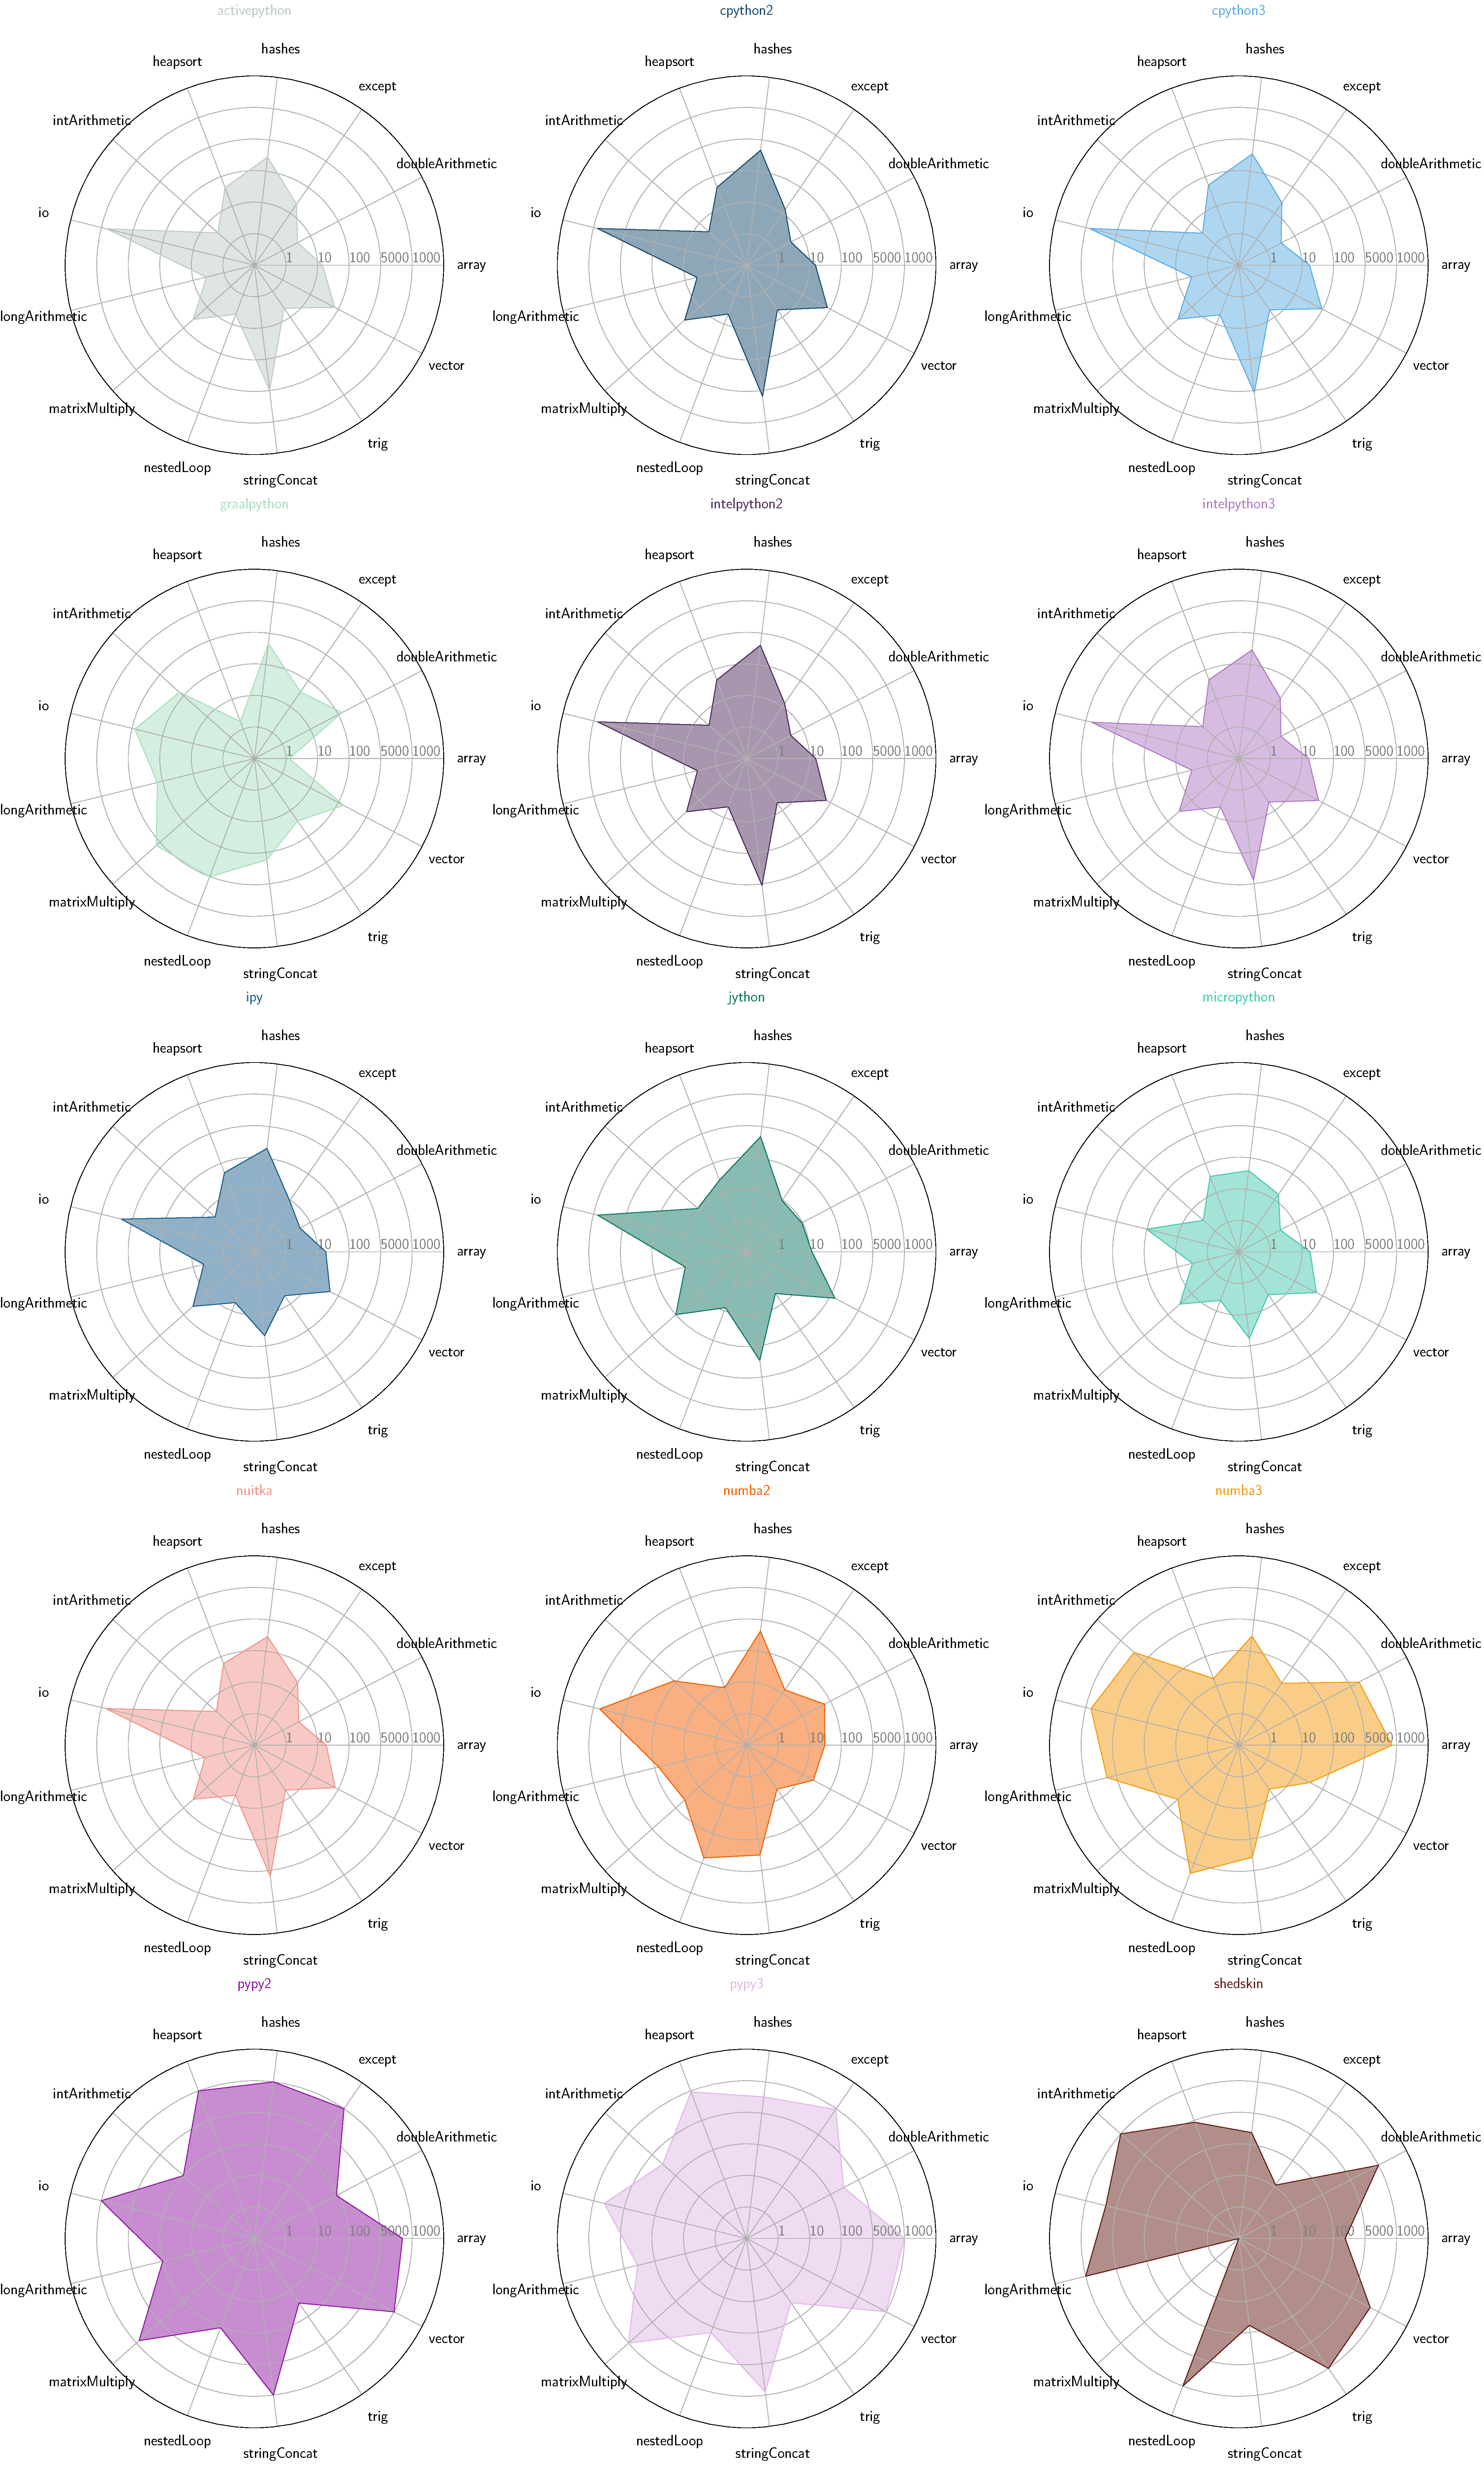
\includegraphics[width=\linewidth]{imgs/alltomti_performance}
    \caption{different interpererts optimisation }
    \label{fig:tommi_all}
\end{figure}
\begin{figure}
    \centering
    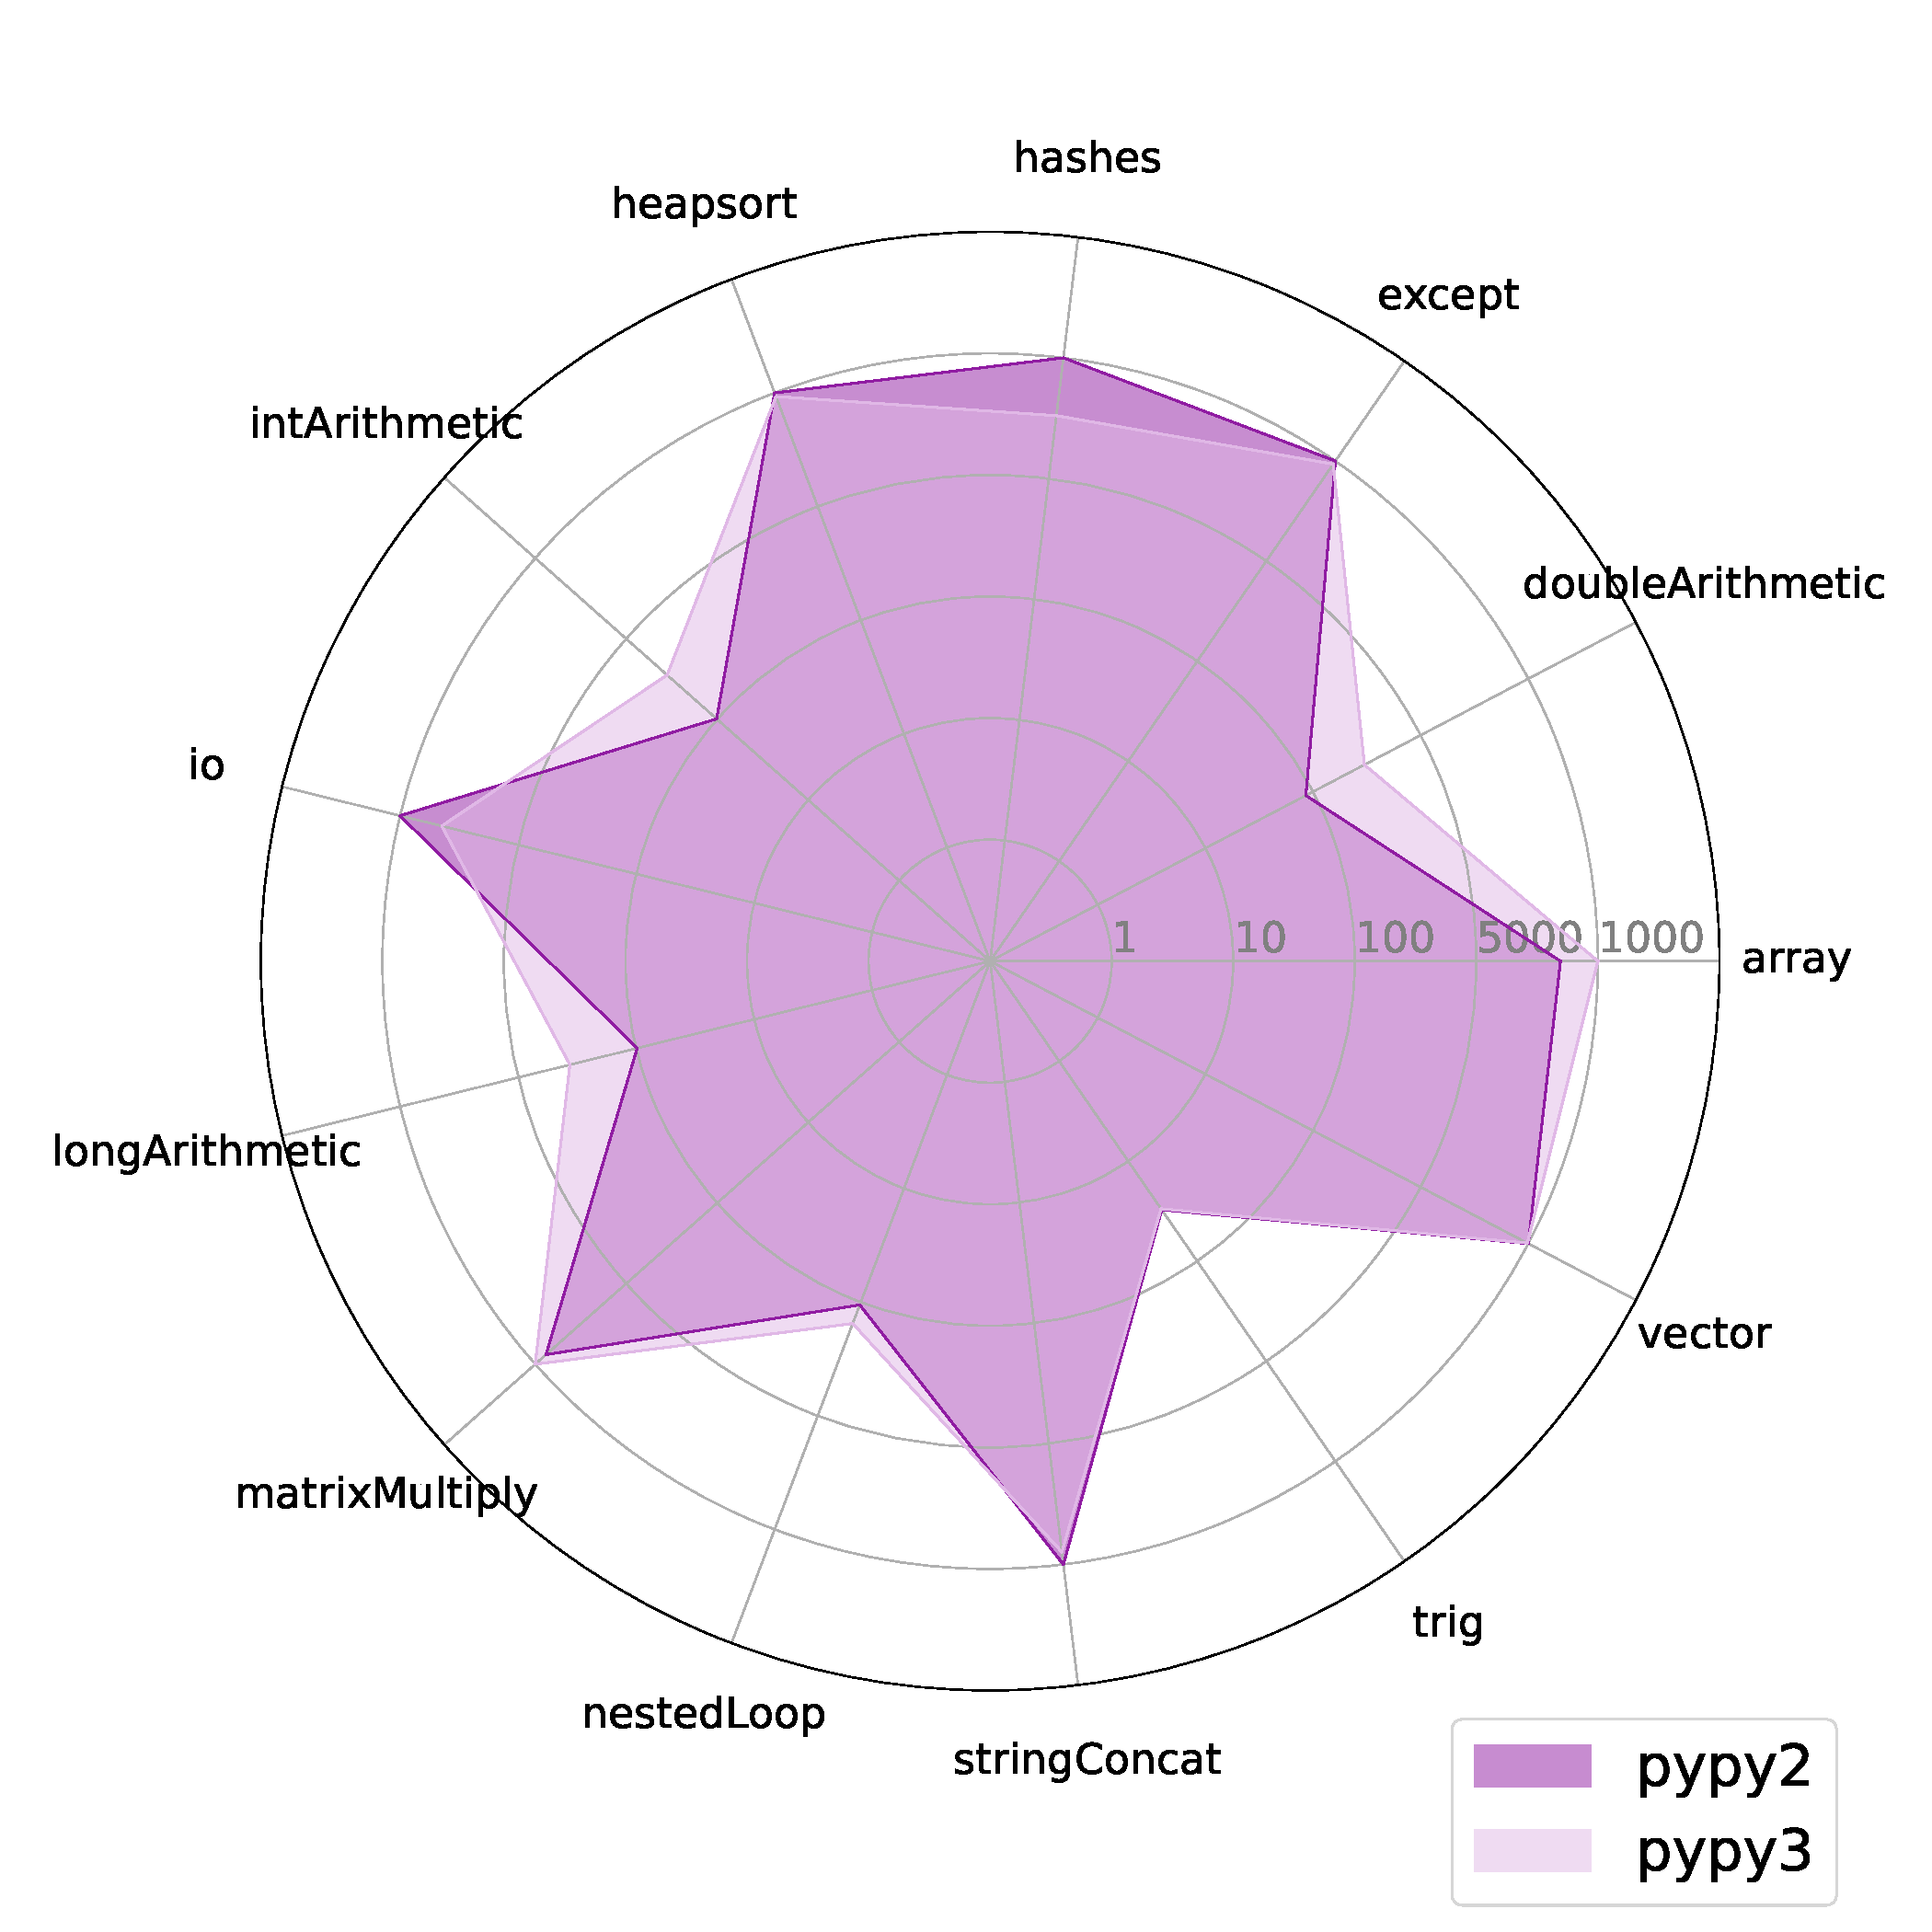
\includegraphics[width=\linewidth]{imgs/tommti_compare__pypy2_pypy3}
    \caption{green factor of pypy }
    \label{fig:pypy2vspypy3}
\end{figure}

\begin{figure}
    \centering
    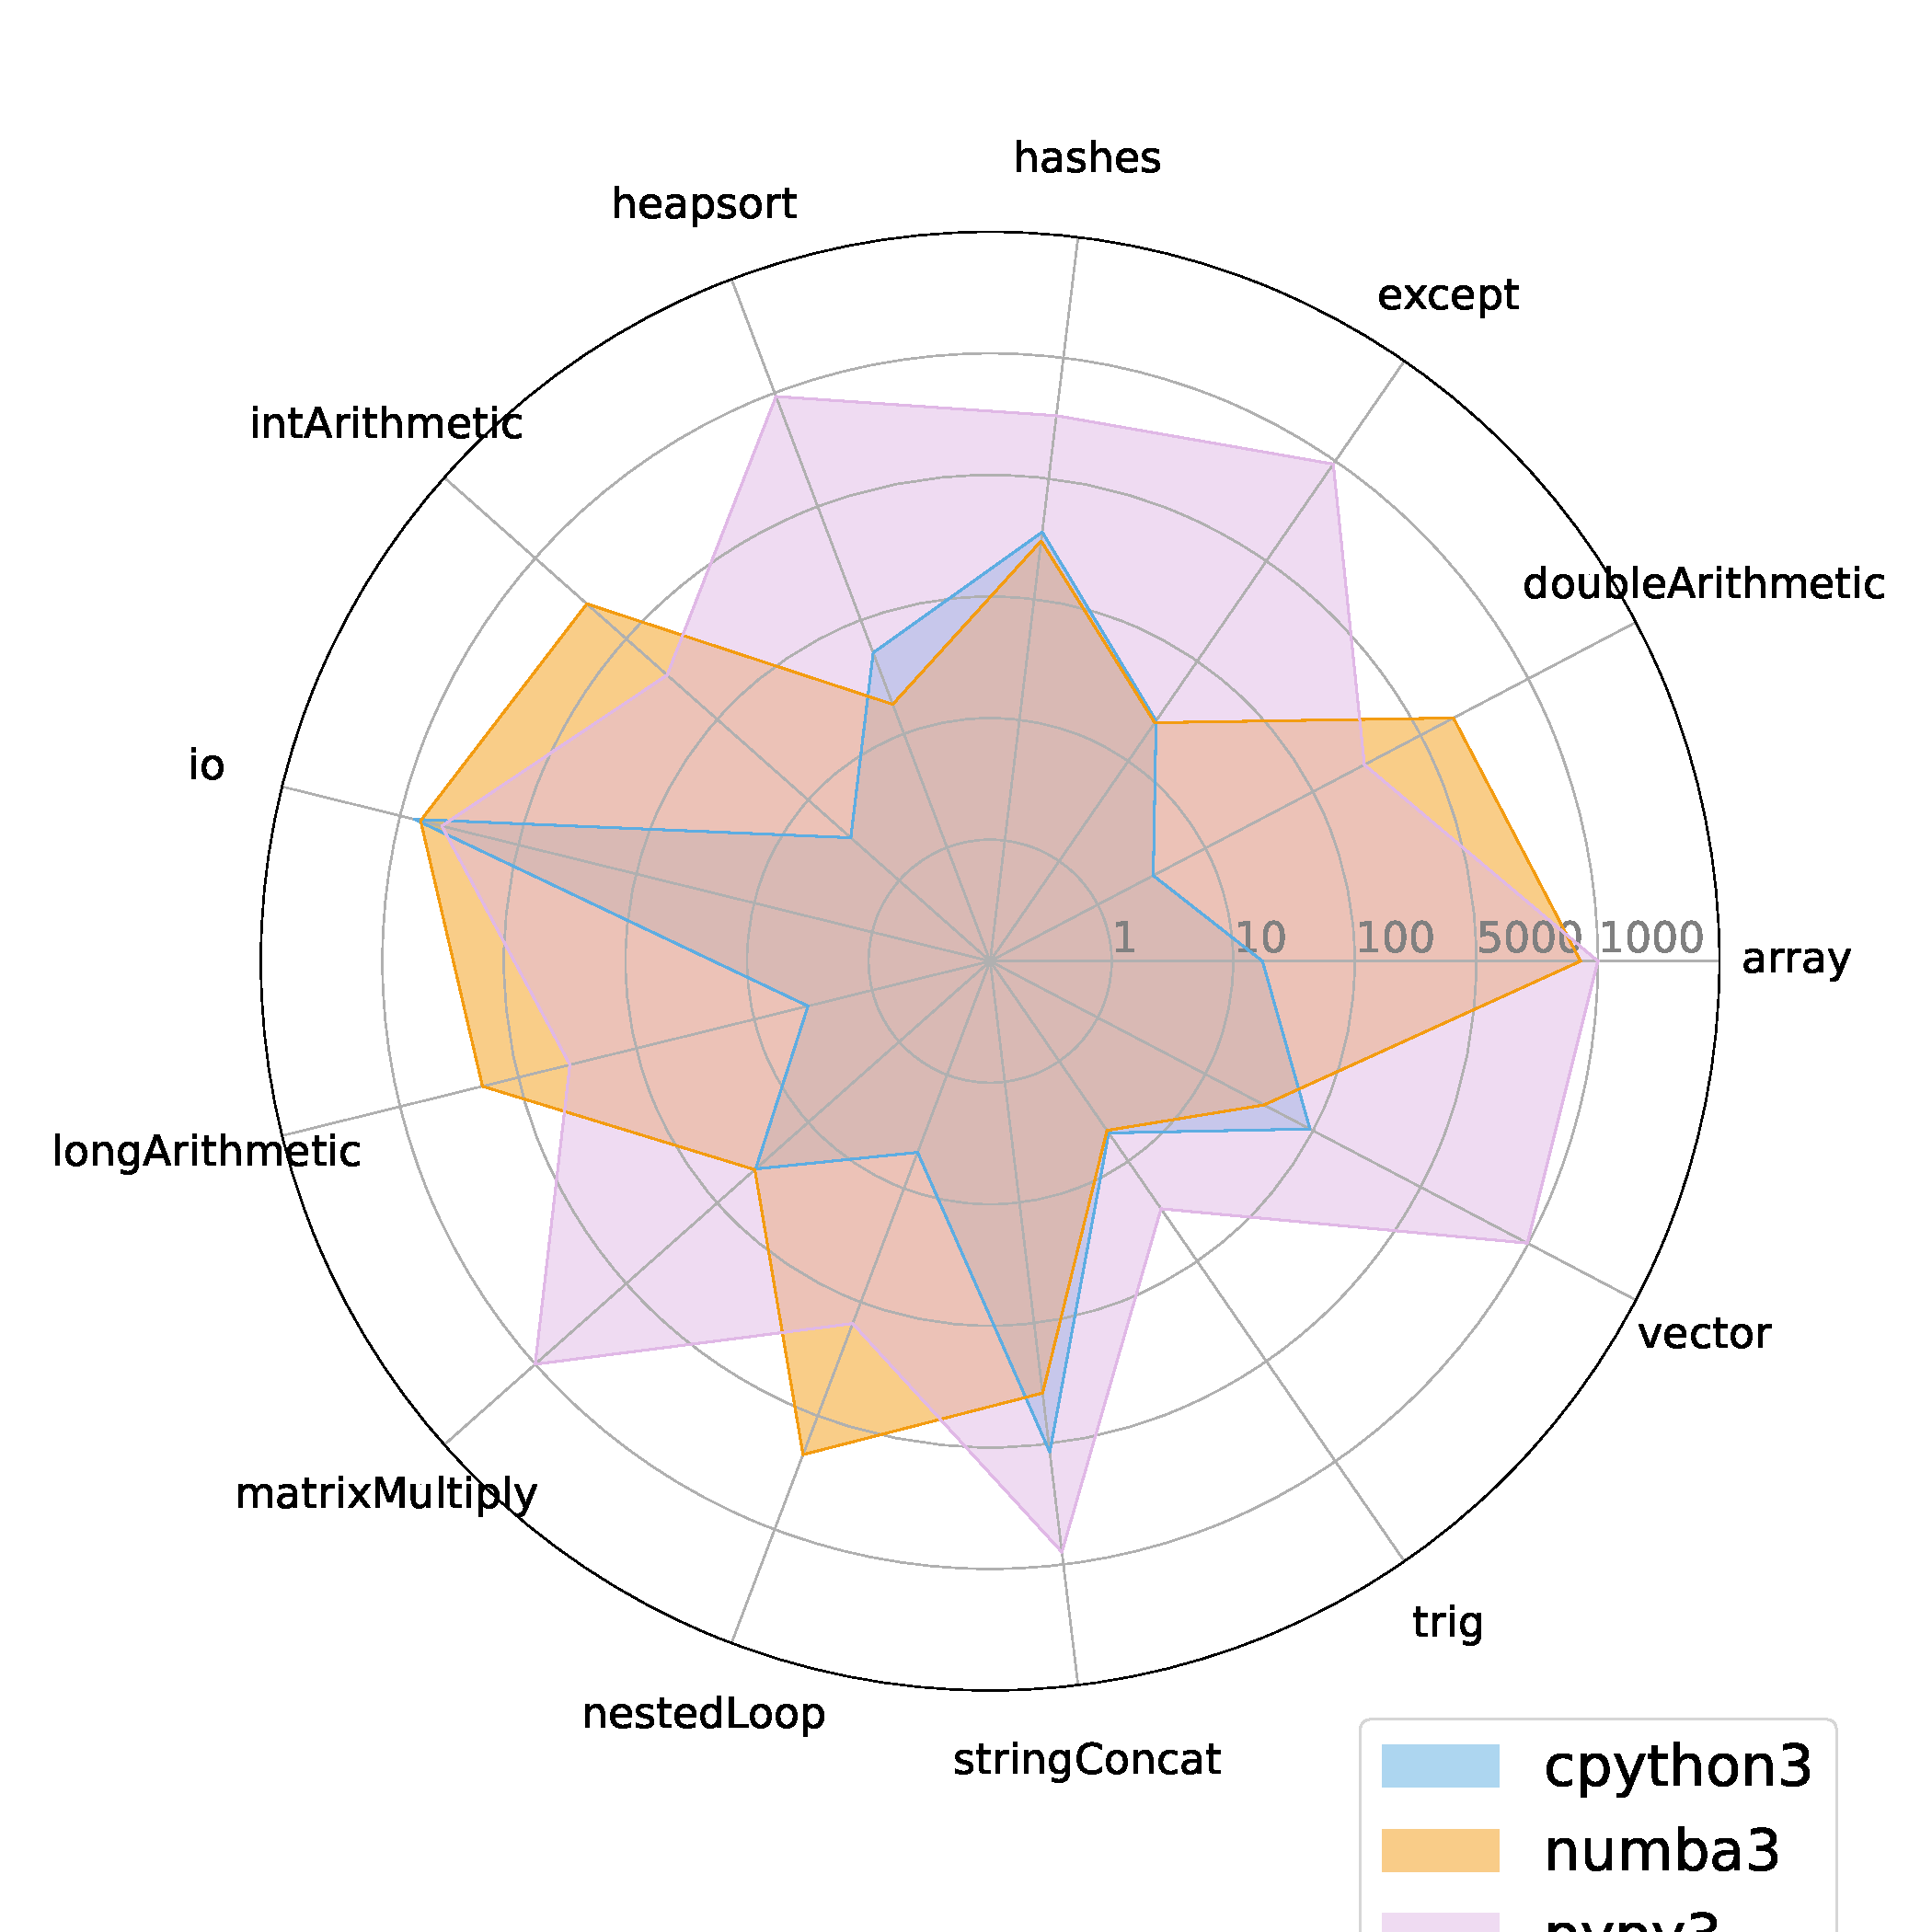
\includegraphics[width=\linewidth]{imgs/tommti_compare__cpython3_numba3_pypy3}
    \caption{comparaison of pypy vs python vs numba }
    \label{fig:p3}
\end{figure}

\begin{figure}
    \centering
    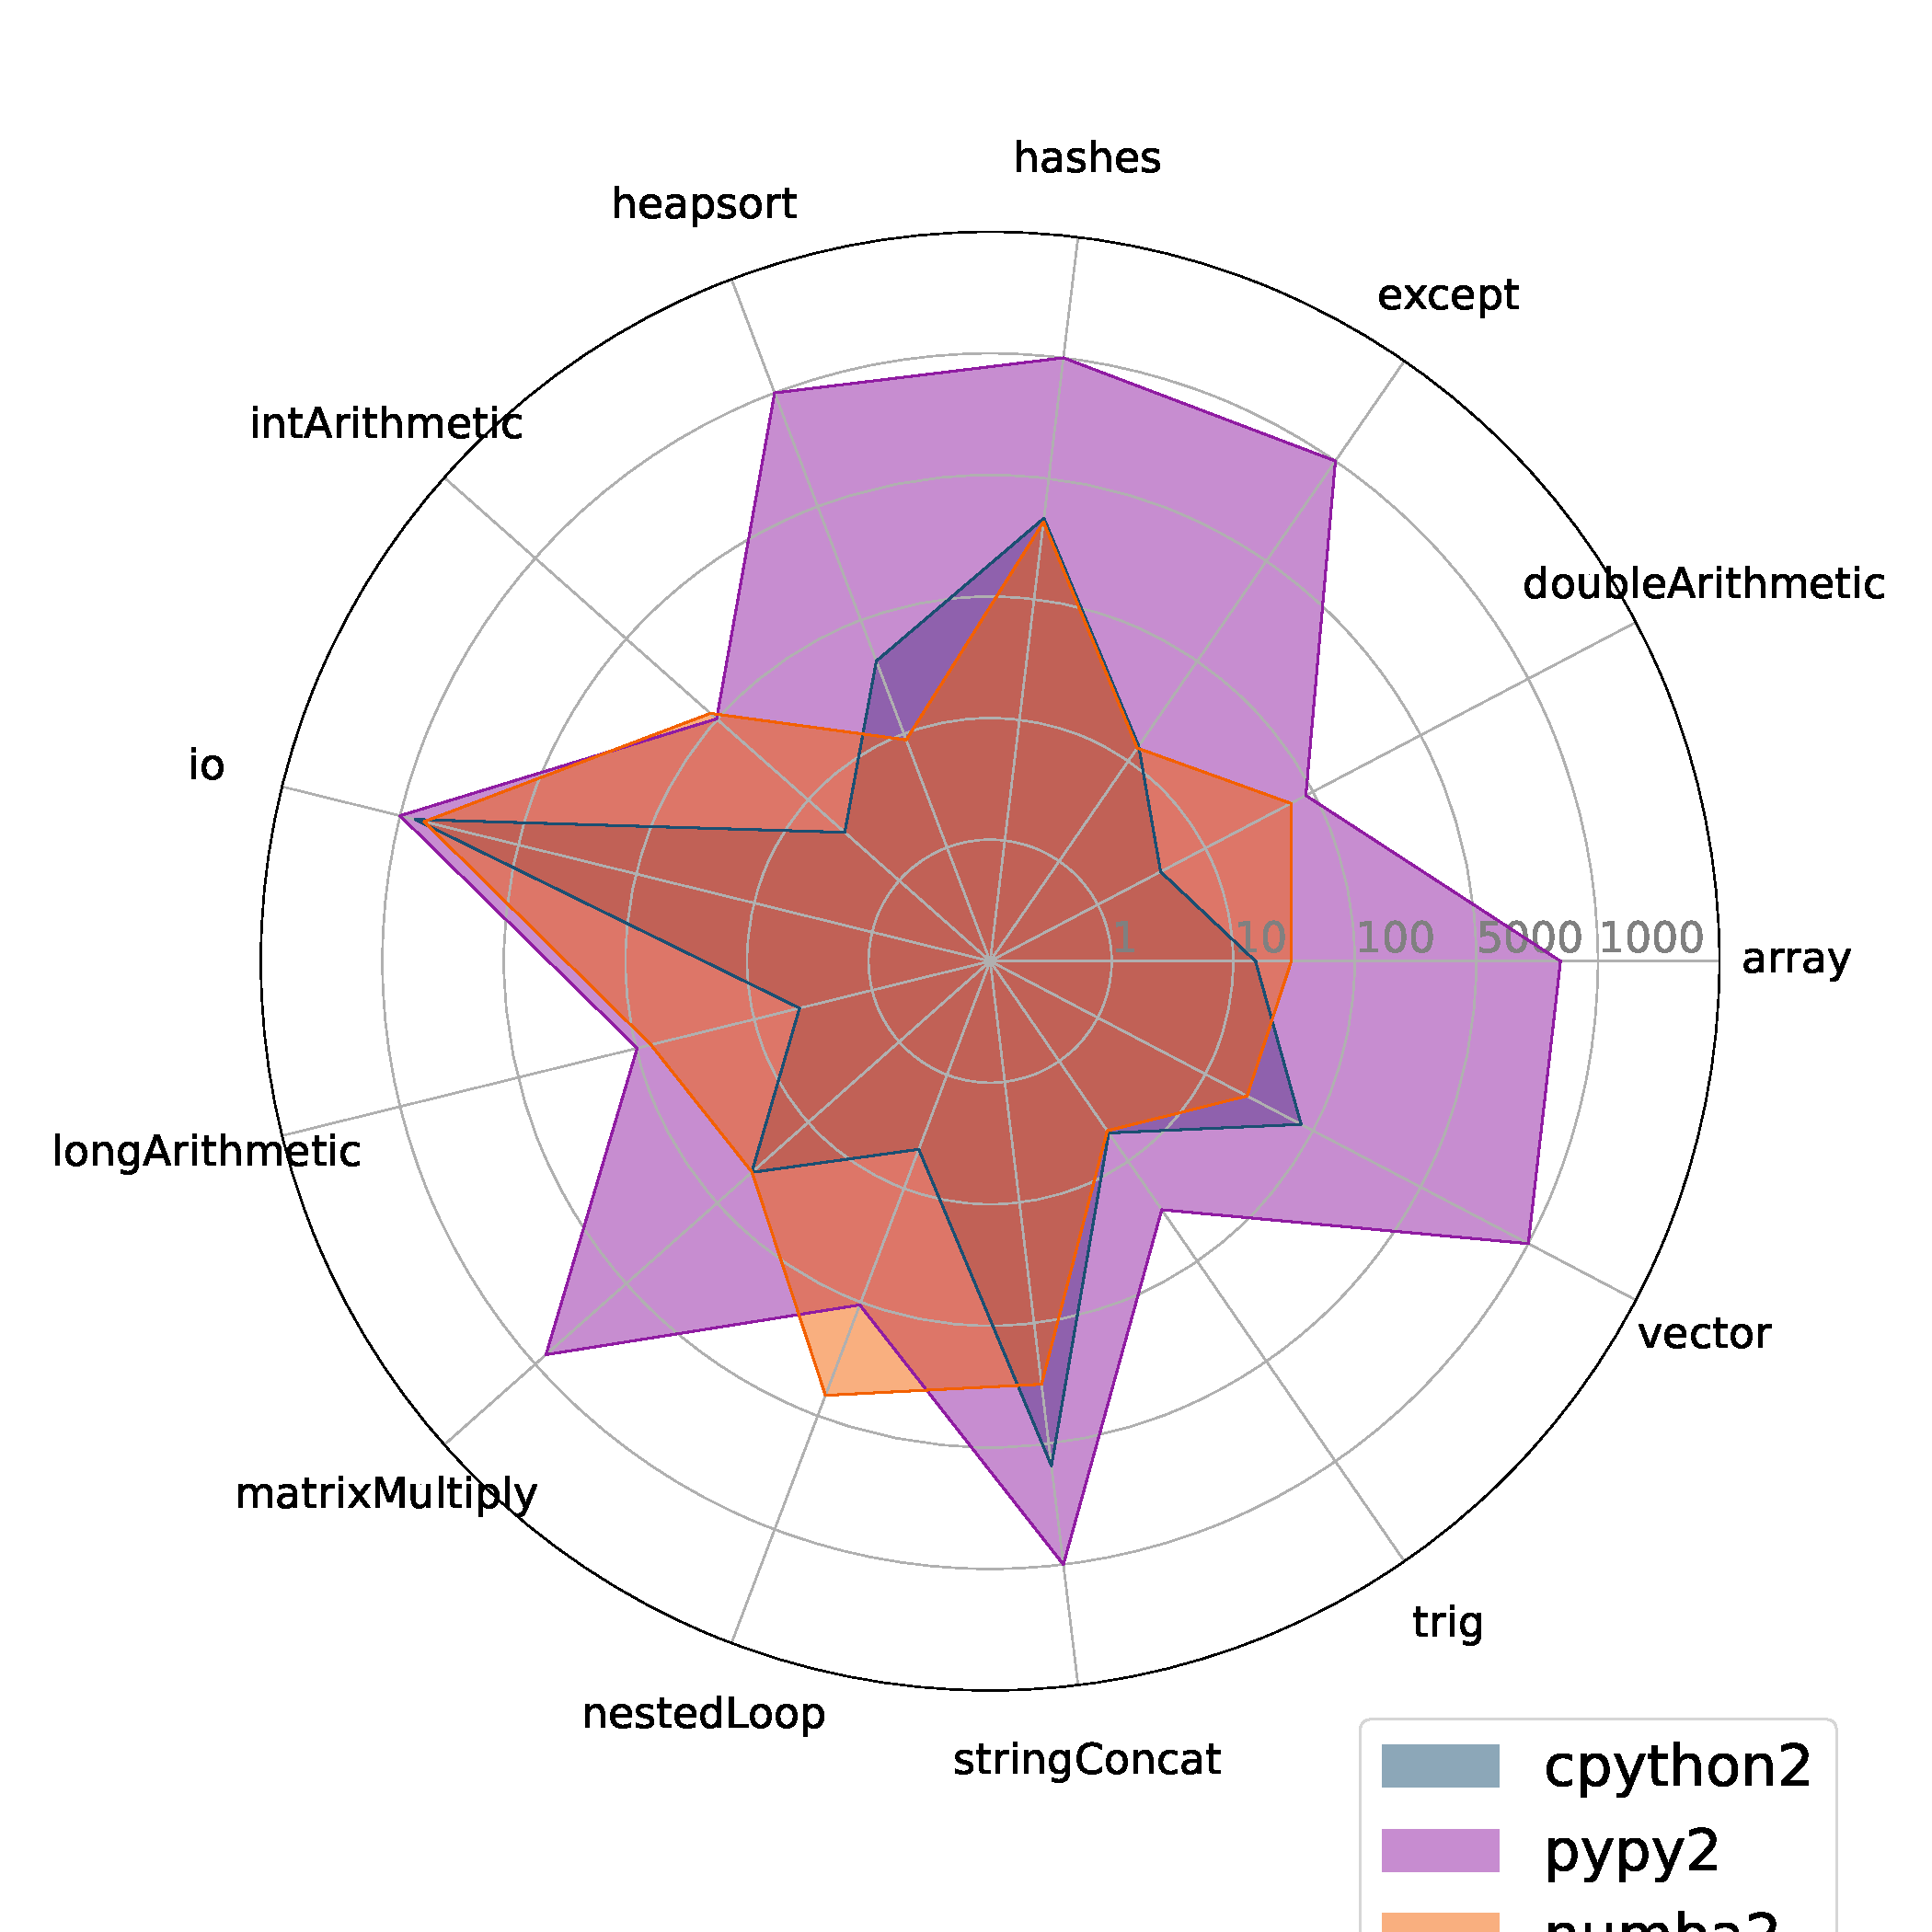
\includegraphics[width=\linewidth]{imgs/tommti_compare__cpython2_pypy2_numba2}
    \caption{comparaison of pypy vs python vs numba }
    \label{fig:p2}
\end{figure}

As we can see in figure \ref{fig:tommi_all}, there is no evolution between cpython2 and cpython3
Intelpython and active python both folows the same behaviour. one can conclude that the work that have been on those interpreters is mainly
to improve a specific purpose, Active python claims that their version is focused on secuirty which explains the lack of some performances due to the introduction of more reonforcment
.Morver Intel published their version of python as a dedicated for machine learning. Unfortunately the tommti benchmark is a set that focuses on the general purpose programming
which does not reflect the performance of the machine learning.
Another aspect of a such behaviour might be due to the fact of the processors that were used in the testbed. and it might change in the future if we include the GPU part for the machine learning benchmarks
% reference the work of the intern 
As for nuitka. there were no optimization in the energy consumpotion despite the fact that is it a complier.
However if we dig through the nuitka mechanisms. they basically embed the python code with an interpreter.
Unllike nuitka shedskin exhebit a the best energy consumption pattern when it comes to the arithmetic operartions. One can conclude it is due to the fact of the native type of the variables. unlike the interpreters where they are treated as object in the begining.

for the other interpeters pypy is very promising especially when it comes to data maniupulation as one can see in the figure \ref{fig:bar_tommti_vector}
pypy is by far the best interperer when it comes to treating vectors.
numba2 introduced the JIT but wasn't as promising as numba3.

for the other vm based interpereters. jython and ipy lacked in term of energy optimisation which was kinda expected since they were in their the begining of the stage and the main puprose of such implementation is to link the bytecode generated by jython and ironpython with their respectives virtual machin.

Unlike the the previous interpeters. graal exhebits a certin promises when it comes to complex algorithms - nested loops -
micro python is dedicated to embeded systems so lunching it is powerful cpu machines will be misleading.

Most of the interperters had the same behaviour when it comes to the input outputs. except for jython which was kinda of a anomaly probably due to the lack of the optimizations.
% pypy handles exceptions very well 


\section{conclusion}
One may observe that the choice of Python interpreter has a significant impact on the programs' energy consumption.
This investigation is made more intriguing by the absence of a universal solution.
The primary downside is the incompatibility of some of these solutions, which causes us to make concessions when we need a generic answer.



% \subsection{threads to validity \note{missing}}
\clearpage
\section{Conclusion}
As many software services use Python in public and private cloud infrastructures, making Python-based apps more energy efficient will lower ICT carbon emissions.
This chapter discusses various ways of optimizing the energy consumption of Python-based applications.
It first explains why such a choice is relevant.
Then, it studies the energy behavior of Python within its most commonly employed use cases, which are revealed to be web development and machine learning.

First, we studied the energy consumption of a machine learning algorithm using a benchmark of $60,000$ entries to train the \texttt{cifar10-fast} model.
We discovered that this energy consumption increases exponentially while the model accuracy increases.
As a result, a reduction in accuracy can result in considerable energy savings.
We investigated how data structures, parallelism, and iterative methods affect energy use.

As for web development, we study a website built with Django, which is one of the most popular web frameworks in the Python community.
We found that fetching the data from the database consumes most of the energy during the request processing phase.
Therefore, Django-based web servers can use up to ten times less energy if the developer chooses the write strategy to fetch the data.

After that, we analyzed the impact of several iteration mechanisms in Python and their impact on energy consumption.
We found that the built-in functions and the best practices for writing Python code are the most energy-efficient ones.
This energy efficiency is because most of these built-in functions are written in a lower programming language, C.

Finally, we studied the impact of concurrency on energy consumption for Python applications.
We found that the multi-processing strategy is the most energy-efficient one.
However, this strategy should be used cautiously.
This study demonstrates that the optimal number of processes is equal to the number of physical cores, and exceeding this number will cause the application to lose its efficiency in both performance and energy consumption.
As for the multithreading strategy, we found that the Python interpreter is not thread-safe, which leads to a slower performance than the sequential one.
However, this also leads to lower power consumption, which sometimes overcomes the lack of performance to make the application more energy-efficient.

In the second section, we presented a non-intrusive technique to optimize the energy consumption of Python-based apps without making substantial changes to the code.
This technique consists in guiding the choice of the Python runtime implementation.
We started by categorizing and filtering these implementations into three significant classes (compiler, interpreter, and extra libraries).
Then, we conducted a series of experiments to compare the energy consumption of these alternatives.
Our findings indicate the lack of a general solution and the importance of tuning the Python runtime depending on the application.
% In some circumstances, some of these answers may be the best, while others may be the worst.
We found that most interpreters had a similar or worse energy consumption than the official implementation of CPython.
The reason behind such behavior was that some implementations focused on specific case studies, such as machine learning or security.
In contrast, others focused on the compatibility of the Python code with their platforms, like Jython and IronPython.
Finally, regardless of implementation, we demonstrated that using JIT is the most efficient technique to boost the energy efficiency of Python-based programs.

We believe that our contributions will benefit a broad spectrum of legacy systems, reducing ICT's carbon footprint and lowering cloud bills for these services' resources.